\documentclass[a4paper,12pt]{article}
\usepackage{fontspec}
\usepackage{xeCJK}
\setmainfont{Times New Roman}
\usepackage{amsmath}
\usepackage{amsthm}
\usepackage{amsfonts}
\usepackage{amssymb}
\usepackage{graphicx}
\usepackage{hyperref}
\usepackage{enumitem}
\usepackage{textcomp}
\usepackage{float}
\usepackage{booktabs}
\usepackage[colorinlistoftodos]{todonotes}
\usepackage[left=1.50cm, right=1.50cm, top=1.20cm]{geometry}
\linespread{1.5}
\usepackage{algorithm}
\usepackage{algpseudocode}
\usepackage{tikz}
\usetikzlibrary{matrix, positioning, fit, arrows, calc, intersections, shapes, shadings, patterns, decorations.markings, chains, scopes, arrows.meta, shapes.geometric}
\usepackage{upquote}
\usepackage{listings}
\usepackage{color}
\usepackage{subcaption}
\usepackage[tikz]{mdframed}
\lstdefinestyle{customc}{
  belowcaptionskip=1\baselineskip,
  breaklines=true,
  frame=L,
  xleftmargin=\parindent,
  language=C++,
  tabsize=2,
  %numbers=left,
  %stepnumber=1,
  showstringspaces=false,
  basicstyle=\small\ttfamily,
  keywordstyle=\bfseries\color{green!40!black},
  commentstyle=\itshape\color{purple!40!black},
  identifierstyle=\color{blue},
  stringstyle=\color{orange},
}
\mdfdefinestyle{mymdf}{leftmargin=1cm,rightmargin=2cm,%
innerleftmargin=1cm,innerrightmargin=1cm,roundcorner=10pt,backgroundcolor=lg}
\definecolor{lg}{RGB}{247,249,250}
\title{Algorithm Problem Set \\ \large No. 200 --- 299}
\author{SS}
\date{Feburary 2019}

\begin{document}
\renewcommand{\thelstlisting}{\thesection.\arabic{lstlisting}}

\newcommand{\fcc}[1]{\lstinline[language=C++, basicstyle=\small\ttfamily, keywordstyle=\bfseries\color{green!40!black}]|#1|}
\newcommand{\fcj}[1]{\lstinline[language=Java, basicstyle=\small\ttfamily, keywordstyle=\bfseries\color{green!40!black}]|#1|}
%\sloppy
\maketitle
%\section{201 --- Bitwise AND of Numbers Range}
Given a range $[m, n]$ where $0 \leq m \leq n \leq 2147483647$, return the bitwise \textbf{AND} of all numbers in this range, inclusive.
\paragraph{Example 1:}
\begin{flushleft}
\textbf{Input}: $[5,7]$
\\
\textbf{Output}: 4
\end{flushleft}
\paragraph{Example 2:}
\begin{flushleft}
\textbf{Input}: $[0,1]$
\\
\textbf{Output}: 0
\end{flushleft}
\subsection{Find Common Left Part}
先从题目中给的例子来分析,$[5, 7]$里共有三个数字,其二进制分别为:
$101\;110\;111$

Bitwise AND后的结果为100,仔细观察可以看出,最后的数是该数字范围内所有的数的左边共同的部分。

再以$[26, 30]$为例,它们的二进制如下:

$11010\;11011\;11100\;11101\;11110$

Bitwise AND后的结果为11000。

因此程序所作的就是找到找到范围内所有数左边公共的部分。算法步骤包括
\begin{itemize}
\item 建立一个32位都是1的mask,
\item 每次把mask左移一位。然后看$m$与mask做bitwise AND后的结果与$n$ Bitwise AND mask后的结果是否相同。
\item 最后$m$和mask bitwise AND 的结果就是最终结果
\end{itemize}

\setcounter{lstlisting}{0}
\begin{lstlisting}[style=customc, caption={Find Common Left Bits}]
int rangeBitwiseAnd( int m, int n )
{
    int mask = INT_MAX;
    int zero_mask = 1;
    while( m != n )
    {
        mask ^= zero_mask; //left shift mask to add zero at its right
        zero_mask <<= 1;
        m &= mask;
        n &= mask;
    }
    return m;
}
\end{lstlisting}
\subsection{Removing rightest bit 1}
The key point: reduce $n$ by removing the rightest 1 bit until $n\leq m$;
\begin{lstlisting}[style=customc, caption={Remove rightest bit 1}]
int rangeBitwiseAnd( int m, int n )
{
    while( m < n )
    {
        n = ( n & ( n - 1 ) ); // remove rightest bit 1 from n
    }
    return n;
}
\end{lstlisting}
%\section{202 --- Happy Number}
Write an algorithm to determine if a number is \textit{happy}.
\par
A happy number is a number defined by the following process: 
\par
Starting with any positive integer, replace the number by the sum of the squares of its digits, and repeat the process until the number equals 1 (where it will stay), or it loops endlessly in a cycle which does not include 1. Those numbers for which this process ends in 1 are \textit{happy numbers}.
\paragraph{Example: }
\begin{flushleft}

\textbf{Input}: 19
\\
\textbf{Output}: \texttt{true}
\\
\textbf{Explanation}: 
\begin{align*}
1^2 + 9^2 &= 82\\
8^2 + 2^2 &= 68\\
6^2 + 8^2 &= 100\\
1^2 + 0^2 + 0^2 &= 1\\
\end{align*}
\end{flushleft}
\subsection{Hash Set}
\begin{CJK*}{UTF8}{gbsn}
可以用hash set来记录所有出现过的数字,然后每出现一个新数字,在set中查找看是否存在
\end{CJK*}
\setcounter{lstlisting}{0}
\begin{lstlisting}[style=customc, caption={Hash Set}]
bool isHappy( int n )
{
    unordered_set<int> s;
    s.insert( n );

    while( true )
    {
        int m = n;
        int sum = 0;

        while( m )
        {
            int q = m / 10;
            int r = m - 10 * q;

            sum += ( r * r );
            m = q;
        }

        if( sum == 1 )
        {
            return true;
        }

        if( s.find( sum ) != s.end() )
        {
            return false;
        }

        s.insert( sum );

        n = sum;
    }

    return false;
}

\end{lstlisting}
\subsection{Mathematical Induction}
\begin{CJK*}{UTF8}{gbsn}
Non happy number有个特点,循环的数字中必定会有4
\end{CJK*}
\begin{lstlisting}[style=customc, caption={Mathematical Induction}]
bool isHappy( int n )
{
    while( n != 1 && n != 4 )
    {
        int t = 0;
        while( n )
        {
            t += ( n % 10 ) * ( n % 10 );
            n /= 10;
        }
        n = t;
    }
    return n == 1;
}
\end{lstlisting}
%\section{203 --- Remove Linked List Elements}
Remove all elements from a linked list of integers that have value $v$.
\paragraph{Example}:
\begin{flushleft}
\textbf{Input}:

\begin{figure}[H]
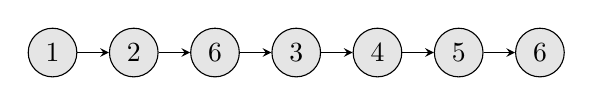
\begin{tikzpicture}
[mynode/.style={draw,circle,minimum size=5mm, fill=gray!20!}]
\node(){};
\node[mynode](1) {1};
\node[mynode](2)[right=4mm of 1] {2};
\node[mynode](3)[right=4mm of 2] {6};
\node[mynode](4)[right=4mm of 3] {3};
\node[mynode](5)[right=4mm of 4] {4};
\node[mynode](6)[right=4mm of 5] {5};
\node[mynode](7)[right=4mm of 6] {6};
\draw[>=stealth,->] (1) -- (2);
\draw[>=stealth,->] (2) -- (3);
\draw[>=stealth,->] (3) -- (4);
\draw[>=stealth,->] (4) -- (5);
\draw[>=stealth,->] (5) -- (6);
\draw[>=stealth,->] (6) -- (7);
\end{tikzpicture}
\end{figure}
$v=6$
\\
\textbf{Output}:
\begin{figure}[H]
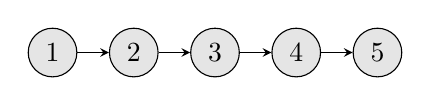
\begin{tikzpicture}
[mynode/.style={draw,circle,minimum size=5mm, fill=gray!20!}]
\node(){};
\node[mynode](1) {1};
\node[mynode](2)[right=4mm of 1] {2};
\node[mynode](3)[right=4mm of 2] {3};
\node[mynode](4)[right=4mm of 3] {4};
\node[mynode](5)[right=4mm of 4] {5};
\draw[>=stealth,->] (1) -- (2);
\draw[>=stealth,->] (2) -- (3);
\draw[>=stealth,->] (3) -- (4);
\draw[>=stealth,->] (4) -- (5);
\end{tikzpicture}
\end{figure}
\end{flushleft}
\subsection{Dummy Header}
创建一个dummy header,用它的\texttt{next}指向\texttt{head},这样就能很好避免很多判断了。
\setcounter{lstlisting}{0}
\begin{lstlisting}[style=customc, caption={Dummy Header}]
ListNode* removeElements( ListNode* head, int val )
{
    ListNode *dummy = new ListNode( -1 );
    dummy->next = head;
    auto cur = head;
    auto pre = dummy;
    while( cur )
    {
        if( cur->val == val )
        {
            auto next = cur->next;
            cur->next = nullptr;
            pre->next = next;
            cur = next;
        }
        else
        {
            pre = cur;
            cur = cur->next;
        }
    }

    return dummy->next;
}

\end{lstlisting}
%\section{204 --- Count Primes}
Count the number of prime numbers less than a non-negative number, $n$.
\paragraph{Example:}

\begin{flushleft}
\textbf{Input}: 10
\\
\textbf{Output}: 4
\\
\textbf{Explanation}: 
\\
There are 4 prime numbers less than 10, they are 2, 3, 5, 7.
\end{flushleft}
\subsection{Sieve of Eratosthenes}
\begin{itemize}
\item 从2开始遍历到$\sqrt{n}$,
\item 先找到第一个质数2,然后将其所有的倍数全部标记出来,
\item 然后到下一个质数3,标记其所有倍数,
\item 依次类推,直到$\sqrt{n}$,此时数组中未被标记的数字就是质数。
\end{itemize}
maintain 一个 $n-1$ 长度的数组来记录每个数字是否被标记,长度为$n-1$的原因是题目说是小于$n$的质数个数,并不包括$n$。

\setcounter{lstlisting}{0}
\begin{lstlisting}[style=customc, caption={Sieve of Eratosthenes}]
int countPrimes( int n )
{
    if( n <= 2 )
    {
        return 0;
    }
    vector<unsigned char> A( n - 1, 1 );

    A[0] = 0; // 1 is not a prime number

    int i = 2;

    while( i * i <= n )
    {
        if( A[i - 1] == 1 )
        {
            for( int j = i * i; j < n; j += i )
            {
                A[j - 1] = 0;
            }
        }

        ++i;
    }

    int ans = accumulate( A.begin(), A.end(), 0 );

    return ans;
}
\end{lstlisting}
%\section{205 --- Isomorphic Strings}
Given two strings $s$ and $t$, determine if they are isomorphic.
\par
Two strings are \textit{isomorphic} if the characters in $s$ can be replaced to get $t$.
\par
All occurrences of a character must be replaced with another character while preserving the order of characters. No two characters may map to the same character but a character may map to itself.
\paragraph{Example 1:}
\begin{flushleft}
\textbf{Input}: $s = \texttt{egg}$, $t = \texttt{add}$
\\
\textbf{Output}: \texttt{true}
\end{flushleft}

\paragraph{Example 2:}
\begin{flushleft}
\textbf{Input}: $s = \texttt{foo}$, $t = \texttt{bar}$
\\
\textbf{Output}: \texttt{false}
\end{flushleft}

\paragraph{Example 3:}
\begin{flushleft}
\textbf{Input}: $s = \texttt{paper}$, $t = \texttt{title}$
\\
\textbf{Output}: \texttt{true}
\end{flushleft}
\paragraph{Note:}
\begin{itemize}
    \item You may assume both s and t have the same length.
\end{itemize}
\subsection{Hash Map}
\begin{CJK*}{UTF8}{gbsn}
用两个哈希表分别来记录原字符串和目标字符串中字符出现情况,由于ASCII码只有256个字符,所以可以用一个256大小的数组来代替哈希表,并初始化为0,
\par
然后遍历原字符串,在当前index $i$。分别在两个哈希表中查找$s[i]$和$t[i]$对应的值,若不相等,则返回\texttt{false},若相等,将两个hash map中对应的值更新为$i + 1$
\end{CJK*}
\setcounter{algorithm}{0}
\begin{algorithm}[H]
\caption{Two Hash Map}
\begin{algorithmic}[1]
\Procedure{isIsomorphic}{$S, T, L$}
\State $\star$ Create two arrays $x$ and $y$. Each array has 256 elements that initialized to zero
\For{$i:=0 \to L-1$}
\If{$x[s[i]]\neq y[t[i]]$}
\State \Return \texttt{false}
\EndIf
\State $\star$ Use $i+1$ to avoid zero as the value
\State $x[s[i]]\gets i+1$ 
\State $y[s[i]]\gets i+1$
\EndFor
\State \Return \texttt{true}
\EndProcedure
\end{algorithmic}
\end{algorithm}
\setcounter{lstlisting}{0}
\begin{lstlisting}[style=customc, caption={Two Hash Maps}]
  bool isIsomorphic(string s, string t) {

        vector<int> x(256, 0);

        vector<int> y(256, 0);
        
        for(size_t i = 0; i < s.size(); ++i)
        {
            if(x[s[i]] != y[t[i]])
            {
                return false;
            }
            
            x[s[i]] = i+1;
            y[t[i]] = i+1;
        }

        return true;
        
    }
\end{lstlisting}
%\section{206 --- Reverse Linked List}
A linked list can be reversed either iteratively or recursively. Could you implement both?
\subsection{Iterative}
Starting from the beginning, for each node
\begin{itemize}
    \item Save its \texttt{next} to a temporary variable $\alpha$
    \item Change its \texttt{next} to previous node
    \item Move to $\alpha$
\end{itemize}
\setcounter{lstlisting}{0}
\begin{lstlisting}[style=customc, caption={Iterative}]
ListNode* reverseList(ListNode* head)
{

    ListNode* pre = nullptr;
    
    auto cur = head;
    
    while(cur)
    {
        auto next = cur->next;
        cur->next = pre;
        pre = cur;
        cur = next;
    }
    
    return pre;

}
\end{lstlisting}
\subsection{Recursion}
The recursive version is slightly trickier and the key is to work backwards. Assume that the rest of the list had already been reversed, now how to reverse the front part?
\par
Assumes the list is 
\par
$n_1\to\ldots\to n_{k-1}\to n_k\to n_{k+1}\to\ldots\to n_m\to \varnothing$
\par
Assume from node $n_{k+1}$ to $n_m$ has been reversed and now at node $n_{k}$, as shown below
\par
$n_1\to\ldots\to n_{k-1}\to \mathbf{n_k}\to n_{k+1}\longleftarrow\ldots\longleftarrow n_m$
\par
What need to do is change $n_{k+1}$'s \texttt{next} to point to $n_k$, therefore
\par
$n_k.\texttt{next}.\texttt{next}\gets n_k$
\par
An important note is that $n_1$'s \texttt{next} must point to $\varnothing$. Otherwise, the linked list has a cycle in it.
\begin{lstlisting}[style=customc, caption={Recursion}]
ListNode* reverseList(ListNode* head)
{
    if(!head ||(!head->next))
    {
        return head;
    }
    
    auto p = reverseList(head->next);
    
    head->next->next = head;
    
    head->next = nullptr;
    
    return p;
}
\end{lstlisting}
\section{207 --- Course Schedule}
There are a total of $n$ courses you have to take, labeled from 0 to $n-1$.
\par
Some courses may have prerequisites, for example to take course 0 you have to first take course 1, which is expressed as a pair: $[0,1]$
\par
Given the total number of courses $n$ and a list of prerequisite pairs $P$, is it possible for you to finish all courses?
\paragraph{Example 1:}
\begin{flushleft}
\textbf{Input}: $2$, $[[1,0]]$
\\
\textbf{Output}: \texttt{true}
\\
\textbf{Explanation}:
\\
There are a total of 2 courses to take. To take course 1 you should have finished course 0. So it is possible.
\end{flushleft}
\paragraph{Example 2:}
\begin{flushleft}
\textbf{Input}: $2$, $[[1,0],[0,1]]$
\\
\textbf{Output}: \texttt{false}
\\
\textbf{Explanation}:
\\
There are a total of 2 courses to take. To take course 1 you should have finished course 0, and to take course 0 you should also have finished course 1. So it is impossible.
\end{flushleft}
\paragraph{Note:}
\begin{itemize}
    \item The input prerequisites is a graph represented by a list of edges, not adjacency matrices. Read more about how a graph is represented.
    \item You may assume that there are no duplicate edges in the input prerequisites.
\end{itemize}
\subsection{DFS}
To detect cycle in directed graph, mark the visited node as one color number like 1. And then if there is a cycle, some nodes that has already been colored as $1$ could be meeted again. If there is no cycle, Otherwise, after the DFS is done for this starting node, mark this node as another color number like 2.
\setcounter{algorithm}{0}
\begin{algorithm}[H]
\caption{DFS}
\begin{algorithmic}[1]
\State $\star$ $P$ is the prerequisite pair array with length $L$ and $L$ may not equal to $n$
\Procedure{CanFinish}{$n, P, L$}
\State $\star$ Build a adjacent graph structure $G$ from $P$
\State $\star$ Create a array $x$ which records each node's marked color, initially, all nodes are colored as 0
\For{$\alpha \in G$} \Comment Iterate through each outgoing node in $G$
\State $b:=$ \Call{DFS}{$\alpha, G, x$}
\If{$b=\texttt{false}$}
\State \Return $b$ \Comment Found cycle in $G$
\EndIf
\State \Return \texttt{true}
\EndFor
\EndProcedure
\end{algorithmic}
\end{algorithm}
Function \texttt{DFS} color each node by number 2. Before the depth first search process, the starting node is marked by number 1. If a node marked by number 1 meet again, there is a cycle in the graph. 
\begin{algorithm}[H]
\caption{Helper Function}
\begin{algorithmic}[1]
\Function{DFS}{$\alpha, G, x$}
\If{$x[\alpha]=2$} \Comment This node has been visited
\State \Return \texttt{true}
\EndIf
\If{$x[\alpha]=1$} \Comment This node is found by back edge so there is a cycle
\State \Return \texttt{false}
\EndIf
\State $x[\alpha]\gets 1$ \Comment Color the node as 1 indicate DFS is going on from this node
\For{$t \in G[\alpha]$} \Comment Iterate through each connected node of $\alpha$
\State $b:=$ \Call{DFS}{$t, G, x$}
\If{$b = \texttt{false}$} \Comment There is a cycle
\State \Return \texttt{false}
\EndIf
\algstore{207algo}
\end{algorithmic}
\end{algorithm}
\begin{algorithm}[H]
\begin{algorithmic}[1]
\algrestore{207algo}
\EndFor
\State $x[\alpha]\gets 2$ \Comment Color the node as 2 indicate this node has survived the DFS process
\EndFunction
\end{algorithmic}
\end{algorithm}
\setcounter{lstlisting}{0}
\begin{lstlisting}[style=customc]
bool canFinish( int numCourses, vector<pair<int, int>>& prerequisites )
{
    unordered_map<int, unordered_set<int>> g;

    for( const auto& p : prerequisites )
    {
        auto it = g.find( p.second );

        if( it == g.end() )
        {
            g.emplace( p.second, initializer_list<int> {p.first} );
        }
        else
        {
            it->second.insert( p.first );
        }
    }

    vector<int> color( numCourses, 0 );

    for( const auto& p : g )
    {
        int start = p.first;
        if( !dfs( g, start, color ) )
        {
            return false;
        }
    }

    return true;
}

bool dfs( unordered_map<int, unordered_set<int>>& g, int x, vector<int>& color )
{
    if( color[x] == 2 )
    {
        //visited before
        return true;
    }

    if( color[x] == 1 )
    {
        //visited but still in DFS process
        return false;
    }

    //Mark color of x as 1 which means DFS is started and in the progress
    color[x] = 1;

    for( int y : g[x] )
    {
        if( !dfs( g, y, color ) )
        {
            return false;
        }
    }

    color[x] = 2; //Mark color of x as 2. Survivied DFS search

    return true;
}
\end{lstlisting}
\subsection{BFS}
The idea is to simply use \textbf{Topological Sorting}
\begin{enumerate}
    \item Get in-degree (number of incoming edges) for each of the vertex present in the graph and initialize the count of visited nodes as 0.
    \item Pick all the vertices with in-degree as 0 and add them into a queue $Q$
    \item Pop a vertex from $Q$ and then
    \begin{itemize}
        \item increment count of visited nodes by 1. 
        \item Decrease in-degree by 1 for all its neighboring nodes.
    \item If in-degree of a neighboring nodes is reduced to zero, then add it to $Q$.
\end{itemize}
\item Repeat 3 until $Q$ is empty.
\item If count of visited nodes is not equal to the number of nodes in the graph, then there exits a cycle.
\end{enumerate}
\begin{algorithm}[H]
\caption{BFS}
\begin{algorithmic}[1]
\Procedure{CanFinish}{$n, P, L$}
\State $\star$ Build a adjacent graph structure $G$ from $P$
\State $\star$ Process array $P$ and put all nodes' in degree into an array $I$
\State $\star$ Initialize an empty queue $Q$
\For{$i:=0\to n-1$}
\If{$I[i]=0$} \Comment In-degree of node $i$ is zero
\State $Q\gets Q + (i)$ \Comment Push $i$ into the queue
\EndIf
\EndFor
\State $\delta:=0$ \Comment The number of visited nodes
\While{$Q\neq\emptyset$}
\State $\star$ Get the front of $Q$: $x$
\State $\star$ Pop front of $Q$
\State $\delta\gets\delta+1$ \Comment Increments the number of visited nodes
\algstore{207algo}
\end{algorithmic}
\end{algorithm}
\begin{algorithm}[H]
\begin{algorithmic}[1]
\algrestore{207algo}
\If{$G[x]\neq \emptyset$} \Comment $x$ has connected nodes
\For{$y \in G[x]$} \Comment Iterate all connected nodes of $x$
\If{$I[y] > 0$}
\State $I[y]\gets I[y]-1$ \Comment Decrements the in-degree of $y$
\If{$I[y] = 0$}
\State $\star$ Push $y$ into $Q$
\EndIf
\EndIf
\EndFor
\EndIf
\EndWhile
\If{$\delta\neq n$} \Comment Number of visited nodes does not equal to number of nodes
\State \Return \texttt{false} \Comment There exits a cycle
\Else
\State \Return \texttt{true}
\EndIf
\EndProcedure
\end{algorithmic}
\end{algorithm}
\setcounter{lstlisting}{0}
\begin{lstlisting}[style=customc, caption={BFS}]
bool canFinish( int numCourses, vector<pair<int, int>>& prerequisites )
{

    vector<int> idg( numCourses, 0 );

    unordered_map<int, unordered_set<int>> g;

    for( const auto& p : prerequisites )
    {
        ++idg[p.first];

        auto it = g.find( p.second );
        if( it == g.end() )
        {
            g.emplace( p.second, initializer_list<int> {p.first} );
        }
        else
        {
            it->second.insert( p.first );
        }
    }

    queue<int> q;

    int num_visited = 0;

    for( int i = 0; i < numCourses; ++i )
    {
        if( idg[i] == 0 )
        {
            q.push( i );
        }
    }

    while( !q.empty() )
    {
        int node = q.front();
        q.pop();

        ++num_visited;

        auto it = g.find( node );

        if( it == g.end() )
        {
            //node does not have any node connected
            continue;
        }

        for( int t : it->second )
        {
            if( idg[t] > 0 )
            {
                --idg[t]; //Decrease the in-degreee of t

                if( idg[t] == 0 )
                {
                    q.push( t );
                }
            }
        }
    }

    return num_visited == numCourses;

}
\end{lstlisting}
%\section{208 --- Implement Trie (Prefix Tree)}
Implement a \textbf{trie} with \texttt{insert}, \texttt{search}, and \texttt{startsWith} methods.
\paragraph{Example:}
\setcounter{lstlisting}{0}
\begin{lstlisting}[style=customc, caption={Example}]
Trie trie = new Trie();

trie.insert("apple");
trie.search("apple");   // returns true
trie.search("app");     // returns false
trie.startsWith("app"); // returns true
trie.insert("app");   
trie.search("app");     // returns true
\end{lstlisting}
\paragraph{Note:}
\begin{itemize}
\item You may assume that all inputs are consist of lowercase letters a--z.
\item All inputs are guaranteed to be non-empty strings.
\end{itemize}
\subsection{Array Of Pointers}
几个要点
\begin{itemize}
\item 需要一个root,不包含任何字符
\item 每个node需要一个标志位,表示是否代表一个单词。
\end{itemize}
\setcounter{lstlisting}{0}
\begin{lstlisting}[style=customc, caption={Trie Class}]
class Trie
{
public:
    /** Initialize your data structure here. */
    Trie()
    {
        m_root = new node();
    }

    /** Inserts a word into the trie. */
    void insert( string word )
    {
        auto p = m_root;

        for( auto c : word )
        {
            int i = c - 'a';
            if( !p->m_children[i] )
            {
                p->m_children[i] = new node();
            }
            p = p->m_children[i];
        }

		// This is a word
        p->m_isWord = true;
    }

    /** Returns if the word is in the trie. */
    bool search( string word )
    {
        auto p = m_root;

        for( auto c : word )
        {
            if( !p->m_children[c - 'a'] )
            {
                return false;
            }

            p = p->m_children[c - 'a'];

        }

        return p->m_isWord;
    }

    /** Returns if there is any word in the trie that starts with the given prefix. */
    bool startsWith( string prefix )
    {
        auto p = m_root;

        for( auto c : prefix )
        {
            if( !p->m_children[c - 'a'] )
            {
                return false;
            }

            p = p->m_children[c - 'a'];


        }

        return true;
    }

    struct node
    {
        vector<node*> m_children;
        bool m_isWord;

        node()
            : m_children( 26, nullptr )
            , m_isWord( false )
        {}
    };

	// Need a root as the start node
    node* m_root;
};


\end{lstlisting}
%\section{209 --- Minimum Size Subarray Sum}
Given an array of $n$ positive integers and a positive integer $s$, find the minimal length of a contiguous subarray of which the sum $\geq s$. If there isn't one, return 0 instead.
\paragraph{Example:}
\begin{flushleft}
\textbf{Input}: $s = 7$, $A = [2,3,1,2,4,3]$
\\
\textbf{Output}: 2
\\
\textbf{Explanation}: the subarray $[4,3]$ has the minimal length under the problem constraint.
\end{flushleft}
\paragraph{Follow up:}
\begin{itemize}
\item If you have figured out the $O(n)$ solution, try coding another solution of which the time complexity is $O(n \log n)$.
\end{itemize} 

\subsection{Sliding Window}
\begin{itemize}
\item 用$l$和$r$代表sliding window的左边界和右边界
\item 如果sliding window内的数字和小于$s$,则一直向右移动$r$,即扩大sliding window的宽度
\item 否则不停的向右移动$l$,即缩小这个sliding window。同时从$s$中去除缩小过程中不再包含在window中的数直至window内的数字和小于$s$。
\item 在3中,更新当前的window的宽度以及对应的全局最小宽度
\end{itemize}
\setcounter{lstlisting}{0}
\begin{lstlisting}[style=customc, caption={Sliding Window}]
int minSubArrayLen( int s, vector<int>& nums )
{
    int left = 0;
    int L = static_cast<int>( nums.size() );

    int right = 0;

    int sum = 0;

    int w = INT_MAX;

    while( right < L )
    {
        sum += nums[right];

        while( ( sum >= s ) && ( left <= right ) )
        {
            w = ( min )( w, right - left + 1 );
            sum -= nums[left];
            ++left;
        }

        ++right;
    }

    if( w == INT_MAX )
    {
        return 0;
    }

    return w;
}
\end{lstlisting}

\subsection{Binary Search}
\begin{itemize}
\item 用一个tree map存放从0到$i$的sum及其对应的$i$
\item 当$\sum\limits_{k=0}^iA[k] \geq s$时,计算两者之差$d$,然后在tree map中寻找第一个大于这个$d$的key,然后得到这个key的上一个key对应的$j$
\item 因为$\sum\limits_{k=j+1}^iA[k] \geq s$,所以与最小宽度比较进行更新。
\end{itemize}
\begin{lstlisting}[style=customc, caption={Binary Search}]
int minSubArrayLen( int s, vector<int>& nums )
{
    if( nums.empty() )
    {
        return 0;
    }

    map<int, int> m;

    int L = static_cast<int>( nums.size() );

    m.emplace( nums[0], 0 );

    int preSum = nums[0];

    int w = INT_MAX;

    if( preSum >= s )
    {
        return 1;
    }

    for( int i = 1; i < L; ++i )
    {
        preSum += nums[i];


        if( preSum >= s )
        {
            w = ( min )( w, i + 1 );

            int d = preSum - s;

            auto it = m.upper_bound( d );

            if( it != m.begin() )
            {
                --it;
                w = ( min )( w, i - it->second );
            }
        }

        m.emplace( preSum, i );
    }

    return w == INT_MAX ? 0 : w;
}
\end{lstlisting}
\section{210 --- Course Schedule II}
There are a total of $n$ courses you have to take, labeled from 0 to $n-1$.

Some courses may have prerequisites, for example to take course 0 you have to first take course 1, which is expressed as a pair: $[0,1]$

Given the total number of courses $n$ and a list of prerequisite \textbf{pairs} $P$, return the ordering of courses you should take to finish all courses.

There may be multiple correct orders, you just need to return one of them. If it is impossible to finish all courses, return an empty array.

\paragraph{Example 1:}
\begin{flushleft}
\textbf{Input}: $n=2$, $P=[[1,0]]$
\\
\textbf{Output}: $[0,1]$
\\
\textbf{Explanation}: There are a total of 2 courses to take. To take course 1 you should have finished  course 0. So the correct course order is $[0,1]$.
\end{flushleft}
\paragraph{Example 2:}
\begin{flushleft}
\textbf{Input}: $n=4$, $P=[[1,0],[2,0],[3,1],[3,2]]$
\\
\textbf{Output}: $[0,1,2,3]$ or $[0,2,1,3]$
\\
\textbf{Explanation}: 
\\
There are a total of 4 courses to take. To take course 3 you should have finished both courses 1 and 2. Both courses 1 and 2 should be taken after you finished course 0. So one correct course order is [0,1,2,3]. Another correct ordering is [0,2,1,3] .
\end{flushleft}
\paragraph{Note:}
\begin{itemize}
    \item The input prerequisites is a graph represented by a list of edges, not adjacency matrices. Read more about how a graph is represented.
    \item You may assume that there are no duplicate edges in the input prerequisites.
\end{itemize}
\subsection{Analysis}
This problem is similar to problem 207, so BFS and DFS are two approaches.
\subsection{DFS}
The basic idea is similar, but with little modification. 
\begin{itemize}
    \item Add node to path when it survives the DFS process
    \item Since those nodes which depend on other nodes are added first into the path, reverse the final path to get the correct order.
\end{itemize}
\setcounter{lstlisting}{0}
\begin{lstlisting}[style=customc, caption={DFS}]
vector<int> findOrder(int numCourses, vector<pair<int, int>>& prerequisites) 
{

    vector<vector<int>> g(numCourses);

    //build the graphic data structure
    for(const auto& p: prerequisites)
    {
        g[p.second].push_back(p.first);

    }

    vector<int> color(numCourses, 0);

    vector<int> ans;

    for(int i = 0; i < numCourses; ++i)
    {

        if(color[i] == 2)
        {
            continue;
        }

        if(!dfs(g, i, color, ans))
        {
            return {};
        }
    }



    reverse(ans.begin(), ans.end());
    return ans;
}

bool dfs(vector<vector<int>>& g, int start, vector<int>& color, vector<int>& ans)
{
    if(color[start] == 2)
    {
        return true;
    }

    if(color[start] == 1)
    {
        return false;
    }

    color[start] = 1;

    for(int next: g[start])
    {
        if(!dfs(g, next, color, ans))
        {
            return false;
        }
    }

    color[start] = 2;

    ans.push_back(start);

    return true;
}
\end{lstlisting}
\subsection{BFS}
The basic idea is similar
\begin{itemize}
    \item Get in-degree of each node
    \item Put those nodes with zero in-degree into the queue
    \item When get a node from the queue, add to the path, then decrements in-degree of each connected node. If a connected node has zero in-degree, push it into the queue.
    \item Check if the number of visited nodes is equal to the total number of nodes. If they are not equal, there exists a cycle in the graph. Hence, the path does not exist.
\end{itemize}
\begin{lstlisting}[style=customc, caption={BFS}]
vector<int> findOrder( int numCourses, vector<pair<int, int>>& prerequisites )
{
    vector<int> v_ins( numCourses, 0 );
    vector<vector<int>> g( numCourses );
    for( const auto& p : prerequisites )
    {
        v_ins[p.first]++;
        g[p.second].push_back( p.first );
    }
    queue<int> q;
    vector<int> ans;
    ans.reserve( numCourses );
    int num_visited = 0;
    for( int i = 0; i < numCourses; ++i )
    {
        if( v_ins[i] == 0 )
        {
            q.push( i );
        }
    }
    while( !q.empty() )
    {
        int t = q.front();
        q.pop();
        ans.push_back( t );
        ++num_visited;
        for( int next : g[t] )
        {
            if( v_ins[next] > 0 )
            {
                v_ins[next]--;

                if( v_ins[next] == 0 )
                {
                    q.push( next );
                }
            }
        }//end for
    }//end while

    if( num_visited == numCourses )
    {
        return ans;
    }
    return {};
}
\end{lstlisting}
%\section{211 --- Add and Search Word: Data structure design}
Design a data structure that supports the following two operations:
\begin{lstlisting}[style=customc]
void addWord(word)
bool search(word)
\end{lstlisting}
The \texttt{search} function can search a literal word or a regular expression string containing only letters a--z or dot. A dot means it can represent any one letter.
\paragraph{Example:}
\setcounter{lstlisting}{0}
\begin{lstlisting}[style=customc]
addWord("bad")
addWord("dad")
addWord("mad")
search("pad") // false
search("bad") // true
search(".ad") // true
search("b..") // true
\end{lstlisting}
\paragraph{Note:}
\begin{itemize}
\item You may assume that all words are consist of lowercase letters a--z.
\end{itemize}
\subsection{Trie}
\begin{CJK*}{UTF8}{gbsn}
\begin{itemize}
\item 由于dot能代表所有字符,因此search必然需要设计成调用一个递归函数来进行搜索。
\item 这里采用hash map而不是array来存放每层的trie。
\end{itemize}
\end{CJK*}
\setcounter{lstlisting}{0}
\begin{lstlisting}[style=customc, caption={Trie}]
class WordDictionary
{
	//Trie node definition
    struct Node
    {
        unordered_map<char, Node*> m;

        bool isWord;

        Node()
            : isWord( false )
        {}
    };

public:
    /** Initialize your data structure here. */
    WordDictionary()
    {
        m_root = new Node();
    }

    /** Adds a word into the data structure. */
    void addWord( string word )
    {

        auto p = m_root;

        for( auto c : word )
        {
            auto it = p->m.find( c );

            if( it == p->m.end() )
            {
                Node* node = new Node();
                p->m.emplace( c, node );

                p = node;
            }
            else
            {
                p = it->second;
            }
        }

        p->isWord = true;

    }

    /*
    Returns if the word is in the data structure. 
	A word could contain the dot character '.' 
	to represent any one letter. 
	*/
    bool search( string word )
    {
        return searchTrie( word, 0, m_root );
    }

	//recursive helper function
	//i is the start index in w
    bool searchTrie( const string& w, size_t i, Node* node )
    {
        if( i == w.size() )
        {
            return node->isWord;
        }

        if( w[i] == '.' )
        {
            for( const auto& p : node->m )
            {
                if( searchTrie( w, i + 1, p.second ) )
                {
                    return true;
                }
            }

            return false;
        }

        auto it = node->m.find( w[i] );
        if( it == node->m.end() )
        {
            return false;
        }

        return searchTrie( w, i + 1, it->second );

    }
	
	//Trie tree root
    Node *m_root;

};
\end{lstlisting}
%\section{212 --- Word Search II}
Given a 2D board $B$ and a list of words $W$ from the dictionary, find all words in the board.
\par
Each word must be constructed from letters of sequentially adjacent cell, where \textbf{adjacent} cells are those horizontally or vertically neighboring. The same letter cell may not be used more than once in a word.
\paragraph{Example:}
\begin{flushleft}
\textbf{Input}:
\\
$W$ = [\texttt{oath}, \texttt{pea}, \texttt{eat}, \texttt{rain}]
\\
$B$ =
\begin{figure}[H]
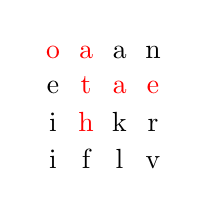
\begin{tikzpicture}
\matrix [matrix of nodes]
{ 
\textcolor{red}{o} & \textcolor{red}{a} & a & n\\
e & \textcolor{red}{t} & \textcolor{red}{a} & \textcolor{red}{e}\\
i & \textcolor{red}{h} & k & r\\
i & f & l & v\\
};
\end{tikzpicture}
\end{figure} 
\textbf{Output}: [\texttt{eat}, \texttt{oath}]
\end{flushleft}
\paragraph{Note:}
\begin{itemize}
\item You may assume that all inputs are consist of lowercase letters a--z.
\end{itemize}
\subsection{DFS + Trie}
\begin{CJK*}{UTF8}{gbsn}
\begin{itemize}
\item Trie的node数据结构中需要放入所加入的word。
\item 为了避免使用额外的数组来判断$B$中某个位置是否访问过,可以先把该位置上的字符替换为除了a -- z之外的其他字符。然后DFS函数末尾再换回该位置上的原字符。
\begin{lstlisting}[style=customc]
void DFS(B, r, c)
{
 	char letter = B[r][c]; //Save to letter
 	B[r][c] = '#'; //set to a special character
 	....
 	B[r][c] = letter; //Reset to original letter
}
\end{lstlisting}
\item 如果当前Trie node的word存在,那么除了把这个word加入到返回结果中,可以把这个word置为empty string。这样避免了在返回结果中出现重复的word。
\end{itemize}
\end{CJK*}
\setcounter{algorithm}{0}
\begin{algorithm}[H]
\caption{DFS Plus Trie}
\begin{algorithmic}[1]
\State $\star$ $B$ has dimension $R\times C$. $W$ has length $L$
\Procedure{FindWords}{$B, R, C, W, L$}
\State $\star$ Add each word from $W$ into Trie
\State $\star$ Iterate over all elements in $B$
\State $\omega:=\emptyset$ \Comment The found words
\For{$r:=0\to R-1$} \Comment Row
\For{$c:=0\to C-1$} \Comment Column
\State $\star$ Call helper function \texttt{DFS} to find word in $W$
\State \Call{DFS}{$B, t, r, c, \omega$}
\EndFor
\EndFor
\State \Return $\omega$
\EndProcedure
\end{algorithmic}
\end{algorithm}
Function \texttt{DFS} have 5 inputs which are
\begin{itemize}
\item $B$: The input board
\item $r$ and $c$: The start position to do DFS
\item $t$: The root of \textbf{Trie}
\item $\omega$: The found words
\end{itemize}
\begin{algorithm}[H]
\caption{Helper Function}
\begin{algorithmic}[1]
\Function{DFS}{$B,r,c,t,\omega$}
\If{$B[r][c]$ is not in $t$'s children}
\State \Return
\EndIf
\State $\star$ Update $t$ as $t$'s child in index corresponding to $B[r][c]$
\If{$t$ has a non-empty \texttt{word} member which is in the dictionary}
\State $\star$ Add $t$'s \texttt{word} memeber to $\omega$ and reset $t$'s \texttt{word} to empty
\EndIf
\algstore{212algo}
\end{algorithmic}
\end{algorithm}
\begin{algorithm}[H]
\begin{algorithmic}[1]
\algrestore{212algo}
\State $x:=B[r][c]$ \Comment Save $B[r][c]$ to $x$
\State Set $B[r][c]$ to a special character $\pi$ other than a--z.
\State $\star$ Move one unit in 4 directions. Each move will get a new position $(r_1, c_1)$
\If{$(r_1, c_1)$ is inside $B$ and $B[r_1][c_1]\neq \pi$}
\State \Call{DFS}{$B, r_1, c_1, t, \omega$} \Comment Continue DFS from $(r_1,c_1)$
\EndIf
\State $B[r][c]\gets x$ \Comment Restore $B[r][c]$ as its original letter
\EndFunction
\end{algorithmic}
\end{algorithm}
\setcounter{lstlisting}{0}
\begin{lstlisting}[style=customc, caption={DFS And Trie}]
class Solution
{
	//Trie Node defintion
    struct Node
    {
        vector<Node*> siblings;
		// A little change: save added word
        string word;
        Node()
            : siblings( 26, nullptr )
        {}

    };

public:
    vector<string> findWords( vector<vector<char>>& board, vector<string>& words )
    {

        for( const auto& w : words )
        {
            addWord( w );
        }

        int rows = static_cast<int>( board.size() );
        int cols = static_cast<int>( board[0].size() );

        vector<string> ans;
        ans.reserve( words.size() );

        for( int r = 0; r < rows; ++r )
        {
            for( int c = 0; c < cols; ++c )
            {
                dfs( board, m_root, r, c, ans );
            }
        }

        return ans;
    }

    void dfs( vector<vector<char>>& G, Node* node, int r, int c, vector<string>& ans )
    {
        int rows = static_cast<int>( G.size() );
        int cols = static_cast<int>( G[0].size() );

        int index = G[r][c] - 'a';

        if( node->siblings[index] == nullptr )
        {
            return;
        }

        node = node->siblings[index];

		//Save original letter 
        auto letter = G[r][c];
		//indicate this position has been visited
        G[r][c] = '#'; 

        if( !node->word.empty() )
        {
            ans.emplace_back( node->word );
			//Avoid duplicate words in ans
            node->word.clear();
        }

        for( const auto& d : m_dirs )
        {
            int nr = r + d.first;
            int nc = c + d.second;

            if( ( nr >= 0 ) && ( nr < rows ) && ( nc >= 0 ) && ( nc < cols ) && ( G[nr][nc] != '#' ) )
            {
                dfs( G, node, nr, nc, ans );
            }
        }

		//reset to original letter
        G[r][c] = letter; 
    }

    void addWord( const string& word )
    {
        auto node = m_root;

        for( auto c : word )
        {
            int i = c - 'a';
            if( node->siblings[i] == nullptr )
            {
                node->siblings[i] = new Node();
            }

            node = node->siblings[i];
        }

		//put word into the node
        node->word = word;
    }

    Node* m_root = new Node();
	
	// The offset in 4 directions
    vector<pair<int, int>> m_dirs =
    {
        {-1, 0}, {1, 0}, {0, -1}, {0, 1}
    };
};
\end{lstlisting}
%\section{213 --- House Robber II}
You are a professional robber planning to rob houses along a street. Each house has a certain amount of money stashed. All houses at this place are \textbf{arranged in a circle}. That means the first house is the neighbor of the last one. Meanwhile, adjacent houses have security system connected and it will automatically contact the police \textbf{if two adjacent houses were broken into on the same night}.
\par
Given a list of non-negative integers $A$ representing the amount of money of each house, determine the maximum amount of money you can rob tonight without alerting the police.
\paragraph{Example 1:}
\begin{flushleft}
\textbf{Input}: $[2,3,2]$
\\
\textbf{Output}: 3
\\
\textbf{Explanation}: 
\\
You cannot rob house 1 (money = 2) and then rob house 3 (money = 2), because they are adjacent houses.
\end{flushleft}
\textbf{Example 2:}
\begin{flushleft}
\textbf{Input}: $[1,2,3,1]$
\\
\textbf{Output}: 4
\\
\textbf{Explanation}: 
\\
Rob house 1 (money = 1) and then rob house 3 (money = 3). Total amount you can rob $= 1 + 3 = 4$.
\end{flushleft}
\subsection{Dynamic Programming}
\begin{CJK*}{UTF8}{gbsn}
和199相类似的题,但是由于$A[0]$和$A[L-1]$是相邻的($L$是$A$的长度),因此实际上问题其实就是求出下列两种情况的最大值
\begin{itemize}
\item 从$A[0]$到$A[L-2]$得到的最大值
\item 从$A[1]$到$A[L-1]$得到的最大值
\end{itemize}
\end{CJK*}
\setcounter{algorithm}{0}
\begin{algorithm}[H]
\caption{Dynamic Programming}
\begin{algorithmic}[1]
\Procedure{Rob}{$A, L$}
\If{$L = 0$} \Comment Empty array
\State \Return 0
\EndIf
\State $\star$ Get the maximum amount from $A[0]$ to $A[L-2]$
\State $x:=A[0]$ \Comment The maximum amount if $A[i]$ is selected
\State $y:=0$ \Comment The maximum amount if $A[i]$ is not selected
\For{$i:=0\to L-2$}
\State $x_0:=x$
\State $y_0:=y$
\State $x\gets \max(x_0, y_0+A[i])$ \Comment $A[i]$ is selected, so $A[i-1]$ cannot be selected
\State $y\gets \max(x_0, y_0)$ \Comment $A[i]$ is not selected, so $A[i-1]$ can be selected or not
\EndFor
\State $z_0:=\max(x,y)$ \Comment The maximum amount from $A[0]$ to $A[L-2]$
\If{$L=1$} \Comment Only one element in $A$
\State \Return $z_0$
\EndIf
\State $\star$ Get the maximum amount from $A[1]$ to $A[L-1]$
\State $x:=A[1]$ \Comment The maximum amount if $A[i]$ is selected
\State $y:=0$ \Comment The maximum amount if $A[i]$ is not selected
\For{$i:=1\to L-1$}
\State $x_0:=x$
\State $y_0:=y$
\State $x\gets \max(x_0, y_0+A[i])$ \Comment $A[i]$ is selected, so $A[i-1]$ cannot be selected
\State $y\gets \max(x_0, y_0)$ \Comment $A[i]$ is not selected, so $A[i-1]$ can be selected or not
\EndFor
\State $z_1:=\max(x,y)$ \Comment The maximum amount from $A[1]$ to $A[L-1]$
\State \Return $\max(z_0, z_1)$
\EndProcedure
\end{algorithmic}
\end{algorithm}
\setcounter{lstlisting}{0}
\begin{lstlisting}[style=customc, caption={Dynamic Programming}]
int rob( vector<int>& nums )
{
    if( nums.empty() )
    {
        return 0;
    }

	// Process from A[0] to A[L-2]
    int x = nums[0];
    int y = 0;

    int L = static_cast<int>( nums.size() );

    for( int i = 1; i < L - 1; ++i )
    {
        int last_x = x;
        int last_y = y;

        x = ( max )( last_x, last_y + nums[i] );
        y = ( max )( last_x, last_y );
    }

    int ans = ( max )( x, y );

	// Process from A[1] to A[L-1]
    if( nums.size() < 2 )
    {
        return ans;
    }

    x = nums[1];
    y = 0;

    for( int i = 2; i < L; ++i )
    {
        int last_x = x;
        int last_y = y;

        x = ( max )( last_x, last_y + nums[i] );
        y = ( max )( last_x, last_y );
    }

    int t = ( max )( x, y );

    ans = ( max )( ans, t );

    return ans;
}
\end{lstlisting}

%\section{214 --- Shortest Palindrome}
Given a string $s$, you are allowed to convert it to a palindrome by adding characters in front of it. Find and return the shortest palindrome you can find by performing this transformation.
\paragraph{Example 1:}
\begin{flushleft}
\textbf{Input}: \texttt{aacecaaa}
\\
\textbf{Output}: \texttt{aaacecaaa}
\end{flushleft}
\paragraph{Example 2:}
\begin{flushleft}
\textbf{Input}: \texttt{abcd}
\\
\textbf{Output}: \texttt{dcbabcd}
\end{flushleft}
\subsection{KMP}
由于只能在$s$的最前面插入字符,因此首先找到从$s[0]$开始最长的palindrome substring,假设其长度为$x$,即$s[0,x-1]$是palindrome。然后copy $s[x,l-1]$($l$是$s$的长度)到$y$,对$y$进行反转,然后$y+s$就是所求的最小长度的palindrome了。
\par
例如,$s=\texttt{abcbabcab}$. 从$s[0]$开始最长的palindrome substring 是\texttt{abcba}, 而剩下的部分是\texttt{bcab},其反转后为\texttt{bacb}. 因此,产生的最小长度palindrome即为$\texttt{bacb} + s = \texttt{bacbabcbabcab}$
\par
普通的方法所产生的时间复杂度为$O(n^2)$。因此需要KMP来进行优化。

\subsubsection{KMP Overview}
\textbf{KMP} is a string matching algorithm that runs in $O(n+m)$ times, where $n$ and $m$ are sizes of the text and string to be searched respectively. The key component of \textbf{KMP} is the failure function lookup table, say $f(s)$. The purpose of the lookup table is to store the length of the proper prefix of the string $b_{1}b_{2}\ldots b_{s}$ that is also a suffix of $b_{1}b_{2}\ldots b_{s}$
\par
This table is important because if we are trying to match a text string for $b_{1}b_{2}\ldots b_{n}$ and we have matched the first $s$ positions, but when we fail, then the value of lookup table for $s$ is the longest prefix of $b_{1}b_{2}\ldots b_{n}$ that could possibly match the text string up to the point we are at. Thus, we don't need to start all over again, and can resume searching from the matching prefix.
\par
The algorithm to generate the lookup table is easy and inutitive, as given below:
\setcounter{algorithm}{0}
\begin{algorithm}[H]
\caption{KMP Lookup Table Generation}
\begin{algorithmic}[1]
\Procedure{KMPTable}{$b, n$}
\State $\star$ Initialize an array $f$ with length $n$
\State $f[0]\gets 0$
\For{$i:=1 \to n-1$}
\State $t:=f[i-1]$
\While{$t > 0$ \textbf{and} $b[i]\neq b[t]$}
\State $t\gets f[t-1]$
\EndWhile
\If{$b[i]=b[t]$}
\State $t\gets t+1$
\EndIf
\State $f[i]\gets t$
\EndFor
\EndProcedure
\end{algorithmic}
\end{algorithm}
\begin{itemize}
\item First set $f(0)=0$ since no proper prefix is available.
\item Next, iterate over $i$ from $1$ to $n-1$:
\begin{itemize}
\item Set $t=f(i-1)$
\item While $t>0$ and letter at $i$ doesn't match the letter at $t$ position, set $t=f(t)$, which essentially means that we have problem matching and must consider a shorter prefix, which will be $b_{f(t-1)}$, until we find a match or t becomes 0.
\item If $b[i]=b[t]$, increments $t$ 
\item Set $f[i]\gets t$
\end{itemize}
\end{itemize}
The lookup table generation is as illustrated below:
\par
Take a string \texttt{cacacabc} as an example:
\par
At start No proper prefix $f[0]=0$
\begin{figure}[H]
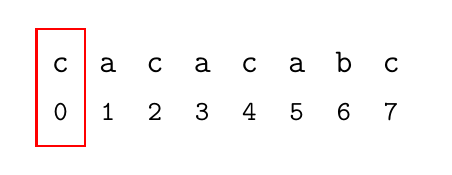
\begin{tikzpicture}
\matrix(m)[nodes={minimum size=6mm}, column sep= 0mm, anchor=base]
{
\node(1){\large \texttt{c}}; & \node(2){\large \texttt{a}};
& \node(3){\large \texttt{c}};& \node(4){\large \texttt{a}};
& \node(5){\large \texttt{c}};& \node(6){\large \texttt{a}};
& \node(7){\large \texttt{b}};& \node(8){\large \texttt{c}};\\
\node(21){\texttt{0}}; & \node(22){\texttt{1}};
& \node(23){\texttt{2}};& \node(24){\texttt{3}};
& \node(25){\texttt{4}};& \node(26){\texttt{5}};
& \node(27){\texttt{6}};& \node(28){\texttt{7}};\\
};
\draw[red, line width=0.3mm] (m.north west -| 1.west) rectangle (m.south west -| 1.east);
\end{tikzpicture}
\end{figure}
\begin{enumerate}
\item $i=1$, $t\gets f[0]$ so $t=0$
\begin{figure}[H]
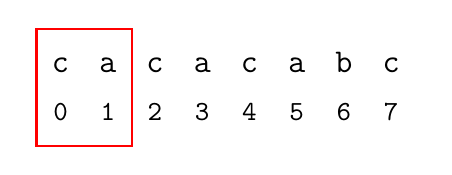
\begin{tikzpicture}
\matrix(m)[nodes={minimum size=6mm}, column sep= 0mm, anchor=base]
{
\node(1){\large \texttt{c}}; & \node(2){\large \texttt{a}};
& \node(3){\large \texttt{c}};& \node(4){\large \texttt{a}};
& \node(5){\large \texttt{c}};& \node(6){\large \texttt{a}};
& \node(7){\large \texttt{b}};& \node(8){\large \texttt{c}};\\
\node(21){\texttt{0}}; & \node(22){\texttt{1}};
& \node(23){\texttt{2}};& \node(24){\texttt{3}};
& \node(25){\texttt{4}};& \node(26){\texttt{5}};
& \node(27){\texttt{6}};& \node(28){\texttt{7}};\\
};
\draw[red, line width=0.3mm] (m.north west -| 1.west) rectangle (m.south west -| 2.east);
\end{tikzpicture}
\end{figure}
No proper prefix equal to suffix yet. Therefore $f[1] \gets 0$.
\item $i=2$, $t\gets f[1]$ so $t=0$, but $b[2] = b[0] = c \Longrightarrow t\gets t+1$
\begin{figure}[H]
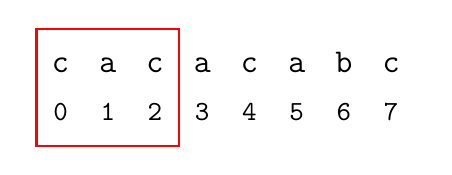
\begin{tikzpicture}
\matrix(m)[nodes={minimum size=6mm}, column sep= 0mm, anchor=base]
{
\node(1){\large \texttt{c}}; & \node(2){\large \texttt{a}};
& \node(3){\large \texttt{c}};& \node(4){\large \texttt{a}};
& \node(5){\large \texttt{c}};& \node(6){\large \texttt{a}};
& \node(7){\large \texttt{b}};& \node(8){\large \texttt{c}};\\
\node(21){\texttt{0}}; & \node(22){\texttt{1}};
& \node(23){\texttt{2}};& \node(24){\texttt{3}};
& \node(25){\texttt{4}};& \node(26){\texttt{5}};
& \node(27){\texttt{6}};& \node(28){\texttt{7}};\\
};
\draw[red, line width=0.3mm] (m.north west -| 1.west) rectangle (m.south west -| 3.east);
\end{tikzpicture}
\end{figure}
Suffix and prefix both are {\LARGE \texttt{c}}. Hence $f[2]\gets t=1$

\item $i=3$, $t\gets f[2]$ so $t=1$, but $b[3] = b[1] = a \Longrightarrow t\gets t+1$
\begin{figure}[H]
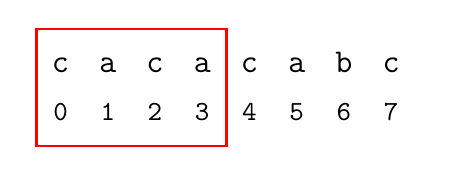
\begin{tikzpicture}
\matrix(m)[nodes={minimum size=6mm}, column sep= 0mm, anchor=base]
{
\node(1){\large \texttt{c}}; & \node(2){\large \texttt{a}};
& \node(3){\large \texttt{c}};& \node(4){\large \texttt{a}};
& \node(5){\large \texttt{c}};& \node(6){\large \texttt{a}};
& \node(7){\large \texttt{b}};& \node(8){\large \texttt{c}};\\
\node(21){\texttt{0}}; & \node(22){\texttt{1}};
& \node(23){\texttt{2}};& \node(24){\texttt{3}};
& \node(25){\texttt{4}};& \node(26){\texttt{5}};
& \node(27){\texttt{6}};& \node(28){\texttt{7}};\\
};
\draw[red, line width=0.3mm] (m.north west -| 1.west) rectangle (m.south west -| 4.east);
\end{tikzpicture}
\end{figure}
Suffix and prefix both are {\LARGE \texttt{ca}}. Hence $f[3]\gets t=2$

\item $i=4$, $t\gets f[3]$ so $t=2$, but $b[4] = b[2] = c \Longrightarrow t\gets t+1$,
\begin{figure}[H]
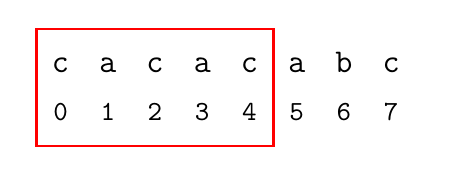
\begin{tikzpicture}
\matrix(m)[nodes={minimum size=6mm}, column sep= 0mm, anchor=base]
{
\node(1){\large \texttt{c}}; & \node(2){\large \texttt{a}};
& \node(3){\large \texttt{c}};& \node(4){\large \texttt{a}};
& \node(5){\large \texttt{c}};& \node(6){\large \texttt{a}};
& \node(7){\large \texttt{b}};& \node(8){\large \texttt{c}};\\
\node(21){\texttt{0}}; & \node(22){\texttt{1}};
& \node(23){\texttt{2}};& \node(24){\texttt{3}};
& \node(25){\texttt{4}};& \node(26){\texttt{5}};
& \node(27){\texttt{6}};& \node(28){\texttt{7}};\\
};
\draw[red, line width=0.3mm] (m.north west -| 1.west) rectangle (m.south west -| 5.east);
\end{tikzpicture}
\end{figure}
Suffix and prefix both are {\LARGE \texttt{cac}}. Hence $f[4]\gets t=3$

\item $i=5$, $t\gets f[4]$ so $t=3$, but $b[5] = b[3] = a \Longrightarrow t\gets t+1$,
\begin{figure}[H]
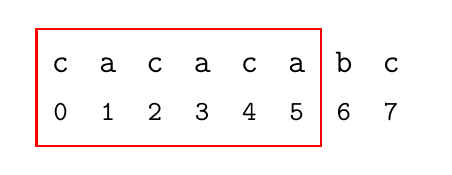
\begin{tikzpicture}
\matrix(m)[nodes={minimum size=6mm}, column sep= 0mm, anchor=base]
{
\node(1){\large \texttt{c}}; & \node(2){\large \texttt{a}};
& \node(3){\large \texttt{c}};& \node(4){\large \texttt{a}};
& \node(5){\large \texttt{c}};& \node(6){\large \texttt{a}};
& \node(7){\large \texttt{b}};& \node(8){\large \texttt{c}};\\
\node(21){\texttt{0}}; & \node(22){\texttt{1}};
& \node(23){\texttt{2}};& \node(24){\texttt{3}};
& \node(25){\texttt{4}};& \node(26){\texttt{5}};
& \node(27){\texttt{6}};& \node(28){\texttt{7}};\\
};
\draw[red, line width=0.3mm] (m.north west -| 1.west) rectangle (m.south west -| 6.east);
\end{tikzpicture}
\end{figure}
Suffix and prefix both are {\LARGE \texttt{caca}}. Hence $f[5]\gets t=4$

\item $i=6$, $t=f[5]$ so $t=4$, now $b[6]\neq b[4] \Longrightarrow t\gets f[t-1]$ which leads to $t\gets f[3]=2$. However, $b[6]\neq b[2] \Longleftrightarrow t\gets f[t-1]$ which further leads to $t\gets f[1]$. Now $t$ is updated to zero.
\begin{figure}[H]
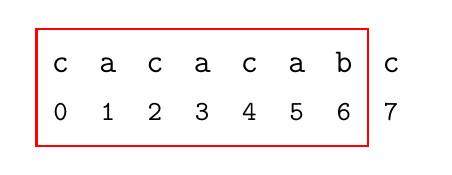
\begin{tikzpicture}
\matrix(m)[nodes={minimum size=6mm}, column sep= 0mm, anchor=base]
{
\node(1){\large \texttt{c}}; & \node(2){\large \texttt{a}};
& \node(3){\large \texttt{c}};& \node(4){\large \texttt{a}};
& \node(5){\large \texttt{c}};& \node(6){\large \texttt{a}};
& \node(7){\large \texttt{b}};& \node(8){\large \texttt{c}};\\
\node(21){\texttt{0}}; & \node(22){\texttt{1}};
& \node(23){\texttt{2}};& \node(24){\texttt{3}};
& \node(25){\texttt{4}};& \node(26){\texttt{5}};
& \node(27){\texttt{6}};& \node(28){\texttt{7}};\\
};
\draw[red, line width=0.3mm] (m.north west -| 1.west) rectangle (m.south west -| 7.east);
\end{tikzpicture}
\end{figure}
No proper prefix equal to suffix. Hence $f[6]\gets t=0$

\item $i=7$, $t=f[6]$ so $t=0$, but $b[7] = b[0]\Longrightarrow t\gets t+1$
\begin{figure}[H]
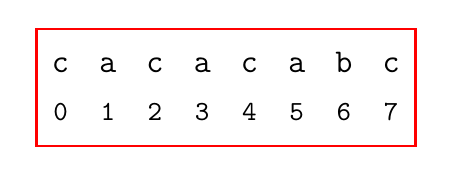
\begin{tikzpicture}
\matrix(m)[nodes={minimum size=6mm}, column sep= 0mm, anchor=base]
{
\node(1){\large \texttt{c}}; & \node(2){\large \texttt{a}};
& \node(3){\large \texttt{c}};& \node(4){\large \texttt{a}};
& \node(5){\large \texttt{c}};& \node(6){\large \texttt{a}};
& \node(7){\large \texttt{b}};& \node(8){\large \texttt{c}};\\
\node(21){\texttt{0}}; & \node(22){\texttt{1}};
& \node(23){\texttt{2}};& \node(24){\texttt{3}};
& \node(25){\texttt{4}};& \node(26){\texttt{5}};
& \node(27){\texttt{6}};& \node(28){\texttt{7}};\\
};
\draw[red, line width=0.3mm] (m.north west -| 1.west) rectangle (m.south west -| 8.east);
\end{tikzpicture}
\end{figure}
Suffix and prefix both are {\LARGE \texttt{c}}. Hence $f[7]\gets t=1$
\end{enumerate}
The final table is:
\begin{table}[H]
\begin{tabular}{|c|l|l|l|l|l|l|l|l|}
\hline
$i$    & 0 & 1 & 2 & 3 & 4 & 5 & 6 & 7 \\ \hline
$f(i)$ & 0 & 0 & 1 & 2 & 3 & 4 & 0 & 1 \\ \hline
\end{tabular}
\end{table}

\subsubsection{Apply KMP}
如果把$s$进行反转,然后append在$s$后,这样问题就转变成求最长的proper prefix which is equal to suffix。这样就需要KMP lookup table了。
\begin{itemize}
\item 将$s$ reverse 为 $\hat{s}$
\item 在$s$和$\hat{s}$中间加入一个特殊字符 t, 比如\$。形成一个新的string $x$,即$x=s+t+\hat{s}$。这个$t$是必须的,比如\texttt{aaaa},如果不加$t$,$x=\texttt{aaaaaaaa}$,那么最长的prefix就是\texttt{aaaaaaa},长度为7。(注意,prefix是不包含整个string的)。
\item 生成$x$的KMP lookup table $f$。那么$f[l_t-1]$的长度就是$t$最长的prefix与suffix相等的substring的长度。于是$s$中反转的部分即为$\hat{s}[0, l_s-f[l_t-1]$
\item $\hat{s}[0, l\_s-f[l\_t-1]] + s$即为所能生成的最小长度的palindrome string。
\end{itemize}
\setcounter{algorithm}{0}
\begin{algorithm}[H]
\caption{KMP Lookup Table}
\begin{algorithmic}[1]
\Procedure{ShortestPalindrome}{$S, L$}
\State $\star$ Reverse $S$ as $\hat{S}$
\State $\star$ Generate string $x=S + \omega + \hat{S}$ where $\omega$ is a special character
\State $\star$ Initialize KMP lookup table $f$ whose length is $|x|$
\State $\star$ Generate KMP lookup table for string $x$
\State $f[0]=0$
\For{$i:=1 \to l_x-1$}
\State $t:=f[i-1]$
\While{$t> 0$ \textbf{and} $x[i]\neq x[t]$}
\State $t\gets f[t-1]$
\EndWhile
\If{$x[i]=x[t]$}
\State $t\gets t+1$
\EndIf
\State $f[i]\gets t$
\EndFor
\State $\star$ Suppose $y$ is the part of $S$ after the longest palindrome substring from $S[0]$
\State $\star$ $y:=S[f[l_x-1], L-1]$.
\State $\star$ Since $y$ need to be reversed to $\hat{y}$, actually $\hat{y}:=\hat{S}[0, L - f[l_x-1]]$
\State \Return $\hat{y} + S$
\EndProcedure
\end{algorithmic}
\end{algorithm}
\setcounter{lstlisting}{0}
\begin{lstlisting}[style=customc, caption={KMP Table}]
string shortestPalindrome( string s )
{
    string r;
    r = s;

	//reverse s
    reverse( r.begin(), r.end() );

    string x;
    //reserve x memory to avoid memory allocation
    x.reserve( s.size() + r.size() + 1 );

    x = s;
    x.push_back( '*' );
    x += r;

	//Generate KMP table
    vector<int> f( x.size(), 0 );

    for( size_t i = 1; i < x.size(); ++i )
    {
        int t = f[i - 1];

        while( ( t > 0 ) && ( x[t] != x[i] ) )
        {
            t = f[t - 1];
        }

        if( x[t] == x[i] )
        {
            ++t;
        }

        f[i] = t;
    }

    string ans = r.substr( 0, s.size() - f.back() );
    ans += s;

    return ans;

}
\end{lstlisting}

%\section{215 --- Kth Largest Element in an Array}
Find the $k$th largest element in an unsorted array. Note that it is the $k$th largest element in the sorted order, not the $k$th distinct element.
\paragraph{Example 1:}
\begin{flushleft}
\textbf{Input}: $[3,2,1,5,6,4]$ and $k = 2$
\\
\textbf{Output}: 5
\end{flushleft}
\paragraph{Example 2:}
\begin{flushleft}
\textbf{Input}: $[3,2,3,1,2,4,5,5,6]$ and $k = 4$
\\
\textbf{Output}: 4
\end{flushleft}
\paragraph{Note:} 
\begin{itemize}
\item You may assume $k$ is always valid, $1 \leq k \leq $ array's length.
\end{itemize}
\subsection{Quick Select Algorithm}
In \textbf{quick sort} algorithm, there is a subprocedure called \textbf{partition} that can, in linear time, group an array (ranging from indices $l$ to $r$) into two parts: those less than a certain element, and those greater than or equal to the element. Here is pseudocode that performs a partition about the element $A[p]$

Like \textbf{Lomuto}'s partition scheme, \textbf{Hoare}'s partitioning also would cause \textbf{quick sort} to degrade to $O(n^2)$ for already sorted input, if the pivot was chosen as the \textbf{first} or the \textbf{last} element. With the \textbf{middle} element as the \textbf{pivot}, however, sorted data results with (almost) \textbf{no swaps} in equally sized partitions leading to best case behavior of quick sort, i.e. $O(n \log n)$. Like others, \textbf{Hoare}'s partitioning does not produce a stable sort.

Note that in this scheme, the pivot's final location is not necessarily at the index that was returned, and the next two segments that the main algorithm recurs on are $[l, p]$ and $[p+1, r]$ as opposed to $[l, p-1]$ and $[p+1, r]$ as in \textbf{Lomuto}'s scheme. However, the partitioning algorithm guarantees $l\geq p < r$ which implies both resulting partitions are non-empty, hence there's no risk of infinite recursion.

Back to the quick selection algorithm: In \textbf{quick sort}, we recursively sort both branches, leading to best-case $O(n \log n)$ time. However, when doing \textbf{selection}, we already know which partition our desired element lies in, since the pivot is in its final sorted position, with all those preceding it in an unsorted order and all those following it in an unsorted order. Therefore, a single recursive call locates the desired element in the correct partition, and we build upon this for \textbf{quick select}:


有一点需要注意,题目要求的是$k$th largest,而上述算法则是$k$th smallest,因此需要转换一下,求$k$th largest 实际上等价于求 $(L-k)$th smallest ($L$是原数组的长度)。

另外,Horae partition schema由于返回的不一定是 pivot的最终位置,因此在quick select中不太适合。

\setcounter{lstlisting}{0}
\begin{lstlisting}[style=customc, caption={Quick Select}]
class Solution
{
public:
    int findKthLargest( vector<int>& nums, int k )
    {
        int L = static_cast<int>( nums.size() );

		//Kth largest is L-K smallest
        return quickselect( nums, 0, L - 1, L - k );
    }

    int partition( vector<int>& A, int l, int r, int p )
    {
        int x = A[p];
        swap( A[p], A[r] );

        int alpha = l;

        for( int i = l; i < r; ++i )
        {
            if( A[i] < x )
            {
                swap( A[i], A[alpha] );
                ++alpha;
            }
        }

        swap( A[alpha], A[r] );

        return alpha;
    }

    int quickselect( vector<int>& A, int l, int r, int k )
    {
        while( true )
        {
            if( l == r )
            {
                return A[l];
            }

            int p = ( l + r ) / 2;
            p = partition( A, l, r, p );

            if( k == p )
            {
                return A[p];
            }

			// The kth smallest element is left of p
            if( k < p )
            {
                r = p - 1;
            }
            // The kth smallest element is right of p
            else
            {
                l = p + 1;
            }
        }

    }
};
\end{lstlisting}

 

%\section{216 --- Combination Sum III}
Find all possible combinations of $k$ numbers that add up to a number $n$, given that only numbers from 1 to 9 can be used and each combination should be a unique set of numbers.
\paragraph{Note:}
\begin{itemize}
\item All numbers will be positive integers.
\item The solution set must not contain duplicate combinations.
\end{itemize}
\paragraph{Example 1:}
\begin{flushleft}
\textbf{Input}: $k = 3$, $n = 7$
\\
\textbf{Output}: 
\\
\fcj{[[1,2,4]]}
\end{flushleft}
\paragraph{Example 2:}
\begin{flushleft}
\textbf{Input}: $k = 3$, $n = 9$
\\
\textbf{Output}: 
\\
$[[1,2,6], [1,3,5], [2,3,4]]$
\end{flushleft}
\subsection{Backtracking Recursion}
\begin{itemize}
\item 递归生成array
\item 每个小于$n$的数,先加入到当前array中,然后继续递归,结束后移除这个加入的数,然后前进到下一个数
\item 为保证不出现重复数字,递归函数应当有一个参数来表示当前搜索到哪个数字了。
\end{itemize}

\setcounter{lstlisting}{0}
\begin{lstlisting}[style=customc, caption={Backtracking}]
vector<vector<int>> combinationSum3( int k, int n )
{
    vector<vector<int>> ans;
    vector<int> v;

    dfs( n, k, 0, 1, v, ans );
	
    return ans;
}
//n: the count of numbers in v
//k: the required count of numbers
//sum: current sum of numbers in v
//start: The start number that will check
//v: The current array
void dfs( int n, int k, int sum, int start, vector<int>& v, vector<vector<int>>& ans )
{
    if( k == 0 )
    {
        if( sum == n )
        {
            ans.emplace_back( v.begin(), v.end() );
        }

        return;
    }

    for( int i = start; i <= 9; ++i )
    {
        if( i < n )
        {
			//Add i to v
            v.push_back( i );
            dfs( n, k - 1, sum + i, i + 1, v, ans );
			//Remove i from v
            v.pop_back();
        }
    }
}
\end{lstlisting}
%\section{217 --- Contains Duplicate}
Given an array of integers $A$, find if the array contains any duplicates.
\par
Your function should return \texttt{true} if any value appears at least twice in the array, and it should return \texttt{false} if every element is distinct.

\paragraph{Example 1:}
\begin{flushleft}
\textbf{Input}: $[1,2,3,1]$
\\
\textbf{Output}: \texttt{true}
\end{flushleft}

\paragraph{Example 2:}
\begin{flushleft}
\textbf{Input}: $[1,2,3,4]$
\\
\textbf{Output}: \texttt{false}
\end{flushleft}

\paragraph{Example 3:}
\begin{flushleft}
\textbf{Input}: $[1,1,1,3,3,4,3,2,4,2]$
\\
\textbf{Output}: \texttt{true}
\end{flushleft}
\subsection{Hash Set}
Utilize a hash set to find the duplicate number

%\section{218 --- The Skyline Problem}
A city's skyline is the outer contour of the silhouette formed by all the buildings in that city when viewed from a distance. Now suppose you are given \textbf{the locations and height of all the buildings} as shown on a cityscape photo (Figure A), write a program to \textbf{output the skyline} formed by these buildings collectively (Figure B).
\renewcommand{\thesubfigure}{\Alph{subfigure}}
\begin{figure}[H]
\begin{subfigure}[b]{8cm}
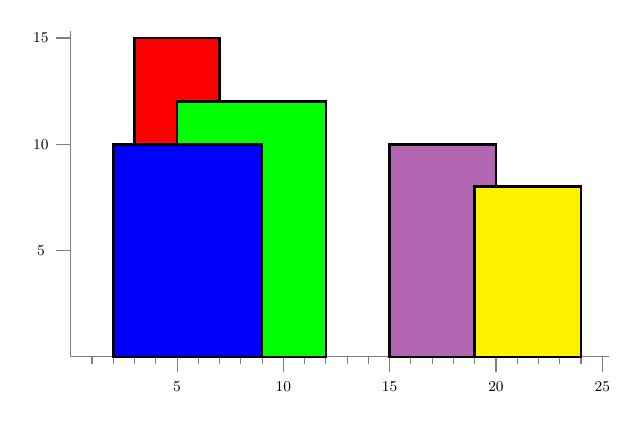
\begin{tikzpicture}[scale=0.9,every node/.style={scale=0.6}]
\draw[color=black!50!] (0,0) -- (7.6,0);
\draw[color=black!50!] (0,0) -- (0, 4.6);
\foreach \x in {0.3,0.6,...,7.5}
\draw[color=black!50!] (\x, -3pt) -- (\x, 0);
\foreach \x in {5,10,...,25}
{
\draw[color=black!50!] (\x*0.3, -6pt) -- (\x*0.3, 0);
\node at (\x*0.3,-12pt) {\small \x};
}
\foreach \y in {5,10,...,15}
{
\draw[color=black!50!] (-6pt,\y*0.3) -- (0, \y*0.3);
\node at (-12pt, \y*0.3) {\small \y};
}
\filldraw[draw=black, line width=1pt, fill=red] (0.9, 0) rectangle (2.1,4.5);
\filldraw[draw=black, line width=1pt, fill=green] (1.5,0) rectangle (3.6,3.6);
\filldraw[draw=black, line width=1pt, fill=blue] (0.6, 0) rectangle (2.7,3.0);
\filldraw[draw=black, line width=1pt, fill=violet!60!white] (4.5, 0) rectangle (6,3);
\filldraw[draw=black, line width=1pt, fill=yellow] (5.7, 0) rectangle (7.2,2.4);
\end{tikzpicture}
\caption{Buildings}
\end{subfigure}
\begin{subfigure}[b]{8cm}
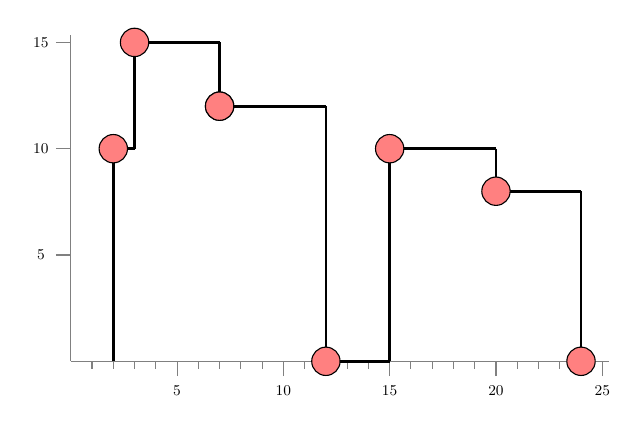
\begin{tikzpicture}[scale=0.9,every node/.style={scale=0.6}]
\draw[color=black!50!] (0,0) -- (7.6,0);
\draw[color=black!50!] (0,0) -- (0, 4.6);
\foreach \x in {0.3,0.6,...,7.5}
\draw[color=black!50!] (\x, -3pt) -- (\x, 0);
\foreach \x in {5,10,...,25}
{
\draw[color=black!50!] (\x*0.3, -6pt) -- (\x*0.3, 0);
\node at (\x*0.3,-12pt) {\small \x};
}
\foreach \y in {5,10,...,15}
{
\draw[color=black!50!] (-6pt,\y*0.3) -- (0, \y*0.3);
\node at (-12pt, \y*0.3) {\small \y};
}
\draw[line width=1pt] (0.6,0) -- (0.6,3);

\draw[line width=1pt] (0.6,3) -- (0.9,3);
\draw[line width=1pt] (0.9,3) -- (0.9,4.5);

\draw[line width=1pt] (0.9,4.5) -- (2.1,4.5);
\draw[line width=1pt] (2.1,4.5) -- (2.1,3.6);
\draw[line width=1pt] (2.1,3.6) -- (3.6,3.6);
\draw[line width=1pt] (3.6,3.6) -- (3.6, 0);
\draw[line width=1pt] (3.6,0) -- (4.5, 0);
\draw[line width=1pt] (4.5,0) -- (4.5, 3);
\draw[line width=1pt] (4.5,3) -- (6,3);
\draw[line width=1pt] (6,3) -- (6, 2.4);
\draw[line width=1pt] (6,2.4) -- (7.2, 2.4);
\draw[line width=1pt] (7.2,2.4) -- (7.2, 0);

\draw[fill=red!50!] (0.6,3) circle (2mm);
\draw[fill=red!50!] (0.9,4.5) circle (2mm);
\draw[fill=red!50!] (2.1,3.6) circle (2mm);
\draw[fill=red!50!] (3.6,0) circle (2mm);
\draw[fill=red!50!] (4.5,3) circle (2mm);
\draw[fill=red!50!] (2.1,3.6) circle (2mm);
\draw[fill=red!50!] (6,2.4) circle (2mm);
\draw[fill=red!50!] (7.2,0) circle (2mm);
\end{tikzpicture}
\caption{Silhouettes}
\end{subfigure}
\end{figure}
The geometric information of each building is represented by a triplet of integers $[L_i, R_i, H_i]$, where $L_i$ and $R_i$ are the $x$ coordinates of the left and right edge of the $i$th building, respectively, and $H_i$ is its height. It is guaranteed that $0 \leq L_i, R_i \leq$ \texttt{INT\_MAX}, $0 < H_i \leq$ \texttt{INT\_MAX}, and $R_i - L_i > 0$. You may assume all buildings are perfect rectangles grounded on an absolutely flat surface at height 0.
\par
For instance, the dimensions of all buildings in Figure A are recorded as:
$[2, 9, 10]$, $[3, 7, 15]$, $[5, 12, 12]$, $[15, 20, 10]$, $[19, 24, 8]$.
\par
The output is a list of \textit{key points} (red dots in Figure B) in the format of $[x_1,y_1]$, $[x_2, y_2]$, $[x_3, y_3]$, $\ldots$ that uniquely defines a skyline. A \textit{key point} is the left endpoint of a horizontal line segment. Note that the last key point, where the rightmost building ends, is merely used to mark the termination of the skyline, and always has zero height. Also, the ground in between any two adjacent buildings should be considered part of the skyline contour.
\par
For instance, the skyline in Figure B should be represented as:
$
[2, 10]$, $[3, 15]$, $[7, 12]$, $[12, 0]$, $[15 ,10]$, $[20, 8]$, $[24, 0]$

\paragraph{Notes:}
\begin{itemize}
    \item The number of buildings in any input list is guaranteed to be in the range $[0, 10000].$
    \item     The input list is already sorted in ascending order by the left $x$ position $L_i$.
    \item The output list must be sorted by the $x$ position.
    \item There must be no consecutive horizontal lines of equal height in the output skyline. For instance, $[2, 3]$, $[4, 5]$, $[7, 5]$, $[11, 5]$, $[12, 7]$ is not acceptable; the three lines of height 5 should be merged into one in the final output as such: $[2, 3], [4, 5], [12, 7]$
\end{itemize}
\subsection{Sorting}
\begin{itemize}
    \item 每个矩形的左上角和右上角是可能的轮廓变化点,称之为critical points。
    \item 如果相邻的两个矩形不重叠,左边矩形的右下角也是key point。
    \item 如果某个critical point处在一个矩形的左右边的范围内(即比较$x$坐标),那么这个轮廓变化点处的高度为这个点之前的高度和当前矩形的高度的最大值。
    \item 为了快速得到所有包含某个critical point的矩形高度的最大值,可以用一个maximum heap来进行排序。
\end{itemize}
算法大致过程如下:
\begin{enumerate}
    \item sort all the critical points. 
    \item 从左到右扫描上述排序后的critical points。如果遇到某个矩形的左边,就将这个矩形加入到heap中。如果遇到某个矩形的右边,就将这个矩形从heap中remove。
    \item 记录当前的最大高度,以及上一次的最大高度,如果发生改变,表示遇到了一个key point了。
    \item 最后,每次遇到critical point,将其高度更新为当前heap的top,即当前在heap中的所有矩形的高度的最大值。
\end{enumerate}
几个coding的技巧
\begin{itemize}
    \item 可以将矩形左边界的高度设置为负数,这样就很容易区分当前遇到的是矩形的左边界还是右边界了。
    \item 用\texttt{multiset}作为存放矩形高度的数据结构,因为\texttt{priority queue}不提供删除操作。
    \item 在遍历critical points之前,将0放入到heap中,因为最后的矩形的右下角总是要包含在key point中的。
\end{itemize}
\setcounter{algorithm}{0}
\begin{algorithm}[H]
\caption{Heap Based Sorting}
\begin{algorithmic}[1]
\Procedure{GetSkyline}{$B, L$}
\State $\star$ sort all left and right points in $B$
\State $H_0:=0$ \Comment Last maximum height
\For{Each sorted point $p$}
\If{$p$ is the left edge of a rectangle}
\State $\star$ Add $p$ to the heap
\Else
\State $\star$ Remove $p$ from the heap
\EndIf
\State $\star$ Get current maixmum height $H$ from the heap
\If{$H_0\neq H$} \Comment A key point is found
\State $\star$ Add $p$'s $x$ coordinate and $H$ into the result array
\State $H_0\gets H$ \Comment Update last maximum height
\EndIf
\EndFor
\State $\star$ Returns the result array
\EndProcedure
\end{algorithmic}
\end{algorithm}
\setcounter{lstlisting}{0}
\begin{lstlisting}[style=customc, caption={Sorting}]
public:
vector<pair<int, int>> getSkyline( vector<vector<int>>& buildings )
{

    set<pair<int, int>> pt_sets;

    for( const auto& b : buildings )
    {
        pt_sets.emplace( b[0], -b[2] );
        pt_sets.emplace( b[1], b[2] );
    }

    multiset<int> h_sets;
    h_sets.insert( 0 );

    int pre_h = 0;
    int cur_h = 0;

    vector<pair<int, int>> ans;

    for( const auto&pt : pt_sets )
    {
        if( pt.second < 0 )
        {
            h_sets.insert( -pt.second );
        }
        else
        {
            // h_sets.erase(pt.second) will remove all 
            // keys that equal to pt.second. It is not desired
            // since we want to remove only one element.
            h_sets.erase( h_sets.find( pt.second ) );
        }

        cur_h = *( h_sets.rbegin() );

        if( cur_h != pre_h )
        {
            ans.emplace_back( pt.first, cur_h );
            pre_h = cur_h;
        }
    }

    return ans;
}

\end{lstlisting}

%\section{219 --- Contains Duplicate II}
Given an array of integers $A$ and an integer $k$, find out whether there are two distinct indices $i$ and $j$ in the array such that $A[i] = A[j]$ and the absolute difference between $i$ and $j$ is at most $k$.
\paragraph{Example 1:}
\begin{flushleft}
\textbf{Input}: $A = [1,2,3,1]$, $k = 3$
\\
\textbf{Output}: \texttt{true}
\end{flushleft}

\paragraph{Example 2:}
\begin{flushleft}
\textbf{Input}: $A = [1,0,1,1]$, $k = 1$
\\
\textbf{Output}: \texttt{true}
\end{flushleft}
\paragraph{Example 3:}
\begin{flushleft}
\textbf{Input}: $A = [1,2,3,1,2,3]$, $k = 2$
\\
\textbf{Output}: \texttt{false}
\end{flushleft}
\subsection{Hash Table}
\begin{CJK*}{UTF8}{gbsn}
\begin{itemize}
    \item 由于遍历数组就是按照顺序遍历的,因此如果按照从小到大遍历,因此只需要判定当前index$i$与之前在hash table中的index$j$是否能存在$i-j\leq k$。
    \item 算法过程很直接,对于当前index对应的number$n$,如果在hash table中不存在,将$n$和对应的index插入到hash table中,如果存在,则按照上述分析进行比较,如果存在$i-j\leq k$,就直接返回\texttt{true},然后将$n$对应的index更新为$i$。
\end{itemize}
\end{CJK*}
\setcounter{algorithm}{0}
\begin{algorithm}[H]
\caption{Hash Table}
\begin{algorithmic}[1]
\Procedure{ContainsNearbyDuplicate}{$A, L$}
\State $\star$ Create an empty hash table $M$
\For{$i:=0\to L-1$}
\If{$A[i]$ is not in $M$}
\State $\star$ set $M[A[i]]:=i$
\Else
\State $j:=M[A[i]]$ \Comment Get the last index for number $A[i]$
\If{$i-j\leq k$}
\State \Return \texttt{true}
\Else
\State $M[A[i]]\gets j$ \Comment Update the index of $A[i]$
\EndIf
\EndIf
\EndFor
\State \Return \texttt{false}
\EndProcedure
\end{algorithmic}
\end{algorithm}

\setcounter{lstlisting}{0}

\begin{lstlisting}[style=customc, caption={Hash Table}]
bool containsNearbyDuplicate( vector<int>& nums, int k )
{

    unordered_map<int, int> m;

    int L = static_cast<int>( nums.size() );

    for( int i = 0; i < L; ++i )
    {
        auto it = m.find( nums[i] );

        if( it == m.end() )
        {
            m.emplace( nums[i], i );
        }
        else
        {
            if( i - it->second <= k )
            {
                return true;
            }

            it->second = i;
        }
    }

    return false;
}

\end{lstlisting}

%\section{220 --- Contains Duplicate III}

Given an array of integers $A$, find out whether there are two distinct indices $i$ and $j$ in the array such that the absolute difference between $A[i]$ and $A[j]$ is at most $t$ and the absolute difference between $i$ and $j$ is at most $k$.
\paragraph{Example 1}
\begin{flushleft}
\textbf{Input}: $A = [1,2,3,1]$, $k = 3$, $t = 0$
\\
\textbf{Output}: \texttt{true}
\end{flushleft}
\paragraph{Example 2:}
\begin{flushleft}
\textbf{Input}: $A = [1,0,1,1]$, $k = 1$, $t = 2$
\\
\textbf{Output}: \texttt{true}
\end{flushleft}
\paragraph{Example 3:}
\begin{flushleft}
\textbf{Input}: $A = [1,5,9,1,5,9]$, $k = 2$, $t = 3$
\\
\textbf{Output}: \texttt{false}
\end{flushleft}
\subsection{Tree Map}
\begin{itemize}
\item 对于index $i$,小于$i-k$的index对结果没有影响。
\item 需要找到在$[i-k, i]$中是否存在某个index $x$,使得 $-t\leq A[i] - A[x] \leq t$
\item 借助于Tree Map以及二分查找,寻找第一个$A[x]\geq A[i]-t$,如果这个$A[x]\leq A[i]+t$,那么就找到了符合条件的$j$。
\item 如果这个$A[x] > A[i]+t$,由于$A[x]$是符合$A[x]\geq A[i]-t$中最小的,因此就不可能存在$A[x]\leq A[i]+t$了。
\item Coding的时候需要注意当$t$以及$A[i]$都超过了Integer类型的最大值时的边界情况,因此实际上需要比integer更宽的数值类型,比如\texttt{long long}.
\end{itemize}

\setcounter{lstlisting}{0}
\begin{lstlisting}[style=customc, caption={TreeMap}]
bool containsNearbyAlmostDuplicate( vector<int>& nums, int k, int t )
{
    using ll_t = long long;
    map<ll_t, int> window;
    auto nn( static_cast< int >( nums.size() ) );
    int left = 0;
    for( int right = 0; right < nn; ++right )
    {
        if( right - left > k )
        {
            //remove left boundary from the window
            auto p( window.find( nums[left] ) );
            //we have to make sure that the removed element
            //is at the boundary. (deal with duplicate number)
            if( ( p != window.end() ) && ( get<1>( *p ) == left ) )
            {
                window.erase( p );
            }

            ++left;
        }
        //check in window if there is an element
        //that in [nums[right]-t, nums[right]+t]
        auto r( static_cast<ll_t>( nums[right] ) );
        auto p( window.lower_bound( r - t ) );
        if( ( p != window.end() ) && ( get<0>( *p ) <= r + t ) )
        {
            return true;
        }
        //add current element to window
        window.emplace( r, right );
    }
    return false;
}
\end{lstlisting}

\subsection{Buckets Sort}

Put each number into buckets $\ldots$, $(0, t)$, $(t+1, 2t+1)$, $\ldots$.

What we need to check is the bucket that current element $x$ belongs to and its two adjacent buckets. 

Each of the buckets contains at most one element at any time, because two elements in a bucket means they meet the conditions immediately and we can return early from the function.

\begin{lstlisting}[style=customc, caption={Buckets Sort}]
bool containsNearbyAlmostDuplicate( vector<int>& nums, int k, int t )
{
    //when t is negative
    //the problem is ill-formed
    if( t < 0 )
    {
        return false;
    }
    using ll_t = long long;
    //helper function to get bucket id
    //given value x and bucket width (width)
    auto get_bucket_id = []( ll_t x, ll_t width )
    {
        if( x < 0 )
        {
            return ( x + 1 ) / width - 1;
        }

        return x / width;
    };
    auto nn( static_cast< int >( nums.size() ) );
    //each bucket only contain only at most one element
    unordered_map<ll_t, ll_t> buckets;
    //the bucket width is (d+1)
    auto d( static_cast< ll_t >( t ) );
    for( int right = 0; right < nn; ++right )
    {
        auto r( static_cast< ll_t >( nums[right] ) );
        auto bucket_id( get_bucket_id( r, d + 1 ) );
        //this bucket exists, we found two numers
        //immediately
        if( buckets.find( bucket_id ) != buckets.end() )
        {
            return true;
        }
        //check neighbor buckets with id (bucket_id-1) and (bucket_id+1)
        auto p1( buckets.find( bucket_id - 1 ) );
        if( ( p1 != buckets.end() ) && ( abs( r - get<1>( *p1 ) ) <= d ) )
        {
            return true;
        }
        auto p2( buckets.find( bucket_id + 1 ) );
        if( ( p2 != buckets.end() ) && ( abs( r - get<1>( *p2 ) ) <= d ) )
        {
            return true;
        }
        //add bucket to contain this element
        buckets.emplace( bucket_id, r );
        if( right >= k )
        {
            //remove left boundary from the buckets
            auto left( static_cast<ll_t>( nums[right - k] ) );
            buckets.erase( get_bucket_id( left, d + 1 ) );
        }
    }
    return false;
}
\end{lstlisting}

%\section{221 --- Maximal Square}
Given a 2D binary matrix $M$ filled with 0s and 1s, find the largest square containing only 1s and return its area.

\paragraph{Example:}

\begin{flushleft}
\textbf{Input}: 
\begin{table}[H]
\begin{tabular}{ccccc}
1 & 0 & 1 & 0 & 0 \\
1 & 0 & \textcolor{red}{1} & \textcolor{red}{1} & 1 \\
1 & 1 & \textcolor{red}{1} & \textcolor{red}{1} & 1 \\
1 & 0 & 0 & 1 & 0
\end{tabular}
\end{table}

\textbf{Output}: 4
\end{flushleft}
%\section{222 --- Count Complete Tree Nodes}

\textbf{Medium}

Given a complete binary tree, count the number of nodes.

\paragraph{Note:}

Definition of a complete binary tree from \textbf{Wikipedia}:

In a complete binary tree every level, except possibly the last, is completely filled, and all nodes in the last level are as far left as possible. It can have between 1 and $2^h$ nodes inclusive at the last level $h$.

\paragraph{Example:}
\begin{flushleft}


\textbf{Input}: 

\begin{figure}[H]
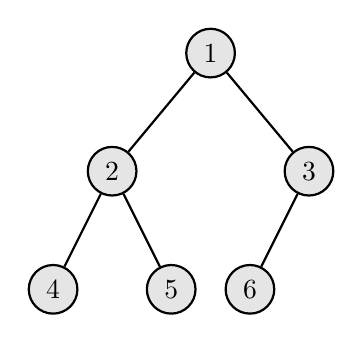
\begin{tikzpicture}
[every node/.style={draw, circle, fill=gray!20!, minimum size=5mm},
level 1/.style={sibling distance=25mm},
level 2/.style={sibling distance=15mm},
thick]
\node{1}
child{node{2} child{node{4}} child{node{5}}}
child{node{3} child{node{6}} child[missing]};
\end{tikzpicture}
\end{figure}

\textbf{Output}: 6
\end{flushleft}

\subsection{Binary Search}
In a complete binary tree every level, except possibly the last, is completely filled, and all nodes in the last level are as far left as possible.

Suppose the level of the tree is $d$ (level is from 0 to $d$). The number of nodes in all levels but the last one is $2^d - 1$. The number of nodes in the last level could vary from 1 to $2^d$.

Enumerate potential nodes from 0 to $2^d - 1$1 and perform the binary search by the node index to check how many nodes are in the last level.

\setcounter{lstlisting}{0}
\begin{lstlisting}[style=customc, caption={Binary Search}]
int countNodes( TreeNode* root )
{

    if( !root )
    {
        return 0;
    }
    //get the depth of tree
    //tree are from level 0 to level d
    auto d( get_depth( root ) );
    if( d == 0 )
    {
        return 1;
    }
    //find if a index in the last level exists
    int left = 0;
    int right = ( 1 << d ) - 1;
    while( left <= right )
    {
        auto mid( left + ( right - left ) / 2 );
        if( found( mid, d, root ) )
        {
            left = mid + 1;
        }
        else
        {
            right = mid - 1;
        }
    }
    //level 0 to level (d-1) we have 2^d-1 nodes
    //and (left) nodes at level (d)
    return ( 1 << d ) - 1 + left;
}
//helper function to get depth
int get_depth( TreeNode* node )
{
    int d = 0;
    while( node->left )
    {
        ++d;
        node = node->left;
    }
    return d;
}
//helper function to check if a node with (idx)
//exists at level d
bool found( int idx, int d, TreeNode* node )
{
    //at level d
    //index of each node is from 0
    //to (2^d-1) for complete binary tree
    int left = 0;
    int right = ( 1 << d ) - 1;
    for( int level = 0; level < d; ++level )
    {
        auto mid( left + ( right - left ) / 2 );
        if( idx <= mid )
        {
            //idx in left child tree
            //search range is [left, mid]
            right = mid;
            node = node->left;
        }
        else
        {
            //idx in right child tree
            //search range is [mid+1,right]
            left = mid + 1;
            node = node->right;
        }
    }
    return node;
}
\end{lstlisting}

\subsection{Iterative Approach}
We can find the leftmost and rightmost path from \fcj{root} to the leaf node. If the lengths of both are equal, the last level will have $2^d-1$ nodes (perfect binary tree). Otherwise, the number of nodes in the left and right subtree is the answer.

\begin{lstlisting}[style=customc, caption={Recursive}]
int countNodes( TreeNode* root )
{
    auto ltree = root;
    auto d_left( 0 );
    while( ltree )
    {
        ltree = ltree->left;
        ++d_left;
    }
    auto rtree = root;
    auto d_right( 0 );
    while( rtree )
    {
        rtree = rtree->right;
        ++d_right;
    }
    if( d_left == d_right )
    {
        //perfert complete binary tree
        return ( 1 << d_left ) - 1;
    }
    //otherwise return the left and right subtree nodes
    return countNodes( root->left ) + countNodes( root->right ) + 1;
}
\end{lstlisting}
%\section{223 --- Rectangle Area}
Find the total area covered by two rectilinear rectangles in a 2D plane.
\par
Each rectangle is defined by its bottom left corner and top right corner as shown in the figure.
\begin{figure}[H]
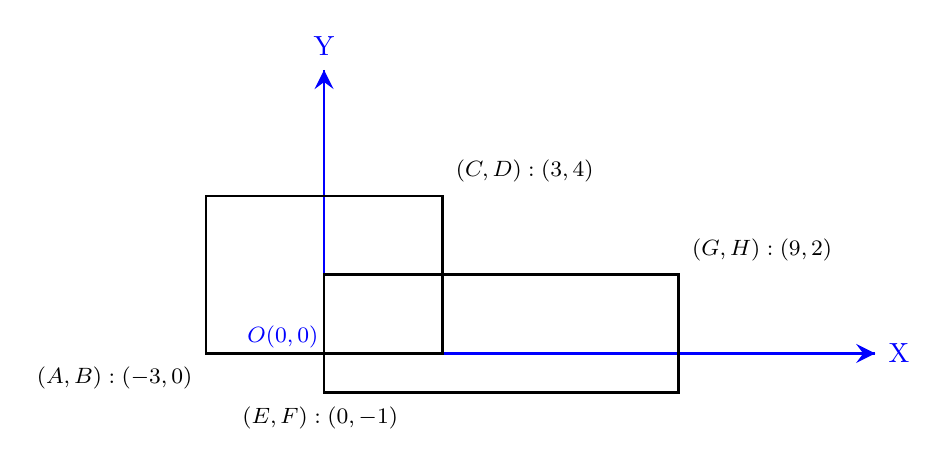
\begin{tikzpicture}
\draw[decoration={markings,mark=at position 1 with
    {\arrow[scale=1.5,>=stealth]{>}}},postaction={decorate}, line width=1pt, color=blue] (0,0) -- (7,0);
\draw[decoration={markings,mark=at position 1 with
    {\arrow[scale=1.5,>=stealth]{>}}},postaction={decorate}, line width=1pt, color=blue] (0,0) -- (0,3.6);
\node(0) at (7.3,0) {{\textcolor{blue}{X}}};
\node(1) at (0,3.9) {{\textcolor{blue}{Y}}};
\draw[line width=1pt] (-1.5,0) rectangle (1.5,2);
\draw[line width=1pt] (0,-0.5) rectangle (4.5,1);
\node() [anchor = south west] at (1.55,2.05) {\footnotesize $(C,D):(3,4)$};
\node() [anchor = north east] at (-1.55,-0.05) {\footnotesize $(A,B):(-3,0)$};
\node() [anchor = south east] at (0.05, -0.05) {\footnotesize \textcolor{blue}{$O(0,0)$}};
\node() [anchor = south west] at (4.55,1.05) {\footnotesize $(G,H):(9,2)$};
\node() [anchor = north] at (-0.05,-0.55) {\footnotesize $(E,F):(0,-1)$};
\end{tikzpicture}
\end{figure}

\paragraph{Example:}
\begin{flushleft}
\textbf{Input}: $A = -3$, $B = 0$, $C = 3$, $D = 4$, $E = 0$, $F = -1$, $G = 9$, $H = 2$
\\
\textbf{Output}: 45
\end{flushleft}

\paragraph{Note:}

\begin{itemize}
\item Assume that the total area is never beyond the maximum possible value of \texttt{int}.
\end{itemize}
\subsection{Geometry}
\begin{itemize}
\item 算出两个矩形的面积和
\item 确定两个矩形是否overlap,其实只有四种情形需要考虑,即 $B\geq H$ or $E\geq C$ or $F\geq D$ or $A\geq G$.
\item 如果overlapped,需要确定overlapped 部分的bottem left和top right。其中left为$\max(A,E)$, bottom为$\max(B, F)$。而top则等于$\min(C,G)$, right
等于$\min(D,H)$。
\item 为了避免出现数据精度overflow,所有的宽度和高度计算都转换成\texttt{long long}
\end{itemize}

\setcounter{lstlisting}{0}
\begin{lstlisting}[style=customc, caption={Geometry}]
int computeArea( int A, int B, int C, int D, int E, int F, int G, int H )
{
    long long w = C - A;
    long long h = D - B;
    auto ans = w * h;
    w = G - E;
    h = H - F;
    ans += w * h;

    if( ( A >= G ) || ( B >= H ) || ( E >= C ) || ( F >= D ) )
    {
        return ans;
    }
    w = ( min )( C, G ) - ( max )( A, E );
    h = ( min )( D, H ) - ( max )( B, F );
    return ans - w * h;
}
\end{lstlisting}
\section{224 --- Basic Calculator}
Implement a basic calculator to evaluate a simple expression string $S$.
\par
The expression string may contain open ( and closing parentheses ), the plus or minus sign, non-negative integers and empty spaces .

\paragraph{Example 1:}
\begin{flushleft}
\textbf{Input}: $1\ +\ 1$
\\
\textbf{Output}: 2
\end{flushleft}

\paragraph{Example 2:}
\begin{flushleft}
\textbf{Input}: $2-1\ +\ 2$
\\
\textbf{Output}: 3
\end{flushleft}

\paragraph{Example 3:}
\begin{flushleft}
\textbf{Input}: $(1+(4+5+2)-3)+(6+8)$
\\
\textbf{Output}: 23
\end{flushleft}

\paragraph{Note:}

\begin{itemize}
\item You may assume that the given expression is always valid.
\item Do not use the \texttt{eval} built-in library function.
\end{itemize}
\subsection{Stack}
\begin{itemize}
\item 由于只涉及到加法和减法,因此可以统一用加法来处理,遇到减号则将后面跟随的数字设置为负数即可。
\item 每次遇到左括号,就将之前得到的结果和符号标记分别压入对应的stack中。所以需要两个stack。
\item 每次遇到右括号,则分别将两个stack中顶端的数字加上符号与括号中的值相乘得到的结果即为当前表达式的值。
\item 如果表达式是以数字结束的,那么在最后仍然需要将获得的数字和符号进行相乘加到之前的表达式结果中。否则最后的操作符和数字就会忽略掉。
\end{itemize}

\setcounter{lstlisting}{0}
\begin{lstlisting}[style=customc, caption={Stack}]
int calculate( string s )
{
    stack<long long> stk_nums;
    stack<long long> stk_ops;

    long long num = 0;
    long long sign = 1;

    long long last = 0;

    for( auto c : s )
    {
        if( c >= '0' && c <= '9' )
        {
            num = num * 10 + ( c - '0' );
            continue;
        }


        last += num * sign;
        num = 0;

        switch( c )
        {
        case '+':
            sign = 1;
            break;
        case '-':
            sign = -1;
            break;

        case '(':
            stk_nums.push( last );
            stk_ops.push( sign );
            last = 0;
            sign = 1;
            break;

        case ')':
            last = stk_ops.top() * last + stk_nums.top();
            stk_ops.pop();
            stk_nums.pop();
            break;
        }
    }

	// When S is ended with number, need to 
	// compute the last one
    last += num * sign;

    return static_cast< int >( last );
}
\end{lstlisting}
%\section{225 --- Implement Stack using Queues}
Implement the following operations of a stack using queues.

\begin{itemize}
\item \texttt{push(x)} -- Push element x onto stack.
\item \texttt{pop()} -- Removes the element on top of the stack.
\item \texttt{top()} -- Get the top element.
\item \texttt{empty()} -- Return whether the stack is empty.
\end{itemize}
\paragraph{Example:}
\begin{lstlisting}[style=customc]
MyStack stack = new MyStack();

stack.push(1);
stack.push(2);  
stack.top();   // returns 2
stack.pop();   // returns 2
stack.empty(); // returns false
\end{lstlisting}

\paragraph{Notes:}

\begin{itemize}
\item You must use only standard operations of a queue -- which means only \texttt{push} to back,\texttt{ peek/pop} from front, \texttt{size}, and \texttt{is empty} operations are valid.
\item Depending on your language, queue may not be supported natively. You may simulate a queue by using a list or deque (double-ended queue), as long as you use only standard operations of a queue.
\item You may assume that all operations are valid (for example, no pop or top operations will be called on an empty stack).
\end{itemize}
\subsection{One queue}
\begin{CJK*}{UTF8}{gbsn}
这题一般的思路是用两个queue,然后当需要进行pop时,就将其中一个queue中的元素弹出放入另外一个queue。这无形中增加了memory的需求。其实这题可以借助一个queue来完成,即每次加入一个元素后,检查当前queue的size是否大于1。 如果大于1,则不停的将queue的front弹出重新加入queue中,直到处理到当前加入的元素。每次这样操作后,queue中的元素排列顺序就和stack是一样的了。
\end{CJK*}
\setcounter{lstlisting}{0}
\begin{lstlisting}[style=customc, caption={Queue}]
class MyStack
{
public:
    /** Initialize your data structure here. */
    MyStack()
    {
    }

    /** Push element x onto stack. */
    void push( int x )
    {
        q.push( x );

        auto sz = q.size();

		//make sure the loop stop at current element x
        while( sz > 1 )
        {
            int t = q.front();
            q.pop();
            q.push( t );

            --sz;
        }
    }

    /** Removes the element on top of the stack and returns that element. */
    int pop()
    {
        int t = q.front();
        q.pop();

        return t;
    }

    /** Get the top element. */
    int top()
    {
        return q.front();
    }

    /** Returns whether the stack is empty. */
    bool empty()
    {
        return q.empty();
    }

    queue<int> q;
};


\end{lstlisting}
%\section{226 --- Invert Binary Tree}
Invert a binary tree.

\paragraph{Example:}
\begin{flushleft}


\textbf{Input:}
\begin{figure}[H]
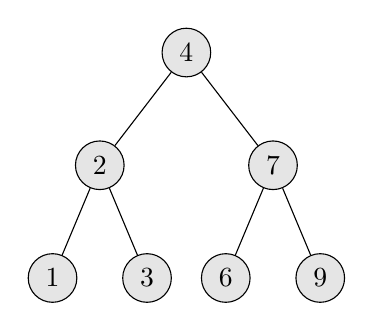
\begin{tikzpicture}
[mynode/.style={draw,circle,minimum size=5mm, fill=gray!20!}]
\node(){};
\node[mynode](1) {4};
\node[mynode](2)[below=8mm of 1, xshift=-11mm] {2};
\node[mynode](3)[below=8mm of 1, xshift=11mm] {7};
\node[mynode](4)[below=8mm of 2, xshift=-6mm] {1};
\node[mynode](5)[below=8mm of 2, xshift=6mm] {3};
\node[mynode](6)[below=8mm of 3, xshift=-6mm] {6};
\node[mynode](7)[below=8mm of 3, xshift=6mm] {9};
\draw (1) -- (2);
\draw (1) -- (3);
\draw (2) -- (4);
\draw (2) -- (5);
\draw (3) -- (6);
\draw (3) -- (7);
\end{tikzpicture}
\end{figure}
\textbf{Output:}
\begin{figure}[H]
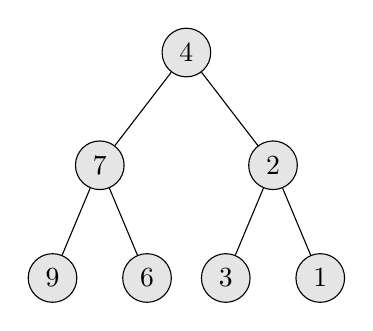
\begin{tikzpicture}
[mynode/.style={draw,circle,minimum size=5mm, fill=gray!20!}]
\node(){};
\node[mynode](1) {4};
\node[mynode](2)[below=8mm of 1, xshift=-11mm] {7};
\node[mynode](3)[below=8mm of 1, xshift=11mm] {2};
\node[mynode](4)[below=8mm of 2, xshift=-6mm] {9};
\node[mynode](5)[below=8mm of 2, xshift=6mm] {6};
\node[mynode](6)[below=8mm of 3, xshift=-6mm] {3};
\node[mynode](7)[below=8mm of 3, xshift=6mm] {1};
\draw (1) -- (2);
\draw (1) -- (3);
\draw (2) -- (4);
\draw (2) -- (5);
\draw (3) -- (6);
\draw (3) -- (7);
\end{tikzpicture}
\end{figure}
\end{flushleft}
\subsection{Recursion}

对于每一个节点,都是相同的操作,
\begin{itemize}
\item 获得当前节点的左右子节点
\item 分别对左右子节点进行\textbf{invert}操作
\item 将当前节点的左子节点指向invert后的右子树
\item 将当前节点的右子节点指向invert后的左子数。
\end{itemize}
\setcounter{lstlisting}{0}
\begin{lstlisting}[style=customc, caption={Recursion}]
TreeNode* invertTree( TreeNode* root )
{

    if( !root )
    {
        return root;
    }

    auto l = root->left;
    auto r = root->right;

    root->right = invertTree( l );
    root->left = invertTree( r );

    return root;
}
\end{lstlisting}
%\section{227 --- Basic Calculator II}
Implement a basic calculator to evaluate a simple expression string $S$.
\par
The expression string contains only non-negative integers, $+$, $-$, $\times$, $\div$ operators and empty spaces . The integer division should truncate toward zero.

\paragraph{Example 1:}

\begin{flushleft}
\textbf{Input}: $3+2\times2$
\\
\textbf{Output}: 7
\end{flushleft}

\paragraph{Example 2:}

\begin{flushleft}
\textbf{Input}: $ 3\div2 $
\\
\textbf{Output}: 1
\end{flushleft}

\paragraph{Example 3:}

\begin{flushleft}
\textbf{Input}:  $3+5\div2$
\\
\textbf{Output}: 5
\end{flushleft}

\paragraph{Note:}

\begin{itemize}
\item You may assume that the given expression is always valid.
\item Do not use the \texttt{eval} built-in library function.
\end{itemize}

\subsection{Two Stacks}
\begin{CJK*}{UTF8}{gbsn}
\begin{itemize}
\item 用两个stack,一个放数字 $S_1$,一个放操作符 $S_2$。其中$S_2$只放入除法或者乘法。
\item 与224类似,用一个sign来表示正负数,这样就避免了进行减法的操作。
\item 由于没有括号,所以相对来说比较容易处理,如果$S_2$不为空,则将$S_1$的栈顶元素弹出,和当前获得的number进行除法或者乘法操作,然后再加入$S_1$中。
\item 遍历$S$结束后,由于最后一个数字和操作符没有被处理,仍然需要先处理。
\item 最后,陆续弹出$S_1$中的元素,将它们相加即为所求结果。
\end{itemize}
\end{CJK*}

\setcounter{algorithm}{0}
\begin{algorithm}[H]
\caption{Two Stacks}
\begin{algorithmic}[1]
\Procedure{Calculate}{$S$}
\State $\star$ Prepare two stacks $S_1$ and $S_2$
\State $n:=0$ \Comment The current number
\State $z:=1$ \Comment The sign
\For{Each character $c$ in $S$}
\If{$c$ is a space}
\State \texttt{Continue} \Comment Skip space
\EndIf
\If{$c$ is a digit}
\State $n\gets n\times 10 + \texttt{Int}(c)$ \Comment Update $n$
\State \texttt{Continue}
\EndIf
\State $n\gets n\times z$ \Comment Update $n$ by the sign
\If{$S_2$ is not empty} \Comment We have met $\times$ or $\div$ before
\State $\star$ Get and pop top of $S_1$ as $t_1$
\State $\star$ Get and pop top of $S_2$ as \texttt{op}
\State $\star$ Push the result of $t_1$ \texttt{op} $n$ to $S_1$
\Else
\State $\star$ Push $n$ to $S_1$ \Comment No $\times$ or $\div$ was found before
\EndIf
\If{$c$ is $\times$ or $\div$}
\State $z\gets 1$ \Comment Reset sign to 1
\State $\star$ Push $c$ to $S_2$
\ElsIf{$c$ is $+$}
\State $z\gets 1$ \Comment Reset sign to 1
\ElsIf{$c$ is $-$}
\State $z\gets -1$ \Comment Reset sign to $-1$
\EndIf
\EndFor
\State $n\gets n\times z$ \Comment $n$ is the last number that has not been processed
\State $\ast$ We still need to check if the last operation is $\times$ or $\div$ after the iteration over $S$ is completed
\algstore{227algo}
\end{algorithmic}
\end{algorithm}
\begin{algorithm}[H]
\begin{algorithmic}[1]
\algrestore{227algo}
\If{$S_2$ is not empty} \Comment We have met $\times$ or $\div$ before
\State $\star$ Get and pop top of $S_1$ as $t_1$
\State $\star$ Get and pop top of $S_2$ as \texttt{op}
\State $\star$ Push the result of $t_1$ \texttt{op} $n$ to $S_1$
\Else
\State $\star$ Push $n$ to $S_1$ \Comment No $\times$ or $\div$ was found before
\EndIf
\State $\ast$ Add all numbers in $S_1$ to get the final result
\State $\sigma:=0$ \Comment The total sum
\While{$S_1$ is not empty}
\State $\star$ Add top of $S_1$ to $\sigma$
\State $\star$ Pop top of $S_1$
\EndWhile
\State \Return $\sigma$
\EndProcedure
\end{algorithmic}
\end{algorithm}
\setcounter{lstlisting}{0}
\begin{lstlisting}[style=customc, caption={Two Stacks}]
int calculate( string s )
{

    stack<long long> stk;
    stack<char> ops;

    long long num = 0;
    long long sign = 1;

    long long last = 0;
    for( auto c : s )
    {
        if( c == ' ' )
        {
            continue;
        }

        if( c >= '0' && c <= '9' )
        {
            num = num * 10 + ( c - '0' );
            continue;
        }



        num *= sign;

        if( !ops.empty() )
        {
            auto t = stk.top();
            stk.pop();

            auto op = ops.top();
            ops.pop();

            switch( op )
            {
            case '*':
                stk.push( num * t );
                break;

            case '/':
                stk.push( t / num );
                break;
            }
        }
        else
        {
            stk.push( num );
        }

        num = 0;


        switch( c )
        {
        case '*':
        case '/':
            sign = 1;
            ops.push( c );
            break;

        case '+':
            sign = 1;
            break;

        case '-':
            sign = -1;
            break;
        }
    }

    num *= sign;
    if( !ops.empty() )
    {
        auto t = stk.top();
        stk.pop();

        auto op = ops.top();
        ops.pop();

        switch( op )
        {
        case '*':
            stk.push( num * t );
            break;

        case '/':
            stk.push( t / num );
            break;
        }
    }
    else
    {
        stk.push( num );
    }

    long long ans = 0;

    while( !stk.empty() )
    {
        ans += stk.top();
        stk.pop();
    }

    return static_cast< int >( ans );
}
\end{lstlisting}
%\section{228 --- Summary Ranges}
Given a sorted integer array $A$ without duplicates, return the summary of its ranges.

\paragraph{Example 1:}

\begin{flushleft}
\textbf{Input}:  $[0,1,2,4,5,7]$
\\
\textbf{Output}: $[0\to2, 4\to5, 7]$
\\
\textbf{Explanation}: $0,1,2$ form a continuous range; $4,5$ form a continuous range.
\end{flushleft}

\paragraph{Example 2:}

\begin{flushleft}
\textbf{Input}:  $[0,2,3,4,6,8,9]$
\\
\textbf{Output}: $[0,2\to4,6,8\to9]$
\\
\textbf{Explanation}: $2,3,4$ form a continuous range; $8,9$ form a continuous range.
\end{flushleft}
\subsection{Plain Algorithm}
\begin{CJK*}{UTF8}{gbsn}
\begin{itemize}
\item 遍历数组,然后寻找连续数的segment。
\item 需要小心处理每一个分割点。
\item 需要将\texttt{int} type升级成\texttt{long long} type以处理数据精度overflow。
\end{itemize}
\end{CJK*}
\setcounter{lstlisting}{0}
\begin{lstlisting}[style=customc, caption={Plain Algorithm}]
vector<string> summaryRanges( vector<int>& nums )
{

    if( nums.empty() )
    {
        return {};
    }

    vector<string> ans;

    // Need to check if the back of nums has been
    // added into a range
    int last_end = nums.back() + 1;

    long long a = 0;
    long long b = 0;

    for( size_t i = 0; i < nums.size() - 1; ++i )
    {
        a = static_cast<long long>( nums[i + 1] );
        b = static_cast<long long>( nums[i] );
        if( a - b == 1 )
        {
            size_t j = i + 1;

            while( j < nums.size() - 1 )
            {
                a = static_cast<long long>( nums[j + 1] );
                b = static_cast<long long>( nums[j] );

                if( a - b != 1 )
                {
                    break;
                }
                ++j;
            }

            string s = to_string( nums[i] );
            s += "->";
            s += to_string( nums[j] );

            ans.emplace_back( s );
            i = j;

            //update range end
            last_end = nums[j];
        }
        else
        {
            ans.emplace_back( to_string( nums[i] ) );
            //update range end
            last_end = nums[i];
        }
    }

    if( nums.back() != last_end )
    {
        ans.emplace_back( to_string( nums.back() ) );
    }
    return ans;
}
\end{lstlisting}
%\section{229 --- Majority Element II}
Given an integer array $A$ of size $n$, find all elements that appear more than $\lfloor n/3 \rfloor$ times.
\par
Note: The algorithm should run in linear time and in O(1) space.

\paragraph{Example 1:}

\begin{flushleft}
\textbf{Input}: $[3,2,3]$
\\
\textbf{Output}: $[3]$
\end{flushleft}

\paragraph{Example 2:}

\begin{flushleft}
\textbf{Input}: $[1,1,1,3,3,2,2,2]$
\\
\textbf{Output}: $[1,2]$
\end{flushleft}
\subsection{Boyer-Moore Voting Algorithm}
In the first pass, we generate a single candidate value which is the majority value if there is a majority. The second pass simply counts the frequency of that value to confirm. The first pass is the interesting part.
\par
In the first pass, we need 2 values:
\begin{itemize}
\item A candidate value, initially set to any value.
\item A count, initially set to 0.
\end{itemize}
For each element in our input list, we first examine the count value. If the count is equal to 0, we set the candidate to the value at the current element. Next, first compare the element's value to the current candidate value. If they are the same, we increment count by 1. If they are different, we decrement count by 1.
\par
At the end of all of the inputs, the candidate will be the majority value if a majority value exists. A second O(N) pass can verify that the candidate is the majority element.
\subsection{Two Candidates}
\begin{CJK*}{UTF8}{gbsn}
\begin{itemize}
\item 仍然是基于上述的Boyer-Moore Voting算法。
\item 由于这时候的candidates至多是两个(因为出现次数要大于$L/3$),所以需要两个counter。
\item 遍历$A$时,条件判断的顺序非常重要。必须先判定candidate是否和当前的数相等,再判断counter是否为零。如果顺序颠倒,那么当其中一个counter变为零时,会将当前数设置为对应的candidate,有可能和另一个candidate重复。比如$[1, 2, 2, 3, 2, 1, 1, 3]$
\end{itemize}
\end{CJK*}
\setcounter{algorithm}{0}
\begin{algorithm}[H]
\caption{Two Candidate Voting Algorithm}
\begin{algorithmic}[1]
\Procedure{MajorityElement}{$A, L$}
\State $\star$ Initialize two counters $\alpha$, $\beta$ as zeros
\State $\star$ Initialize two candidates $x$, $y$ as any value.
\For{Each number $n$ in $A$}
\State $\star$ The following sequence of condition checking cannot be changed
\If{$n=x$}
\State $\alpha\gets\alpha+1$ \Comment Increments counter associated with $x$
\ElsIf{$n=y$}
\State $\beta\gets\beta+1$ \Comment Increments counter associated with $y$
\ElsIf{$\alpha=0$}
\State $x\gets n$ \Comment Update candidate $x$
\State $\alpha\gets 1$
\ElsIf{$\beta=0$}
\State $y\gets n$ \Comment Update candidate $y$
\State $\beta\gets1$
\Else
\State $\alpha\gets\alpha-1$ \Comment Decrements counter associated with $x$
\State $\beta\gets\beta-1$ \Comment Decrements counter associated with $y$
\EndIf
\EndFor
\State $\ast$ Check if $x$ and $y$ are actually the major elements
\State $\alpha\gets 0$
\State $\beta\gets 0$
\For{Each number $n$ in $A$}
\If{$n=x$}
\State $\alpha\gets\alpha+1$
\ElsIf{$n=y$}
\State $\beta\gets\beta+1$
\algstore{229algo}
\end{algorithmic}
\end{algorithm}
\begin{algorithm}[H]
\begin{algorithmic}[1]
\algrestore{229algo}
\EndIf
\EndFor
\If{$\alpha > L/3$}
\State $\star$ Add $x$ to the final list 
\EndIf
\If{$\beta > L/3$}
\State $\star$ Add $y$ to the final list
\EndIf
\State $\star$ Return the final list
\EndProcedure
\end{algorithmic}
\end{algorithm}
\setcounter{lstlisting}{0}
\begin{lstlisting}[style=customc, caption={Two Candidates Voting Algorithm}]
vector<int> majorityElement( vector<int>& nums )
{
    int n1 = 0;
    int n2 = 0;
    int count1 = 0;
    int count2 = 0;

    // The following condition checking sequence
    // cannot be changd.
    for( auto n : nums )
    {
        if( n1 == n )
        {
            ++count1;
        }
        else if( n2 == n )
        {
            ++count2;
        }
        else if( count1 == 0 )
        {
            n1 = n;
            ++count1;
        }
        else if( count2 == 0 )
        {
            n2 = n;
            ++count2;
        }
        else if( n2 == n )
        {
            ++count2;
        }
        else
        {
            --count1;
            --count2;
        }
    }

    count1 = 0;
    count2 = 0;

    for( auto n : nums )
    {
        if( n == n1 )
        {
            ++count1;
        }
        else if( n == n2 )
        {
            ++count2;
        }
    }

    //The threshold for major elements
    int th = static_cast<int>( nums.size() ) / 3;

    vector<int> ans;

    if( count1 > th )
    {
        ans.push_back( n1 );
    }

    if( count2 > th )
    {
        ans.push_back( n2 );
    }

    return ans;
}
\end{lstlisting}
%\section{230 --- Kth Smallest Element in a BST}
Given a binary search tree, write a function to find the $k$th smallest element in it.
\par
\paragraph{Note: }
\begin{itemize}
\item You may assume $k$ is always valid, $1 \leq k \leq$ BST's total elements.
\end{itemize}

\paragraph{Example 1:}
\begin{flushleft}

\textbf{Input}: 
\begin{figure}[H]
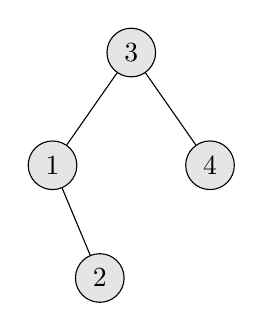
\begin{tikzpicture}
[mynode/.style={draw,circle,minimum size=5mm, fill=gray!20!}]
\node(){};
\node[mynode](1) {3};
\node[mynode](2)[below=8mm of 1, xshift=-10mm] {1};
\node[mynode](3)[below=8mm of 1, xshift=10mm] {4};
\node[mynode](4)[below=8mm of 2, xshift=6mm] {2};
\draw (1)--(2);
\draw (1)--(3);
\draw (2)--(4);
\end{tikzpicture}
\end{figure}
$k = 1$
\\
\textbf{Output}: 1
\end{flushleft}

\paragraph{Example 2:}

\begin{flushleft}
Input:
\begin{figure}[H]
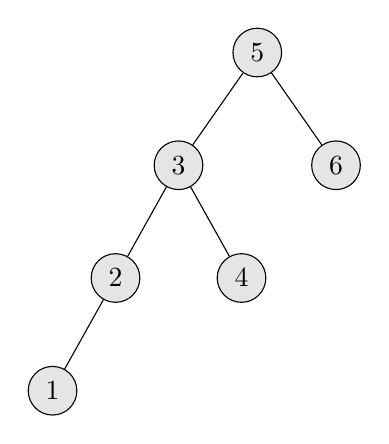
\begin{tikzpicture}
[mynode/.style={draw,circle,minimum size=5mm, fill=gray!20!}]
\node(){};
\node[mynode](1) {5};
\node[mynode](2)[below=8mm of 1, xshift=-10mm] {3};
\node[mynode](3)[below=8mm of 1, xshift=10mm] {6};
\node[mynode](4)[below=8mm of 2, xshift=-8mm] {2};
\node[mynode](5)[below=8mm of 2, xshift=8mm] {4};
\node[mynode](6)[below=8mm of 4, xshift=-8mm] {1};
\draw (1)--(2);
\draw (1)--(3);
\draw (2)--(4);
\draw (2)--(5);
\draw (4)--(6);
\end{tikzpicture}
\end{figure}
$k = 3$
\par
\textbf{Output}: 3
\end{flushleft}

\paragraph{Follow up:}
\begin{itemize}
\item What if the BST is modified (insert/delete operations) often and you need to find the $k$th smallest frequently? How would you optimize the function?
\end{itemize}
\subsection{In-order Traverse}
\begin{CJK*}{UTF8}{gbsn}
\begin{itemize}
\item 仔细分析就可以看出,由于BST的特性,中序遍历其实就是从小到大的顺序。
\item 因此求$k$th smallest element就变成中序遍历中记录当前访问元素是否是遍历到的第$k$个数字即可。
\item 中序遍历可以使用stack,递归,以及Morris Traverse。
\end{itemize}
\end{CJK*}
\setcounter{lstlisting}{0}
\begin{lstlisting}[style=customc, caption={Stack Based In-order Traverse}]
int kthSmallest( TreeNode* root, int k )
{
    int cnt = 0;
    stack<TreeNode*> s;
    TreeNode *p = root;
    while( p || !s.empty() )
    {
        while( p )
        {
            s.push( p );
            p = p->left;
        }
        p = s.top();
        s.pop();
        ++cnt;
        if( cnt == k ) return p->val;
        p = p->right;
    }
    return 0;
}
\end{lstlisting}
\begin{lstlisting}[style=customc, caption={Recursion Based In-order Traverse}]
int kthSmallest( TreeNode* root, int k )
{

    int x = 0;
    int val = -1;

    inorder( root, k, x, val );

    return val;

}
//x is the count of current node when traversing the tree
//val is the visited kth number when traversing the tree
void inorder( TreeNode* node, int k, int& x, int& val )
{
    if( !node )
    {
        return;
    }

    inorder( node->left, k, x, val );

    ++x;

    if( x == k )
    {
        val = node->val;
        return;
    }

    inorder( node->right, k, x, val );
}
\end{lstlisting}
\subsection{Divide And Conquer}
\begin{CJK*}{UTF8}{gbsn}
\begin{itemize}
\item 由于BST的性质,可以快速定位出第$k$小的元素是在左子树还是右子树,
\item 首先计算出左子树的结点个数总和$t$,
\item 如果$k\leq t$,说明第k小的元素在左子树中,直接对左子结点调用递归即可。
\item 如果$k>t+1$,说明目标值在右子树中,对右子结点调用递归函数,注意此时的$k$需要更新为$k-t-1$,因为已经减少了左子树和根节点总计$t+1$个结点。
\item 如果$k=t+1$,说明当前结点即为所求,返回当前结点值即可
\end{itemize}
\end{CJK*}
\begin{lstlisting}[style=customc, caption={Divide And Conquer}]
int kthSmallest( TreeNode* root, int k )
{
    int count = countNodes( root->left );

    if( k <= count )
    {
        return kthSmallest( root->left, k );
    }
    else if( k > count + 1 )
    {
        return kthSmallest( root->right, k - count - 1 );
    }

    return root->val;
}

int countNodes( TreeNode* root )
{
    if( !root )
    {
        return 0;
    }

    return 1 + countNodes( root->left ) + countNodes( root->right );
}
\end{lstlisting}
\subsection{Follow Up}
\begin{CJK*}{UTF8}{gbsn}
\begin{itemize}
\item 如果该BST被修改的很频繁,而且查找操作也很频繁,那么最好的方法还是用分治法来快速定位目标所在的位置,
\item 分治法中最低效的部分在于每次都需要遍历左子树所有结点来计算个数。
\item 为了提升效率,需要修改\texttt{TreeNode struct},在其中保存包括当前结点和其左右子树所有结点的个数,这样就可以快速得到任何左子树结点总数。
\item 由于\texttt{TreeNode struct}被修改了,因此需要重新build BST。然后再进行查找$k$th smallest element的操作。
\end{itemize}
\end{CJK*}
\begin{lstlisting}[style=customc, caption={Follow Up}]
class Solution
{
public:

    // New struct
    struct CountNode
    {
        int val;
        int counts;

        CountNode *left;
        CountNode *right;

        CountNode( int x )
            : val( x )
            , counts( 1 )
            , left( nullptr )
            , right( nullptr )
        {}
    };

    CountNode* build( TreeNode* root )
    {
        if( !root )
        {
            return nullptr;
        }
        // node->counts is set to 1 when constructed
        CountNode* node = new CountNode( root->val );
        node->left = build( root->left );
        node->right = build( root->right );

        //Update current node's node counts.
        if( node->left )
        {
            node->counts += node->left->counts;
        }

        if( node->right )
        {
            node->counts += node->right->counts;
        }


        return node;
    }

    int searchKthSmallest( CountNode* root, int k )
    {
        if( root->left )
        {
            //The target is in left subtree
            if( k <= root->left->counts )
            {
                return searchKthSmallest( root->left, k );
            }

            //The target is in right subtree
            if( k > root->left->counts + 1 )
            {
                return searchKthSmallest( root->right, k - root->left->counts - 1 );
            }

            return root->val;
        }
        else
        {
            //since left subtree is empty
            //Then we can assume root->left->counts=0
            if( k > 1 )
            {
                return searchKthSmallest( root->right, k - 1 );
            }

            return root->val;
        }
    }

    int kthSmallest( TreeNode* root, int k )
    {

        //build new tree based on CountNode struct
        CountNode* node = build( root );

        return searchKthSmallest( node, k );
    }
};
\end{lstlisting}
%\section{231 --- Power of Two}
Given an integer $n$, write a function to determine if it is a power of two.

\paragraph{Example 1:}

\begin{flushleft}
\textbf{Input}: 1
\\
\textbf{Output}: \texttt{true} 
\\
\textbf{Explanation}: $2^0 = 1$
\end{flushleft}


\paragraph{Example 2:}

\begin{flushleft}
\textbf{Input}: 16
\\
\textbf{Output}: \texttt{true}
\\
\textbf{Explanation}: $2^4 = 16$
\end{flushleft}

\paragraph{Example 3:}
\begin{flushleft}
\textbf{Input}: 218
\\
\textbf{Output}: \texttt{false}
\end{flushleft}
\subsection{Bit Operation}

\begin{itemize}
\item 利用$n$\&$(n-1)$能够消除rightmost 1-bit的特性。如果是2的power,那么$n$\&$(n-1)$就为零。
\item 需要考虑当$n$是int type所能代表的最大和最小值,以及$n=0$。这三种情况都返回\texttt{false}。
\end{itemize}

\setcounter{lstlisting}{0}
\begin{lstlisting}[style=customc, caption={Bit Operation}]
bool isPowerOfTwo( int n )
{
    if( n == INT_MAX || n == INT_MIN || n == 0 )
    {
        return false;
    }

    int x = ( ( n - 1 ) & n );

    return x == 0;
}
\end{lstlisting}
%\section{232 --- Implement Queue using Stacks}
Implement the following operations of a queue using stacks.
\begin{flushleft}
\begin{lstlisting}[style=customc]
push(x) //Push element x to the back of queue.
pop() //Removes the element from in front of queue.
peek() //Get the front element.
empty() //Return whether the queue is empty.
\end{lstlisting}
\end{flushleft}

\paragraph{Example:}

\begin{flushleft}
\begin{lstlisting}[style=customc]
MyQueue queue = new MyQueue();

queue.push(1);
queue.push(2);  
queue.peek();  // returns 1
queue.pop();   // returns 1
queue.empty(); // returns false
\end{lstlisting}
\end{flushleft}

\paragraph{Notes:}

\begin{itemize}
\item You must use only standard operations of a stack -- which means only \texttt{push} to \texttt{top}, \texttt{peek}/\texttt{pop} from top, \texttt{size}, and \texttt{is empty} operations are valid.
\item Depending on your language, stack may not be supported natively. You may simulate a stack by using a list or deque (double-ended queue), as long as you use only standard operations of a stack.
\item You may assume that all operations are valid (for example, no \texttt{pop} or \texttt{peek} operations will be called on an empty queue).
\end{itemize}
\subsection{Two Stacks}
\begin{CJK*}{UTF8}{gbsn}
\begin{itemize}
\item 因为是queue,所以新加入的number需要push到bottom of the stack.
\begin{enumerate}
\item 首先把$S_1$中的所有number都转移到辅助栈$S_2中$
\item 然后把新加入的number push到$S_2$中,这时候这个新的number就在$S_2$中的top上。
\item 再将$S_2$中的所有元素弹出,push到$S_1$。
\end{enumerate}
\item 由于上述push的操作,$S_1$总是把第一个插入的number放在top。因此直接从$S_1$弹出top即可。
\item 这种方法中,$S_2$只是用于reverse input numbers的顺序,因此除了push函数中会暂时有numbers进入,其余任何时候都是empty。
\end{itemize}
\end{CJK*}
\setcounter{lstlisting}{0}
\begin{lstlisting}[style=customc,caption={Two Stacks}]
class MyQueue
{
public:
    /** Initialize your data structure here. */
    MyQueue()
    {
    }

    /** Push element x to the back of queue. */
    void push( int x )
    {
        if( stk1.empty() )
        {
            stk1.push( x );
            return;
        }

        //Pop all numbers in stk1 and push to stk2
        while( !stk1.empty() )
        {
            auto t = stk1.top();
            stk1.pop();

            stk2.push( t );
        }

        stk2.push( x );

        while( !stk2.empty() )
        {
            auto t = stk2.top();
            stk2.pop();

            stk1.push( t );
        }
    }

    /** Removes the element from in front of queue and returns that element. */
    int pop()
    {
        int t = stk1.top();
        stk1.pop();

        return t;
    }

    /** Get the front element. */
    int peek()
    {
        return stk1.top();
    }

    /** Returns whether the queue is empty. */
    bool empty()
    {
        return stk1.empty();
    }

    stack<int> stk1;
    stack<int> stk2;

    int front;
};
\end{lstlisting}
\subsection{Two Stacks With Amortized O(1)}
\begin{CJK*}{UTF8}{gbsn}
\begin{itemize}
\item 新加入的number $x$总是放在$S_1$的top
\item 对于pop
\begin{enumerate}
\item 由于需要remove的number是位于$S_1$的底部,因此需要 pop all elements from $S_1$, 然后 push to $S_2$. 通过这种操作,$S_1$底部的number就成为$S_2$的top。
\item 只有当$S_2$为empty时,才进行上述操作,否则直接从$S_2$ pop。这就意味着在某些时刻,$S_1$和$S_2$同时都有多于1个的number。
\end{enumerate}
\item 这种方法中$S_2$和$S_1$有可能同时不为empty,因此取出queue的front元素就不能用方法1中直接从$S_1$中获得了,需要用一个辅助变量记录第一个插入的number。这样当$S_2$不为空时,表示此时还没有进行push操作,或者已经pop掉所有以前的numbers。
\end{itemize}
\setcounter{lstlisting}{0}
\begin{lstlisting}[style=customc, caption={Two Stack With Amortized O(1)}]
class MyQueue
{
public:
    /** Initialize your data structure here. */
    MyQueue()
    {
    }

    /** Push element x to the back of queue. */
    void push( int x )
    {
        //front is the first element of the queue
        //Need to set when the first time to call push()
        if( S1.empty() )
        {
            front = x;
        }

        S1.push( x );
    }

    /** Removes the element from in front of queue and returns that element. */
    int pop()
    {
        if( S2.empty() )
        {
            while( !S1.empty() )
            {
                auto t = S1.top();
                S1.pop();
                S2.push( t );
            }
        }

        auto t = S2.top();
        S2.pop();

        return t;
    }

    /** Get the front element. */
    int peek()
    {
        //Since S2 may contain input-reversed numbers
        //Need to check if S2 is empty or not
        //If it is not empty, the front element is S2's top
        //Otherwise, means push() has not been called
        //Or Pop() has been called to pop all numbers
        //Therefore, front variable is the current front
        if( !S2.empty() )
        {
            return S2.top();
        }
        else
        {
            return front;
        }
    }

    /** Returns whether the queue is empty. */
    bool empty()
    {
        return ( S1.empty() ) && ( S2.empty() );
    }

    stack<int> S1;
    stack<int> S2;

    int front;
};
\end{lstlisting}
\end{CJK*}
%\section{233 --- Number of Digit One}
Given an integer $n$, count the total number of digit 1 appearing in all non-negative integers less than or equal to $n$.

\paragraph{Example:}

\begin{flushleft}
\textbf{Input}: 13
\\
\textbf{Output}: 6 
\\
\textbf{Explanation}: 
\\
Digit 1 occurred in the following numbers: 1, 10, 11, 12, 13.
\end{flushleft}
\subsection{Solve it mathematically}
逐个分析个位,十位,百位。。。每个位上的1。

\begin{itemize}
\item 对于每一位,将$n$按照当前位分成两个部分。
\item 例如$n=3141592$,当分析百位上的1时,将$n$从百位上分成$a=31415$和$b=92$两个部分。因此从100到3141199,那么百位上的1出现的次数即为$3142\times 100$。乘以100是因为这是百位1,所以每次递增个位和十位时,百位上的1就重复了100次。而这个次数用$a$代表即为$(\lfloor a/10\rfloor+1)\times 100$。
\item 分析千位上的1时,$a=3141$而$b=592$。这时候如果仅仅考虑从1000到3141999,这个位上的1的出现次数为$315\times 1000$。但是$n=3141592 < 3141999$,因此千位上的1在百位,十位和个位递增时,只重复了593次,即从$1000$到$1592$。因此实际的重复次数是$314\times 1000 + 592$,用$a$和$b$表示即为 $(\lfloor a / 10\rfloor \times 1000) + (b + 1)$ times.
\item 上述情况的区分点在于要分析的位上的数字是否大于等于2,如果大于等于2,那么从$100\ldots0$到$199\ldots9$都能包括。否则就要考虑实际的重复次数了。
\end{itemize}

\setcounter{lstlisting}{0}
\begin{lstlisting}[style=customc, caption={Mathematical Induction}]
int countDigitOne( int n )
{
    long long a = 0;
    long long b = 0;

    auto lln = static_cast<long long>( n );

    long long ans = 0;

    for( long long p = 1; p <= lln; p *= 10 )
    {
        a = n / p;
        b = n - p * a;

        //check if the number at position p
        //which is r
        //is no less than 2 or not
        auto t = a / 10;
        auto r = a - 10 * t;

        if( r < 2 )
        {
            ans += t * p;
            ans += ( r == 1 ) ? ( b + 1 ) : 0; // need to count to 1(b)
        }
        else
        {
            ans += ( t + 1 ) * p; //Count from 10...0 to (t)19...9
        }
    }

    return static_cast<int>( ans );
}
\end{lstlisting}
%\section{234 --- Palindrome Linked List}
Given a singly linked list, determine if it is a palindrome.

\paragraph{Example 1:}

\begin{flushleft}
\textbf{Input}: 
\begin{figure}[H]
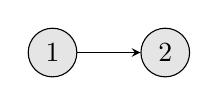
\begin{tikzpicture}
[mynode/.style={draw,circle,minimum size=5mm, fill=gray!20!}]
\node(){};
\node[mynode](1) {1};
\node[mynode](2)[right=8mm of 1] {2};
\draw[>=stealth,->] (1) -- (2);
\end{tikzpicture}
\end{figure}
\textbf{Output}: \texttt{false}
\end{flushleft}

\paragraph{Example 2:}

\begin{flushleft}
\textbf{Input}:
\begin{figure}[H]
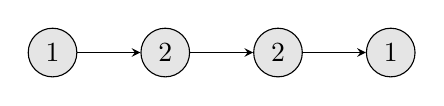
\begin{tikzpicture}
[mynode/.style={draw,circle,minimum size=5mm, fill=gray!20!}]
\node(){};
\node[mynode](1) {1};
\node[mynode](2)[right=8mm of 1] {2};
\node[mynode](3)[right=8mm of 2] {2};
\node[mynode](4)[right=8mm of 3] {1};
\draw[>=stealth,->] (1) -- (2);
\draw[>=stealth,->] (2) -- (3);
\draw[>=stealth,->] (3) -- (4);
\end{tikzpicture}
\end{figure}
\textbf{Output}: \texttt{true}
\end{flushleft}

\paragraph{Follow up:}
\begin{itemize}
\item Could you do it in $O(n)$ time and $O(1)$ space?
\end{itemize}
\subsection{Fast Slow Pointer And Reverse}

\begin{itemize}
\item 先用快慢指针找到链表的中间位置
\item 将中间位置往右的部分reverse
\item 比较前半部分链表和reverse的后半部分。
\end{itemize}


\setcounter{lstlisting}{0}
\begin{lstlisting}[style=customc, caption={Find Middle Reverse Right Half}]
bool isPalindrome( ListNode* head )
{

    if( !head || !head->next )
    {
        return true;
    }

    auto fast = head;
    auto slow = head;

    //find the middle of the linked list
    while( fast->next && fast->next->next )
    {
        slow = slow->next;
        fast = fast->next->next;
    }

    //Save the right half list head
    auto next_head = slow->next;
    //Break the list into left and right halves
    slow->next = nullptr;

    //Reverse the right half list
    ListNode* prev = nullptr;
    auto t = next_head;

    //Compare two halves
    while( t )
    {
        auto next = t->next;
        t->next = prev;
        prev = t;
        t = next;
    }

    auto n1 = head;
    //Now prev is the head of reversed right half list
    auto n2 = prev;

    while( n1 && n2 )
    {
        if( n1->val != n2->val )
        {
            return false;
        }

        n1 = n1->next;
        n2 = n2->next;
    }

    //Since we break at the middle of the linked list
    //Either the length of both halves are equal (even nodes)
    //or the left half has one more node than right half
    //(odd nodes)
    return true;
}
\end{lstlisting}
%\section{235 --- Lowest Common Ancestor of a Binary Search Tree}
Given a binary search tree (\texttt{BST}), find the lowest common ancestor (\texttt{LCA}) of two given nodes in the \texttt{BST}.
\par
According to the definition of \texttt{LCA} on \textbf{Wikipedia}: \textit{The lowest common ancestor is defined between two nodes $p$ and $q$ as the lowest node in $T$ that has both $p$ and $q$ as descendants (where we allow \textbf{a node to be a descendant of itself}).}

\paragraph{Example 1:}

\begin{flushleft}
\textbf{Input}: 
\begin{figure}[H]
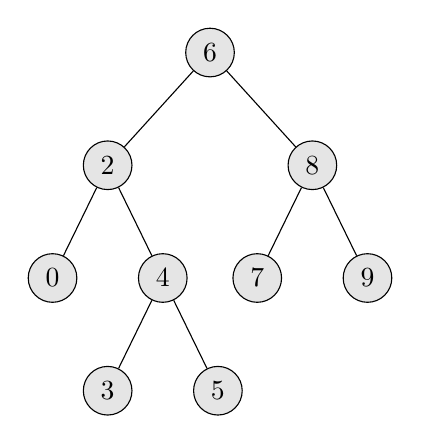
\begin{tikzpicture}
[mynode/.style={draw,circle,minimum size=5mm, fill=gray!20!}]
\node(){};
\node[mynode](1) {6};
\node[mynode](2)[below=8mm of 1, xshift=-13mm] {2};
\node[mynode](3)[below=8mm of 1, xshift=13mm] {8};
\node[mynode](4)[below=8mm of 2, xshift=-7mm] {0};
\node[mynode](5)[below=8mm of 2, xshift=7mm] {4};
\node[mynode](6)[below=8mm of 3, xshift=-7mm] {7};
\node[mynode](7)[below=8mm of 3, xshift=7mm] {9};
\node[mynode](8)[below=8mm of 5, xshift=-7mm] {3};
\node[mynode](9)[below=8mm of 5, xshift=7mm] {5};
\draw (1) -- (2);
\draw (1) -- (3);
\draw (2) -- (4);
\draw (2) -- (5);
\draw (3) -- (6);
\draw (3) -- (7);
\draw (5) -- (8);
\draw (5) -- (9);
\end{tikzpicture}
\end{figure}
$p = 2$, $q = 8$
\\
\textbf{Output}: 6
\\
\textbf{Explanation}: 
\\
The LCA of nodes 2 and 8 is 6.
\end{flushleft}

\paragraph{Example 2:}

\begin{flushleft}
\textbf{Input}:
\begin{figure}[H]
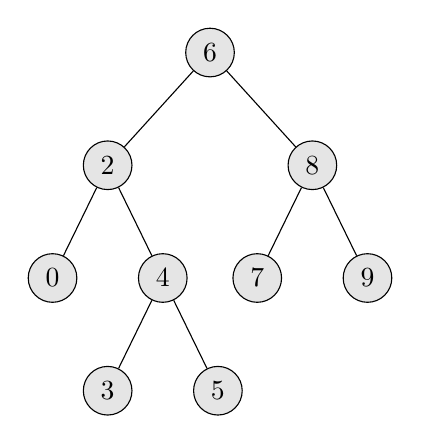
\begin{tikzpicture}
[mynode/.style={draw,circle,minimum size=5mm, fill=gray!20!}]
\node(){};
\node[mynode](1) {6};
\node[mynode](2)[below=8mm of 1, xshift=-13mm] {2};
\node[mynode](3)[below=8mm of 1, xshift=13mm] {8};
\node[mynode](4)[below=8mm of 2, xshift=-7mm] {0};
\node[mynode](5)[below=8mm of 2, xshift=7mm] {4};
\node[mynode](6)[below=8mm of 3, xshift=-7mm] {7};
\node[mynode](7)[below=8mm of 3, xshift=7mm] {9};
\node[mynode](8)[below=8mm of 5, xshift=-7mm] {3};
\node[mynode](9)[below=8mm of 5, xshift=7mm] {5};
\draw (1) -- (2);
\draw (1) -- (3);
\draw (2) -- (4);
\draw (2) -- (5);
\draw (3) -- (6);
\draw (3) -- (7);
\draw (5) -- (8);
\draw (5) -- (9);
\end{tikzpicture}
\end{figure}
$p = 2$, $q = 4$
\\
\textbf{Output}: 2
\\
\textbf{Explanation}: 
\\
The LCA of nodes 2 and 4 is 2, since a node can be a descendant of itself according to the LCA definition.
\end{flushleft}

\paragraph{Note:}

\begin{itemize}
\item All of the nodes' values will be unique.
\item $p$ and $q$ are different and both values will exist in the \texttt{BST}.
\end{itemize}
\subsection{BST Search}

借助\texttt{BST}的特性,由于题目中说明了每个节点的value都是unique的,所以
\begin{itemize}
\item 当根节点的value比$p$和$q$的value都大时,说明$p$和$q$的\texttt{LCA}在左子树,因此递归到左子树寻找。
\item 当根节点的value比$p$和$q$的value都大小时,说明$p$和$q$的\texttt{LCA}在右子树,因此递归到右子树寻找。
\item 否则,根节点的value处于$p$和$q$的value中间,因此根节点就是$p$和$q$的\texttt{LCA}。
\end{itemize}

\setcounter{lstlisting}{0}
\begin{lstlisting}[style=customc, caption={BST Properties}]
TreeNode* LCA( TreeNode* root, TreeNode* p, TreeNode* q )
{
    if( !root )
    {
        return root;
    }

    if( ( root->val > p->val ) && ( root->val > q->val ) )
    {
        //LCA in left subtree
        return LCA( root->left, p, q );
    }

    if( ( root->val < p->val ) && ( root->val < q->val ) )
    {
        //LCA in right subtree
        return LCA( root->right, p, q );
    }

    return root;
}

\end{lstlisting}
%\section{236 --- Lowest Common Ancestor of a Binary Tree}
Given a binary tree, find the lowest common ancestor (\texttt{LCA}) of two given nodes in the tree.
\par
According to the definition of \texttt{LCA} on \textbf{Wikipedia}: \textit{The lowest common ancestor is defined between two nodes $p$ and $q$ as the lowest node in $T$ that has both $p$ and $q$ as descendants (where we allow \textbf{a node to be a descendant of itself}).}

\paragraph{Example 1:}

\begin{flushleft}
\textbf{Input}: 
\begin{figure}[H]
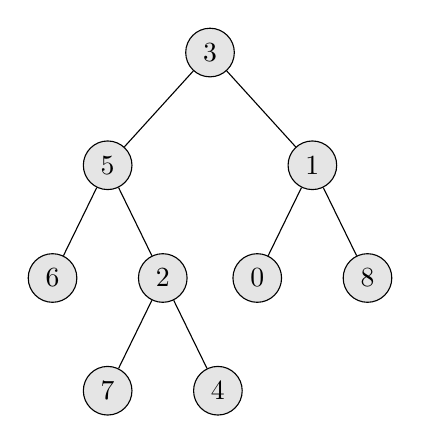
\begin{tikzpicture}
[mynode/.style={draw,circle,minimum size=5mm, fill=gray!20!}]
\node(){};
\node[mynode](1) {3};
\node[mynode](2)[below=8mm of 1, xshift=-13mm] {5};
\node[mynode](3)[below=8mm of 1, xshift=13mm] {1};
\node[mynode](4)[below=8mm of 2, xshift=-7mm] {6};
\node[mynode](5)[below=8mm of 2, xshift=7mm] {2};
\node[mynode](6)[below=8mm of 3, xshift=-7mm] {0};
\node[mynode](7)[below=8mm of 3, xshift=7mm] {8};
\node[mynode](8)[below=8mm of 5, xshift=-7mm] {7};
\node[mynode](9)[below=8mm of 5, xshift=7mm] {4};
\draw (1) -- (2);
\draw (1) -- (3);
\draw (2) -- (4);
\draw (2) -- (5);
\draw (3) -- (6);
\draw (3) -- (7);
\draw (5) -- (8);
\draw (5) -- (9);
\end{tikzpicture}
\end{figure}
$p = 5$, $q = 1$
\\
\textbf{Output}: 6
\\
\textbf{Explanation}: 
\\
The LCA of nodes 5 and 1 is 3.
\end{flushleft}

\paragraph{Example 2:}

\begin{flushleft}
\textbf{Input}:
\begin{figure}[H]
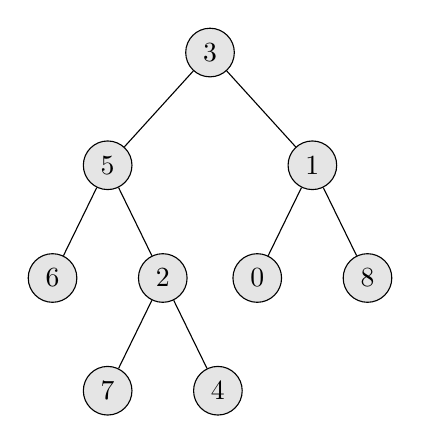
\begin{tikzpicture}
[mynode/.style={draw,circle,minimum size=5mm, fill=gray!20!}]
\node(){};
\node[mynode](1) {3};
\node[mynode](2)[below=8mm of 1, xshift=-13mm] {5};
\node[mynode](3)[below=8mm of 1, xshift=13mm] {1};
\node[mynode](4)[below=8mm of 2, xshift=-7mm] {6};
\node[mynode](5)[below=8mm of 2, xshift=7mm] {2};
\node[mynode](6)[below=8mm of 3, xshift=-7mm] {0};
\node[mynode](7)[below=8mm of 3, xshift=7mm] {8};
\node[mynode](8)[below=8mm of 5, xshift=-7mm] {7};
\node[mynode](9)[below=8mm of 5, xshift=7mm] {4};
\draw (1) -- (2);
\draw (1) -- (3);
\draw (2) -- (4);
\draw (2) -- (5);
\draw (3) -- (6);
\draw (3) -- (7);
\draw (5) -- (8);
\draw (5) -- (9);
\end{tikzpicture}
\end{figure}
$p = 5$, $q = 4$
\\
\textbf{Output}: 5
\\
\textbf{Explanation}: 
\\
The LCA of nodes 5 and 4 is 5, since a node can be a descendant of itself according to the LCA definition.
\end{flushleft}

\paragraph{Note:}

\begin{itemize}
\item All of the nodes' values will be unique.
\item $p$ and $q$ are different and both values will exist in the binary tree.
\end{itemize}
\subsection{Recursion}
这道题和235不同,这里只是一般的bianry tree。
\begin{itemize}
\item 按照深度优先的方式遍历tree。
\item 当遇到$p$或者$q$时,返回一些boolean flags。这些flags会帮助确定是否在某个path上找到了$p$或者$q$。
\item \texttt{LCA}则是其对其左右子树进行递归处理都能够返回\texttt{true}的那个节点。
\item 由于\texttt{LCA}也可能是$p$或者$q$中的一个,这种情况下只会有一个子树返回\texttt{true}
\end{itemize}
算法过程如下
\begin{itemize}
\item 从root开始遍历tree。
\item 如果current node本身就是$p$或者是$q$,将一个变量$x$设为\texttt{true},然后继续在左右子树中寻找另外一个节点。
\item 如果遍历左子树的结果$l$或者遍历右子树$r$是\texttt{true},表明$p$和$q$中的一个被找到了。
\item 在遍历过程中,任何时候发现$l$, $r$和$x$这三个变量中有两个为\texttt{true}了,表明已经找到了$p$和$q$的\texttt{LCA}。
\item 具体实现时,用$l$, $r$和$x$都设为\texttt{int}。这样可以通过判断这三个的和来判定是否有两个为\texttt{true}。
\end{itemize}
\setcounter{lstlisting}{0}
\begin{lstlisting}[style=customc, caption={Recursion}]
TreeNode* LCA( TreeNode* root, TreeNode* p, TreeNode* q )
{
    TreeNode* ans;
    dfs( root, p, q, ans );

    return ans;
}

bool dfs( TreeNode* node, TreeNode* p, TreeNode* q, TreeNode*& lca )
{
    if( !node )
    {
        return false;
    }

    int x = 0;

    if( ( node == p ) || ( node == q ) )
    {
        //one of p and q is found
        x = 1;
    }

    int l = 0;
    if( dfs( node->left, p, q, lca ) )
    {
        //Found p and/or q in left tree
        l = 1;
    }

    int r = 0;
    if( dfs( node->right, p, q, lca ) )
    {
        //Found p and/or q in right tree
        r = 1;
    }

    if( l + r + x >= 2 )
    {
        //LCA is found
        lca = node;
    }

    return ( l + r + x ) > 0; //at least find one of p and q
}
\end{lstlisting}
\subsection{Another Recursion}
\begin{CJK*}{UTF8}{gbsn}
在binary tree中搜索$p$和$q$,然后从遍历路径中找到最后一个相同的节点即为\texttt{LCA}。边界情况很简单: 首先看当前结点是否为\texttt{null},若为\texttt{null}则直接返回\texttt{null},若为$p$或$q$中的任意一个,直接返回当前结点
\par
如果当前结点不等于$p$或$q$,$p$和$q$要么分别位于左右子树中,要么同时位于左子树,或者同时位于右子树
\begin{itemize}
\item 若$p$和$q$分别位于左右子树中,那么对左右子结点进行recursion,会分别返回$p$和$q$结点的位置,而当前结点正好就是$p$和$q$的最小共同父结点,直接返回当前结点即可,这就是题目中的例子1的情况。
\item 若$p$和$q$同时位于左子树,这时候调用递归函数处理right subtree会返回\texttt{null}, 而处理left subtree有两种情况,
\begin{enumerate}
\item 函数返回的是$p$和$q$中靠近根节点的那个节点,这时候返回这个节点。这就是题目中的例子2的情况。
\item 函数返回的是$p$和$q$的\texttt{LCA},就是说当前结点的左子树中的某个结点才是$p$和$q$的\texttt{LCA},也直接返回这个结果。
\end{enumerate}
\item 若$p$和$q$同时位于右子树,和上述左子树情形类似。
\end{itemize}
\end{CJK*}
\begin{lstlisting}[style=customc, caption={Recursion Based On Left And Right Subtree}]
TreeNode* LCA( TreeNode* root, TreeNode* p, TreeNode* q )
{
    if( !root || root == p || root == q )
    {
        return root;
    }

    //process left subtree
    auto l_node = LCA( root->left, p, q );
    //process right subtree
    auto r_node = LCA( root->right, p, q );

    //found the two nodes in left and right subtree respectively
    //LCA is found
    if( l_node && r_node )
    {
        return root;
    }

    //p and q only in left subtree
    if( l_node )
    {
        return l_node;
    }

    //p and q only in right subtree
    return r_node;
}
\end{lstlisting}
\subsection{Iterative using parent pointers}
\begin{CJK*}{UTF8}{gbsn}
这种方法则需要借助queue和hash map来寻找最接近$p$和$q$的common ancestor。
\par
算法步骤如下
\begin{enumerate}
\item 从根节点开始遍历tree。由于是iterative traverse,所以需要借助queue。
\item 将当前节点的parent node保存在一个hash map $M$中直到找到$p$和$q$。
\item 一旦找到$p$和$q$,将$p$的所有ancestors从$M$中加入到一个hash set $S$中。
\item 然后在$M$中遍历$q$所有的ancestors。如果当前遇到的ancestor可以在$S$中找到,这就是$p$和$q$的\texttt{LCA}。
\end{enumerate}
\end{CJK*}
\begin{lstlisting}[style=customc, caption={Iterative Searching}]
TreeNode* LCA( TreeNode* root, TreeNode* p, TreeNode* q )
{

    queue<TreeNode*> qt;
    unordered_map<TreeNode*, TreeNode*> m;

    qt.push( root );
    m.emplace( root, nullptr ); //root's parent is empty

    //iterative traverse the tree using the queue
    while( !qt.empty() )
    {
        auto it_p = m.find( p );
        auto it_q = m.find( q );

        if( ( it_p != m.end() ) && ( it_q != m.end() ) )
        {
            //p and q both are found
            break;
        }

        auto t = qt.front();
        qt.pop();

        if( t->left )
        {
            m.emplace( t->left, t );
            qt.emplace( t->left );
        }

        if( t->right )
        {
            m.emplace( t->right, t );
            qt.emplace( t->right );
        }
    }

    unordered_set<TreeNode*> A;

    // add all p's ancestors into the hash set A
    auto t = p;
    while( t )
    {
        A.insert( t );
        t = m[t];
    }

    // find the first ancestor of q that
    // can be found in A
    t = q;
    while( t )
    {
        auto it = ancestors.find( t );

        if( it != ancestors.end() )
        {
            return *it;
        }

        t = m[t];
    }

    // cannot find LCA
    return nullptr;
}
\end{lstlisting}

%\section{237 --- Delete Node in a Linked List}
Write a function to delete a node (except the tail) in a singly linked list, given only access to that node.

\paragraph{Example 1:}

\textbf{Input}:\fcj{ head = [4,5,1,9]}, \fcj{node = 5}

\textbf{Output}: \fcj{[4,1,9]}

\textbf{Explanation}: 

You are given the second node with value 5, the linked list should become \fcj{4 -> 1 -> 9} after calling your function.

\paragraph{Example 2:}

\textbf{Input}: \fcj{head = [4,5,1,9]}, \fcj{node = 1}

\textbf{Output}: \fcj{[4,5,9]}

\textbf{Explanation}: 

You are given the third node with value 1, the linked list should become \fcj{4 -> 5 -> 9} after calling your function.
 

\paragraph{Note:}

\begin{itemize}
\item The linked list will have at least two elements.
\item All of the nodes' values will be unique.
\item The given node will not be the tail and it will always be a valid node of the linked list.
\item Do not return anything from your function.
\end{itemize}

\subsection{Swap}
Copy the next node's value to the deleted node and delete next node.

\setcounter{lstlisting}{0}
\begin{lstlisting}[style=customc, caption={Swap}]
void deleteNode( ListNode* node )
{
    //copy node->next's value
    //to node
    auto p( node->next );
    node->val = p->val;
    //delete node->next
    node->next = p->next;
    p->next = nullptr;
    delete p;
}
\end{lstlisting}
%\section{238 --- Product of Array Except Self}
Given an array $A$ of $n$ integers where $n > 1$,  return an array $B$ such that B[i] is equal to the product of all the elements of $A$ except $A[i]$.

\paragraph{Example:}
\begin{flushleft}
\textbf{Input}:  $[1,2,3,4]$
\\
\textbf{Output}: $[24,12,8,6]$
\end{flushleft}

\paragraph{Note:}
\begin{itemize}
\item Please solve it without division and in O(n).
\end{itemize}

\paragraph{Follow up:}
\begin{itemize}
\item Could you solve it with constant space complexity? (The output array $B$ does not count as extra space for the purpose of space complexity analysis.)
\end{itemize}
\subsection{Simplify Prefix And Postfix Product Array To Two Variables}
\begin{CJK*}{UTF8}{gbsn}
\begin{itemize}
\item 如果用prefix and postfix product array,就很简单了,从左到右逐个获得prefix product。然后再从右到左逐个获得postfix product,两个相乘就是所在index的product except itself。
\item 但其实可以将prefix and postfix product array简化成两个变量,因为我们只关心上一个值。
\end{itemize}
\end{CJK*}
\setcounter{algorithm}{0}
\begin{algorithm}[H]
\caption{Prefix And Postfix Products}
\begin{algorithmic}[1]
\Procedure{ProductExceptSelf}{$A, L$}
\State $\star$ Initialize $\alpha$ and $\beta$ as ones. $\alpha$ will save the prefix products while $\beta$ for postfix products.
\State $\star$ Initialize $P$ as the result array. $P$ has length $L$ and all values are initialized to 1.
\State $\ast$ Start the process of finding prefix and postfix products
\For{$i:=0$ \textbf{to} $L-1$}
\State $P[i]\gets P[i] \times \alpha$
\State $\alpha\gets \alpha\times A[i]$ \Comment Update prefix product
\State \Return $P$
\algstore{238algo}
\end{algorithmic}
\end{algorithm}
\begin{algorithm}[H]
\begin{algorithmic}[1]
\algrestore{238algo}
\State $j:=L-i-1$ \Comment We needs to get postfix product at same time
\State $P[j]\gets P[j]\times\beta$ 
\State $\beta\gets\beta\times A[j]$
\EndFor
\EndProcedure
\end{algorithmic}
\end{algorithm}
\begin{CJK*}{UTF8}{gbsn}
\paragraph{Note}
\begin{itemize}
\item 上述算法中,最开始其实$P[i]$和$P[j]$都不是正确的值,但是由于我们是同时从两边进行更新,因此循环结束后就会得到正确的值。
\end{itemize}
\end{CJK*}
\setcounter{lstlisting}{0}
\begin{lstlisting}[style=customc, caption={Prefix And Postfix Product}]
vector<int> productExceptSelf( vector<int>& nums )
{
    int alpha = 1;
    int beta = 1;

    vector<int> P( nums.size(), 1 );

    for( size_t i = 0; i < nums.size(); ++i )
    {
        //get prefix product
        P[i] *= alpha;
        alpha *= nums[i];

        //prcocess postfix product
        auto j = nums.size() - i - 1;
        P[j] *= beta;
        beta *= nums[j];
    }

    return P;
}
\end{lstlisting}
%\section{239 --- Sliding Window Maximum}
Given an array $A$, there is a sliding window of size $k$ which is moving from the very left of the array to the very right. You can only see the $k$ numbers in the window. Each time the sliding window moves right by one position. Return the \texttt{max} sliding window.

\paragraph{Example:}
\begin{flushleft}
\textbf{Input}: \fcj{A = [1,3,-1,-3,5,3,6,7]}, and $k = 3$
\\
\textbf{Output}: \fcj{[3,3,5,5,6,7]}
\\
\textbf{Explanation:} 
\begin{itemize}
\item $[1,\;  3,\;  -1],\; -3,\;  5,\;  3,\;  6,\;  7 \Longrightarrow       3$
\item $1,\; [3,\;  -1,\;  -3,\;] 5,\;  3,\;  6,\;  7 \Longrightarrow       3$
\item $1,\;  3,\; [-1,\;  -3,\;  5],\; 3,\;  6,\;  7 \Longrightarrow 5$
\item $1,\; 3,\; -1,\;[-3,\; 5,\; 3],\; 6,\; 7 \Longrightarrow 5$
\item $1,\;  3,\;  -1,\;  -3,\; [5,\;  3,\;  6],\; 7 \Longrightarrow       6$
\item $1,\; 3,\; -1,\;  -3,\;  5,\; [3,\;  6,\;  7]  \Longrightarrow  7$
\end{itemize}
\end{flushleft}
\paragraph{Note:}
\begin{itemize}
\item You may assume $k$ is always valid, $1 \leq k \leq$ input array's size for non-empty array.
\end{itemize}
\paragraph{Follow up:}
\begin{itemize}
\item Could you solve it in linear time?
\end{itemize}
\subsection{Double-End Queue}
所有的固定长度滑动窗口问题都有可以用double-end queue来作为基础的数据结构。
\begin{itemize}
\item 遍历数组$A$。用一个double-end queue $q$来存放访问的index
。
\item 在当前index $i$,如果$q$的\texttt{front}刚好等于$i-k$,那么就将\texttt{front}从$q$中去除。因为这时候滑动窗口已经不再包含距离大于$k$的元素了。
\item 然后进入一个循环比较$q$的\texttt{back}是否小于或者等于当前数字,如果小于或者等于,一直将\texttt{back}从$q$中移除。
\item 然后将$i$加入到$q$的后面。
\item 如果$i\geq k$,这时候就要输出最大值了,而最大值就是$q$的front。
\end{itemize}

\setcounter{lstlisting}{0}
\begin{lstlisting}[style=customc, caption={Deque}]
vector<int> maxSlidingWindow( vector<int>& nums, int k )
{
    int L = static_cast<int>( nums.size() );
    deque<int> q;
    vector<int> m;
    m.reserve( L - k + 1 );
    for( int i = 0; i < L; ++i )
    {
        //pop out index outside sliding window
        if( !q.empty() && ( q.front() == i - k ) )
        {
            q.pop_front();
        }
        //pop out back index where numbers are no larger than
        //current number
        while( !q.empty() && ( nums[q.back()] <= nums[i] ) )
        {
            q.pop_back();
        }
        //add current index to q's back end
        q.push_back( i );
        // need to output maximum of sliding window
        // from k-1 to L-1
        if( i >= k - 1 )
        {
            m.push_back( nums[q.front()] );
        }
    }
    return m;
}
\end{lstlisting}
%\section{240 --- Search a 2D Matrix II}
Write an efficient algorithm that searches for a value in an $m \times n$ matrix $M$. This matrix has the following properties:
\begin{itemize}
\item Integers in each row are sorted in ascending from left to right.
\item Integers in each column are sorted in ascending from top to bottom.
\end{itemize}

\paragraph{Example:}
\begin{flushleft}
Consider the following matrix:
\begin{table}[H]
\begin{tabular}{lllll}
1  & 4  & 7  & 11 & 15 \\
2  & 5  & 8  & 12 & 19 \\
3  & 6  & 9  & 16 & 22 \\
10 & 13 & 14 & 17 & 24 \\
18 & 21 & 23 & 26 & 30
\end{tabular}
\end{table}
Given target = 5, return \texttt{true}.
\\
Given target = 20, return \texttt{false}.
\end{flushleft}

\section{241 --- Different Ways to Add Parentheses}
Given a string of numbers and operators, return all possible results from computing all the different possible ways to group numbers and operators. The valid operators are $+$, $-$ and $\times$.

\paragraph{Example 1:}
\begin{flushleft}
Input: $2-1-1$
\\
Output: $[0, 2]$
\\
Explanation: 
\\
$((2-1)-1) = 0$
\\
$(2-(1-1)) = 2$
\end{flushleft}

\paragraph{Example 2:}
\begin{flushleft}
Input: $2\times3-4\times5$
\\
Output: $[-34, -14, -10, -10, 10]$
\\
Explanation:
\\ 
$(2\times(3-(4\times5))) = -34 $
\\
$((2\times3)-(4\times5)) = -14 $
\\
$((2\times(3-4))\times5) = -10 $
\\
$(2\times((3-4)\times5)) = -10 $
\\
$(((2\times3)-4)\times5) = 10$
\end{flushleft}
\subsection{Recursion}
\begin{itemize}
\item 遍历输入数组,每次遇到操作符号时,就从这个地方分成左右两个部分。
\item 分别对左右两个部分进行递归,返回结果就是各个部分运算得到的结果数组
\item 将两个数组中的结果两两组合即得到当前该操作符的所有运算结果。
\item 如果输入字符串只包含数字,则将该数字作为输出数组中的唯一元素。
\item 可以用memorize的方法减少重复的搜索。
\end{itemize}
\setcounter{lstlisting}{0}
\begin{lstlisting}[style=customc, caption={Recursion Without Memorization}]
vector<int> diffWaysToCompute( string input )
{
    vector<int> results;

    int num = 0;

    for( size_t i = 0; i < input.size(); ++i )
    {
        auto c = input[i];

        //if input has only number, num will be the number
        if( ( c >= '0' ) && ( c <= '9' ) )
        {
            num = num * 10 + ( c - '0' );
            continue;
        }

        //we break input into two parts
        //and recursively apply function to the two parts
        vector<int> left = diffWaysToCompute( input.substr( 0, i ) );
        vector<int> right = diffWaysToCompute( input.substr( i + 1 ) );

        //calculate results from the output arrays
        calc( left, right, results, c );

        num = 0;
    }

    // input contains only number
    if( results.empty() )
    {
        results.push_back( num );
    }

    return results;
}


void calc( vector<int>& left, vector<int>& right, vector<int>& results, char oper )
{
    if( oper == '*' )
    {
        for( auto l : left )
        {
            for( auto r : right )
            {
                results.push_back( l * r );
            }
        }
    }
    else if( oper == '-' )
    {
        for( auto l : left )
        {
            for( auto r : right )
            {
                results.push_back( l - r );
            }
        }
    }
    else if( oper == '+' )
    {
        for( auto l : left )
        {
            for( auto r : right )
            {
                results.push_back( l + r );
            }
        }
    }
}
\end{lstlisting}


\begin{lstlisting}[style=customc, caption={String View}]
vector<int> diffWaysToCompute( string input )
{
    return dfs( input );
}
vector<int> dfs( string_view sv )
{
    int num = 0;
    vector<int> vec_res;
    for( size_t i = 0; i < sv.size(); ++i )
    {
        auto c = sv[i];
        if( ( c >= '0' ) && ( c <= '9' ) )
        {
            num = num * 10 + ( c - '0' );
        }
        else
        {
            //recursive on left and right
            auto lhs = dfs( sv.substr( 0, i ) );
            auto rhs = dfs( sv.substr( i + 1 ) );
            if( c == '+' )
            {
                combine( lhs, rhs, vec_res, std::plus<int>() );
            }
            else if( c == '-' )
            {
                combine( lhs, rhs, vec_res, std::minus<int>() );
            }
            else
            {
                combine( lhs, rhs, vec_res, std::multiplies<int>() );
            }
            //reset num to zero
            num = 0;
        }
    }
    //if there is only number
    //add number to the result
    if( vec_res.empty() )
    {
        vec_res.push_back( num );
    }
    return vec_res;
}
//generate all possible results
template<typename F>
void combine( vector<int>& lhs, vector<int>& rhs, vector<int>& res, F f )
{
    for( int l : lhs )
    {
        for( int r : rhs )
        {
            res.push_back( f( l, r ) );
        }
    }
}
\end{lstlisting}
%\section{242 --- Valid Anagram}
Given two strings \fcj{s} and \fcj{t} , write a function to determine if  \fcj{t} is an anagram of  \fcj{s}.

\paragraph{Example 1:}

\begin{flushleft}
\textbf{Input}: \fcj{s = "anagram"}, \fcj{t = "nagaram"}

\textbf{Output}: \fcj{true}

\end{flushleft}

\paragraph{Example 2:}

\begin{flushleft}
\textbf{Input}: \fcj{s = "rat"}, \fcj{t = "car"}

\textbf{Output}: \fcj{false}

\end{flushleft}

\paragraph{Note:}

\begin{itemize}
\item You may assume the string contains only lowercase alphabets.
\end{itemize}

\paragraph{Follow up:}
\begin{itemize}
\item What if the inputs contain unicode characters? How would you adapt your solution to such case?
\end{itemize}

\subsection{Counter}

\setcounter{lstlisting}{0}
\begin{lstlisting}[style=customc, caption={Counter}]
bool isAnagram( string s, string t )
{
    //anagram strings must be equal size
    if( s.size() != t.size() )
    {
        return false;
    }
    int m[26] = {0};
    for( auto c : s )
    {
        m[c - 'a'] += 1;
    }
    for( auto c : t )
    {
        m[c - 'a'] -= 1;
        if( m[c - 'a'] < 0 )
        {
            //don't have same count of same letter
            return false;
        }
    }
    return true;
}
\end{lstlisting}

For unicode string, use a hash table instead of a fixed size counter. 
%\section{243 --- Shortest Word Distance}
Given a list of words and two words \fcj{word1} and \fcj{word2}, return the shortest distance between these two words in the list.

For example, Assume that words are 

\fcj{["practice", "makes", "perfect", "coding", "makes"]}.

\begin{flushleft}

\textbf{Input}: \fcj{word1 = "coding"}, \fcj{word2 = "practice"}

\textbf{Output}: 3

\textbf{Input}: \fcj{word1 = "makes"}, \fcj{word2 = "coding"}

\textbf{Output}: 1
\end{flushleft}

\paragraph{Note:}
\begin{itemize}
\item You may assume that \fcj{word1} \textbf{does not equal to} \fcj{word2}, and \fcj{word1} and \fcj{word2} are both in the list.
\end{itemize}

\subsection{One Pass}
We store the most recent locations of \fcj{word1} and \fcj{word2}. Each time we find a new occurrence of one of the words, update the result.

\setcounter{lstlisting}{0}
\begin{lstlisting}[style=customc, caption={One Pass}]
int shortestDistance( vector<string>& words, string word1, string word2 )
{
    auto L = static_cast< int >( words.size() );
    int p1 = -1;
    int p2 = -1;
    int ans = L;
    for( int i = 0; i < L; ++i )
    {
        if( word1 == words[i] )
        {
            p1 = i;
        }
        else if( word2 == words[i] )
        {
            p2 = i;
        }
        if( ( p1 >= 0 ) && ( p2 >= 0 ) )
        {
            //update minimum distance
            ans = ( min )( ans, ( abs )( p2 - p1 ) );
        }
    }
    return ans;
}
\end{lstlisting} %$
%\section{244 --- Shortest Word Distance II}
This is a follow up of \textbf{242 --- Shortest Word Distance}. The only difference is now you are given the list of words and your method will be called repeatedly many times with different parameters. How would you optimize it?
\par
Design a class which receives a list of words $W$ in the constructor, and implements a method that takes two words $A$ and $B$ and return the shortest distance between these two words in the list.
\par
For example,
\par
Assume that $W = [\texttt{practice}, \texttt{makes}, \texttt{perfect}, \texttt{coding}, \texttt{makes}]$.
\par
Given $A = \texttt{coding}$, $B = \texttt{practice}$, return 3.
\par
Given $A = \texttt{makes}$, $B = \texttt{coding}$, return 1.
\paragraph{Note:}
\begin{itemize}
\item You may assume that $A$ does not equal to $B$, and $A$ and $B$ are both in the list.
\end{itemize} %$
%\section{245 --- Shortest Word Distance III}
This is a follow up of \textbf{242 --- Shortest Word Distance}. The only difference is now $A$ could be the same as $B$.
\par
Given a list of words $W$ and two words $A$ and $B$, return the shortest distance between these two words in the list.
\par
$A$ and $B$ may be the same and they represent two individual words in the list.
\par
For example,
\par
Assume that $W = [\texttt{practice}, \texttt{makes}, \texttt{perfect}, \texttt{coding}, \texttt{makes}]$.
\par
Given $A = \texttt{makes}$, $B = \texttt{coding}$, return 1.
\par
Given $A = \texttt{makes}$, $B = \texttt{makes}$, return 3.
\paragraph{Note:}
\begin{itemize}
\item You may assume $A$ and $B$ are both in the list.
\end{itemize}

\subsection{One Pass}
Similar to problem \textbf{243}. For the same string, just record last index and get the maximum difference of adjacent ones. %$
%\section{246 --- Strobogrammatic Number}
A strobogrammatic number is a number that looks the same when rotated 180 degrees (looked at upside down).
\par
Write a function to determine if a number is strobogrammatic. The number is represented as a string.

\paragraph{Example 1:}
\begin{flushleft}
\textbf{Input}:  69
\\
\textbf{Output}: \texttt{true}
\end{flushleft}

\paragraph{Example 2:}
\begin{flushleft}
\textbf{Input}:  88
\\
\textbf{Output}: \texttt{true}
\end{flushleft}

\paragraph{Example 3:}
\begin{flushleft}
\textbf{Input}:  962
\\
\textbf{Output}: \texttt{false}
\end{flushleft}

\subsection{Replace And Reverse}

\setcounter{lstlisting}{0}
\begin{lstlisting}[style=customc, caption={Replace And Reverse}]
bool isStrobogrammatic( string num )
{
    string y( num );
    unordered_map<char, char> m =
    {
        { '6', '9' },
        {'9', '6'},
        {'8', '8'},
        {'1', '1'},
        {'0', '0'}
    };
    for( auto& c : y )
    {
        auto it = m.find( c );
        if( it == m.end() )
        {
            //cannot get valid letter
            return false;
        }
        c = it->second;
    }
    //we need to reverse the generated string
    reverse( begin( y ), end( y ) );
    return y == num;
}
\end{lstlisting} %$
%\section{247 --- Strobogrammatic Number II}
A strobogrammatic number is a number that looks the same when rotated 180 degrees (looked at upside down).
\par
Find all strobogrammatic numbers that are of length $n$.
\par
For example,
\par
Given $n = 2$, return $[11,\;69,\;88,\;96]$.
\par
\paragraph{Hint:}
\begin{itemize}
\item Try to use recursion and notice that it should recurse with $n - 2$ instead of $n - 1$.
\end{itemize}
 %$
%\section{248 --- Strobogrammatic Number III}
A strobogrammatic number is a number that looks the same when rotated 180 degrees (looked at upside down).

Write a function to count the total strobogrammatic numbers that exist in the range of $[L,H]$

\paragraph{Example:}
\begin{flushleft}
Input: $L = 50$, $H = 100$

Output: 3 

Explanation: 69, 88, and 96 are three strobogrammatic numbers.
\end{flushleft}

\paragraph{Note:}
\begin{itemize}
\item Because the range might be a large number, $L$ and $H$ numbers are represented as string.
\end{itemize}


\subsection{Recursion}
The solution is based on problem \textbf{247}: We don't save the result but counting inside the recursion process.

We need to initialize cases for $n=0$ and $n=1$. Then starting the recursion from \fcc{low} to \fcc{high}. 

\setcounter{lstlisting}{0}
\begin{lstlisting}[style=customc, caption={Recursion}]
int strobogrammaticInRange( string low, string high )
{
    long ans = 0;
    dfs( low, high, "", ans );
    dfs( low, high, "0",  ans );
    dfs( low, high, "1", ans );
    dfs( low, high, "8",  ans );
    return ans;
}

void dfs( string_view lo, string_view hi, string s, long& ans )
{
    auto sz = s.size();
    if( ( sz <= hi.size() ) && ( sz >= lo.size() ) )
    {
        if( ( sz == hi.size() ) && ( s.compare( hi ) > 0 ) )
        {
            return;
        }
        if( ( sz > 1ull ) && ( s[0] == '0' ) )
        {
            //we cannot return here
            //since we can still try next
        }
        else if( ( sz == lo.size() ) && ( s < lo ) )
        {
            //we cannot return here
            //since we can still try next
        }
        else
        {
            ++ans;
        }
    }
    if( sz + 2ull > hi.size() )
    {
        //no need to try if add two letters
        //exceed the size of high
        return;
    }
    dfs( lo, hi, "0" + s + "0", ans );
    dfs( lo, hi, "1" + s + "1", ans );
    dfs( lo, hi, "8" + s + "8", ans );
    dfs( lo, hi, "6" + s + "9", ans );
    dfs( lo, hi, "9" + s + "6", ans );
}
\end{lstlisting} %$
%\section{249 --- Group Shifted Strings}
Given a string $S$, we can \texttt{shift} each of its letter to its successive letter, for example: $\texttt{abc} \longrightarrow \texttt{bcd}$. We can keep \texttt{shifting} which forms the sequence:
\par
$\texttt{abc} \longrightarrow \texttt{bcd} \longrightarrow \ldots \longrightarrow \texttt{xyz}$
\par
Given a list of strings $A$ which contains only lowercase alphabets, group all strings that belong to the same shifting sequence.
\par
For example, given: 
$[\texttt{abc},\; \texttt{bcd},\; \texttt{acef},\; \texttt{xyz},\; \texttt{az},\; \texttt{ba},\; \texttt{a},\; \texttt{z}]$,
\par
Return:
\begin{table}[H]
\begin{tabular}{l}
$\texttt{abc},\;\texttt{bcd},\;\texttt{xyz}$ \\
$\texttt{az},\;\texttt{ba}$\\
\texttt{acef}\\
$\texttt{a},\;\texttt{z}$
\end{tabular}
\end{table}

\paragraph{Note:} 
\begin{itemize}
\item For the return value, each inner list's elements must follow the lexicographic order.
\end{itemize}
\subsection{Unique Distance}
注意到shift的字符串中其实每个字母和首字符的相对差都是相等的,比如\fcj{abc}和\fcj{efg}互为shift strings,对于\fcj{abc}来说,$b$和$a$的差是1,$c$和$a$的差是2,对于\texttt{efg}来说,$f$和$e$的difference是1,$g$和$e$的difference是2。利用这个特性就能很好的对字符串进行分组了。

技巧就是用每个字符串中每个字符和首字符的difference构成一个key,然后用这个key作为group string的依照。比如\fcj{abc}的每个字符和首字符的difference构成的key为$012$,然后用$012$这个key去判断哪些字符也具有这个key。

在coding时,这个key可以转换成字符串。以避免形成0开头的数字所带来的重复key的问题。

另外,由于题目要求是按照字典顺序,同时考虑到可能存在重复的字符串,因此用multiset来存放相同的字符串。

\setcounter{lstlisting}{0}
\begin{lstlisting}[style=customc, caption={Unique Distance}]
vector<vector<string>> groupStrings( vector<string>& strings )
{
 vector<vector<string>> groupStrings( vector<string>& strings )
{
    unordered_map<string, vector<string_view>> dict;
    for( const auto& s : strings )
    {
        string key;
        for( size_t i = 1; i < s.size(); ++i )
        {
            //make sure the difference between
            //current letter and the first letter
            //is positive number
            key += to_string( ( s[i] - s[0] + 26 ) % 26 );
            key.push_back( '#' );
        }
        dict[key].emplace_back( s.c_str(), s.size() );
    }
    vector<vector<string>> ans;
    for( const auto& p : dict )
    {
        ans.emplace_back( begin( p.second ), end( p.second ) );
    }
    return ans;
}
\end{lstlisting} %$
%\section{250 --- Count Univalue Subtrees}
Given a binary tree, count the number of uni-value subtrees.
\par
A Uni-value subtree means all nodes of the subtree have the same value.
\par
For example:
\begin{flushleft}
\textbf{Input}:
\begin{figure}[H]
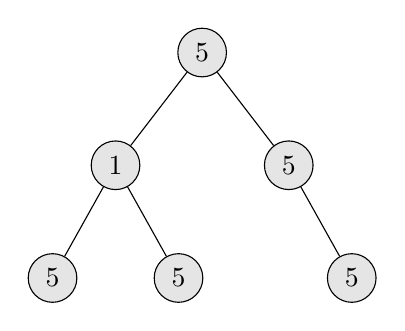
\begin{tikzpicture}
[mynode/.style={draw,circle,minimum size=5mm, fill=gray!20!}]
\node(){};
\node[mynode](A) {5};
\node[mynode](D)[below=8mm of A, xshift=-11mm] {1};
\node[mynode](E)[below=8mm of A, xshift=11mm] {5};
\node[mynode](X)[below=8mm of D, xshift=-8mm] {5};
\node[mynode](Y)[below=8mm of D, xshift=8mm] {5};
\node[mynode](Z)[below=8mm of E, xshift=8mm] {5};
\draw (A) -- (D);
\draw (A) -- (E);
\draw (D) -- (X);
\draw (D) -- (Y);
\draw (E) -- (Z);
\end{tikzpicture}
\end{figure}
\textbf{Output}: 4
\end{flushleft}
\subsection{Recursion On Every Node}
先序遍历树的所有的节点,然后对每一个节点调用判断以当前节点为根的字数的所有节点是否相同。
\begin{itemize}
\item 需要一个function检查以当前节点为根节点的tree是否是uni-value tree。
\item 另外需要一个辅助函数进行递归处理,以得到uni-value tree的个数。
\end{itemize}


\setcounter{lstlisting}{0}
\begin{lstlisting}[style=customc, caption={Recursive On Each NOde}]
int countUnivalSubtrees( TreeNode* root )
{
    int ans = 0;

    dfs( root, ans );

    return ans;
}

void dfs( TreeNode* node, int &ans )
{
    if( !node )
    {
        return;
    }

    if( is_unival( node, node->val ) )
    {
        //Found a uni-value tree
        ++ans;
    }

    dfs( node->left, ans );
    dfs( node->right, ans );
}

bool is_unival( TreeNode* node, int val )
{
    if( !node )
    {
        return true;
    }

    if( node->val != val )
    {
        return false;
    }

    if( !is_unival( node->left, node->val ) )
    {
        return false;
    }

    if( !is_unival( node->right, node->val ) )
    {
        return false;
    }

    return true;
}
\end{lstlisting}
\subsection{Recursion}
上述解法不是很高效,含有大量的重复check。可以采用如下方法进行优化
\begin{itemize}
\item 采用后序遍历的顺序,
\item 对于当前遍历到的节点,如果对其左右子节点分别递归调用函数,返回均为\fcc{true},那么说明当前节点的值和左右子树的值都相同,因此找到了一个以当前节点为根节点的uni-value tree。
\item 由于递归函数返回当前树是不是uni-value tree,因此判断当前节点的value和给定的value是否相同。
\item 这就相当于把上述的\texttt{DFS}和\texttt{IsUnival}进行合并。
\item 区别在与,这时候,无论左右子树递归结果如何,我们都要在对这两个子树做完递归调用后,再确定是否返回\fcc{true}/\fcc{false}。否则如果在进行完左子树调用后,发现不是uni-value tree就立刻返回\fcc{false},就会skip 右子树的检查了。
\item 最后由于返回的是当前节点的值和其父节点的值是否相等,对于整个树的root node,这个值设为一个和root node的值不相同的数。
\end{itemize}

\begin{lstlisting}[style=customc,caption={More Efficient Recursive Approach}]
{
    int ans = 0;

    is_unival( root, -1, ans );

    return ans;
}

bool is_unival( TreeNode* node, int val, int& ans )
{
    if( !node )
    {
        return true;
    }

    //we must do the recursive processing for both subtrees
    bool b_left = is_unival( node->left, node->val, ans );
    bool b_right = is_unival( node->right, node->val, ans );

    if( !b_left || !b_right )
    {
        return false;
    }

    ++ans;

    return node->val == val;
}
\end{lstlisting} %$
\section{251 --- Flatten 2D Vector}
Implement an iterator to flatten a 2d vector.
\par
For example,
\par
Given 2d vector = $[[1,2],\;[3],\;[4,5,6]]$
\par
By calling \texttt{next} repeatedly until \texttt{hasNext} returns \texttt{false}, the order of elements returned by \texttt{next} should be: 
\par

$[1,2,3,4,5,6]$.
\par
\texttt{Hint:}

\begin{itemize}
\item How many variables do you need to keep track?
\item Two variables is all you need. Try with $x$ and $y$.
\item Beware of empty rows. It could be the first few rows.
\item To write correct code, think about the invariant to maintain. What is it?
\item The invariant is $x$ and $y$ must always point to a valid point in the 2d vector. Should you maintain your invariant ahead of time or right when you need it?
\item Not sure? Think about how you would implement \texttt{hasNext}(). Which is more complex?
\item Common logic in two different places should be refactored into a common method.
\end{itemize}

\paragraph{Follow up:}
\begin{itemize}
\item As an added challenge, try to code it using only iterators in \texttt{C++} or iterators in \texttt{Java}.
\end{itemize}
\subsection{Iterator}
将$x$定义为row的iterator,再用另外一个变量$z$指向二维数组的末尾,同时定义一个整型变量$y$来指向列位置
\setcounter{lstlisting}{0}
\begin{lstlisting}[style=customc, caption={Iterator}]
class Vector2D
{
public:
    Vector2D( vector<vector<int>>& vec2d )
    {
        x = vec2d.begin();
        z = vec2d.end();
    }
	
    int next()
    {
        return ( *x )[y++];
    }
	
    bool hasNext()
    {
        if( ( x != z ) && ( y == ( *x ).size() ) )
        {
            ++x;
            y = 0;
        }
        return x != z;
    }

private:
    vector<vector<int>>::iterator x;
    vector<vector<int>>::iterator z;
    size_t y = 0;
};
\end{lstlisting} %$
\section{252 --- Meeting Rooms}
Given an array of meeting time intervals $A$ consisting of start and end times $[s_1,\;e_1],\;[s_2,\;e_2],\;\ldots$ $(s_i < e_i)$, determine if a person could attend all meetings.
\par
\begin{flushleft}
\textbf{Input}: $A =[[0, 30],\;[5, 10],\;[15, 20]]$
\\
\textbf{Output}: \texttt{false}
\end{flushleft}
\subsection{Check Overlapped Ranges}
很简单的题目,将输入的ranges按照start time从小到打排序,然后依次看上一个range的end是否小于或者等于下一个range的start time。 %$
\section{253 --- Meeting Rooms II}
Given an array of meeting time intervals $A$ consisting of start and end times $[s_1,\;e_1],\;[s_2,\;e_2],\;\ldots$ $(s_i < e_i)$, find the minimum number of conference rooms required.
\par
\begin{flushleft}
\textbf{Input}: $A =[[0, 30],\;[5, 10],\;[15, 20]]$
\\
\textbf{Output}: 2
\end{flushleft}
\subsection{Tree Map}
\begin{itemize}
\item Tree Map能够自动排序插入的数
\item 遍历$A$,同时maintain一个tree map $M$
\begin{itemize}
\item 遇到start,将其插入$M$,对应的值设为$1$,如果已经存在将其对应的value加1
。
\item 遇到end,将其拆入$M$,对应的值设为$-1$。如果这个end在$M$中存在,将其对应的value减1。
\end{itemize}
\item 然后遍历$M$,累加各个key的value,同时maintain一个计数器,如果发生overlap,那么这个计数器的值在一直增加。
\item 记录遍历过程中计数器的最大值,这个最大值就是overlap的最多的interval的个数。
\end{itemize}
\setcounter{algorithm}{0}
\begin{algorithm}[H]
\caption{Counter Of Overlapped Intervals}
\begin{algorithmic}[1]
\Procedure{MinMeetingRooms}{$A, L$}
\State $\star$ 创建一个Tree Map $M$
\For{$i:=0$ \textbf{to} L-1}
\State $\star$ 将$A[i]$的\texttt{start}插入$M$,对应的value为1,如果存在就increments其value
\State $\star$ 将$A[i]$的\texttt{end}插入$M$,对应的value为$-1$,如果存在就decrements其value
\EndFor
\State $\ast$ 初始化一个计数器$\delta$为0
\State $\ast$ 创建一个变量$x$作为记录$\delta$在遍历$M$中出现的最大值
\For{Each key $k$ in $M$}
\State $\delta\gets\delta+M[k]$
\State $x\gets\max(x, \delta)$
\EndFor
\algstore{253algo}
\end{algorithmic}
\end{algorithm}
\begin{algorithm}[H]
\begin{algorithmic}[1]
\algrestore{253algo}
\State \Return $x$
\EndProcedure
\end{algorithmic}
\end{algorithm}
\setcounter{lstlisting}{0}
\begin{lstlisting}[style=customc, caption={Tree Map}]
int minMeetingRooms( vector<Interval>& intervals )
{
    map<int, int> m;

    for( auto& itv : intervals )
    {
        //insert start
        auto it = m.find( itv.start );
        if( it != m.end() )
        {
            ++it->second;
        }
        else
        {
            m.emplace( itv.start, 1 );
        }

        //insert end
        it = m.find( itv.end );
        if( it != m.end() )
        {
            --it->second;
        }
        else
        {
            m.emplace( itv.end, -1 );
        }
    }

    //iterate over m
    int delta = 0;
    int x = 0;
    for( const auto& p : m )
    {
        //p.second is the times of each start and end
        delta += p.second;
        x = ( max )( x, delta );
    }

    return x;
}
\end{lstlisting} %$
\section{254 --- Factor Combinations}
Numbers can be regarded as product of its factors. 
\par
For example, $8 = 2 \times 2 \times 2 = 2\times 4$
\par
Write a function that takes an integer $n$ and return all possible combinations of its factors.

\paragraph{Note: }

\begin{itemize}
\item Each combination's factors must be sorted ascending, for example: The factors of 2 and 6 is $[2, 6]$, not $[6, 2]$.
\item You may assume that $n$ is always positive.
\item Factors should be greater than 1 and less than $n$.
\end{itemize}
 

\paragraph{Examples: }
\begin{flushleft}
\textbf{input}: 1
\\
\textbf{output}: $[]$
\\
\textbf{input}: 37
\\
\textbf{output}: $[]$
\\
\textbf{input}: 12
\\
\textbf{output}: $[2,6], \ [2, 2, 3], \ [3, 4]$
\\
\textbf{input}: 32
\\
\textbf{output}:
\\
$[[2, 16],\  [2, 2, 8],\  [2, 2, 2, 4],\ [2, 2, 2, 2, 2],\   [2, 4, 4],\ [4, 8]]$
\end{flushleft}
\subsection{Depth First Search}
\begin{itemize}
\item 递归函数中,由于题目要求factor是按照升序排列,因此在测试factor时,如果遇到$n$除以factor得到比$i$小的值就可以stop测试了。
\item 另外,也是由于factor是按照升序排列,因此将当前factor数组中的最后一个也是最大的一个作为递归函数的参数,这样递归函数中测试factor的循环就从这个参数开始进行测试。
\item 为了重复利用当前factor数组,在递归调用结束后,总是弹出最后一个数。
\end{itemize}
\setcounter{algorithm}{0}
\begin{algorithm}[H]
\caption{DFS}
\begin{algorithmic}[1]
\Procedure{GetFactors}{$n$}
\State $\star$ Initialize an array $x$ to save found factors
\State $\star$ Initialize an array $y$ to save all found factors
\State \Call{DFS}{$n, 2, x, y$} \Comment 最开始进行递归函数\texttt{DFS}调用时,从factor等于2开始测试
\State \Return $y$
\EndProcedure
\end{algorithmic}
\end{algorithm}
函数\texttt{DFS}的输入参数包括
\begin{itemize}
\item $n$: 输入的整数
\item $\alpha$: 测试的起始factor
\item $x$,$y$同上
\end{itemize}
\begin{algorithm}[H]
\caption{Helper Recursive Function}
\begin{algorithmic}[1]
\Procedure{DFS}{$n, \alpha, x, y$}
\For{$i:=\alpha$ \textbf{to} $n/\alpha$} \Comment 只需测试到$n/\alpha$,再往后起始就重复了
\State $q:=n/i$
\If{$q < i$} \Comment 这时候已经不能构成升序的factor了
\State \texttt{break} \Comment 退出循环
\EndIf
\If{$n-q\times i=0$} \Comment $i$是$n$的factor
\State $\star$将$i$加入到$x$的\texttt{back}
\State $\star$将$q$加入到$x$的\texttt{back}
\State $\star$将$x$加入到$y$的\texttt{back} \Comment 找到了一个factor数组
\State $\star$将$q$从$x$中remove,因为接下来要对$q$进行递归处理
\State \Call{DFS}{$n=q$, $\alpha$=$x$的最后一个元素, $x$, $y$}
\State $\ast$ 递归结束后,将$x$的最后一个元素从$x$中remove以重复利用$x$
\EndIf
\EndFor
\EndProcedure
\end{algorithmic}
\end{algorithm}
\setcounter{lstlisting}{0}
\begin{lstlisting}[style=customc, caption={DFS}]
vector<vector<int>> getFactors( int n )
{
    vector<int> next;
    vector<vector<int>> ans;

    //factor start from 2
    dfs( n, next, 2, ans );

    return ans;
}

void dfs( int n, vector<int>& cur, int last, vector<vector<int>>& ans )
{
    //factor testing start from last
    for( int i = last; i <= n / last; ++i )
    {
        int q = n / i;

        //The factor array needs to be sorted ascending
        //therefore we can stop testing i when q < i
        if( q < i )
        {
            break;
        }

        if( n - q * i == 0 )
        {
            cur.push_back( i );
            cur.push_back( q );
            ans.emplace_back( cur.begin(), cur.end() );
            //We must remove q from cur, since next
            //we will process q
            cur.pop_back();
            dfs( q, cur, cur.back(), ans );
            cur.pop_back();
        }
    }
}
\end{lstlisting}
\subsection{DFS Using Only One Function}
这种方法直接用原来的\texttt{GetFactors}进行递归调用。从2遍历到$n$的平方根,
\begin{itemize}
\item 如果$i$是因子,递归调用$n/i$,结果用$x$来保存,然后新建一个包含$i$和$n/i$两个因子的序列$y$,然后将其存入结果$z$,
\item 然后再遍历之前递归$n/i$的所得到的结果,如果$i$小于等于结果中某个factor数组的第一个数字,那么将其插入该数组的首位置,然后把该数组存入结果$z$中,
\item 例如$n = 12$,那么刚开始$i = 2$,是12的一个factor,然后对$n/i=12/2=6$递归处理,得到$[2,3]$,
\begin{itemize}
\item 首先将$[2, 6]$先存入结果$z$中,
\item 然后发现$i$(此时为2)小于等于$[2, 3]$中的第一个数字2,那么将2插入首位置得到$[2, 2, 3]$加入结果$z$中,
\item 继续测试下一个factor,此时$i$变成3,还是12的factor,对$n/i=12/3=4$递归处理,得到$[2, 2]$,
\item 同样先把$[3, 4]$存入结果$z$中,然后发现$i$(此时为3)大于$[2, 2]$中的第一个数字2,这时候就忽略掉$[2,2]$。因为$[2,2,3]$在此之前肯定已经加入到结果$z$中了。
\end{itemize}
\end{itemize}
\begin{lstlisting}[style=customc, caption={Another DFS Approach}]
vector<vector<int>> getFactors( int n )
{
    vector<vector<int>> z;

    for( int i = 2; i * i <= n; ++i )
    {
        if( n % i == 0 ) //i is the factor of n
        {
            vector<vector<int>> x = getFactors( n / i );
            vector<int> y{ i, n / i };

            //add y to z
            z.emplace_back( y.begin(), y.end() );

            //iterate over x
            for( auto& t : x )
            {
                if( i <= t[0] )
                {
                    t.insert( t.begin(), i );
                    z.emplace_back( t.begin(), t.end() );
                }
            }
        }
    }

    return z;
}
\end{lstlisting} %$
\section{255 --- Verify Preorder Sequence in Binary Search Tree}
Given an array of numbers $A$, verify whether it is the correct preorder traversal sequence of a binary search tree.
\par
You may assume each number in the sequence is unique.
\paragraph{Follow up:}
\begin{itemize}
\item Could you do it using only constant space complexity?
\end{itemize}
\subsection{Stack}
\subsection{Constant Space}
\subsection{Divide And Conquer} %$
\section{256 --- Paint House}
There are a row of $n$ houses, each house can be painted with one of the three colors: red, blue or green. The cost of painting each house with a certain color is different. You have to paint all the houses such that no two adjacent houses have the same color.

The cost of painting each house with a certain color is represented by a $n \times 3$ cost matrix $C$. For example, $C[0][0]$ is the cost of painting house 0 with color red; $C[1][2]$ is the cost of painting house 1 with color green, and so on. Find the minimum cost to paint all houses.
\paragraph{Note:}
\begin{itemize}
\item All costs are positive integers.
\end{itemize}
\subsection{Dynamic Programming}
需要维护一个二维的动态数组$F$,其中$F[i][j]$表示刷到第$i+1$房子用颜色$j$的最小花费. The DP formula will be

$F[i][j] = F[i][j] + \min(F[i - 1][\bmod((j + 1), 3)], dp[i - 1][\bmod((j + 2),3)])$

But we can directly use give \fcj{costs} array.

\setcounter{lstlisting}{0}
\begin{lstlisting}[style=customc, caption={DP}]
int minCost( vector<vector<int>>& costs )
{
    if( costs.empty() )
    {
        return 0;
    }
    for( size_t i = 1; i < costs.size(); ++i )
    {
        costs[i][0] += ( min )( costs[i - 1][1], costs[i - 1][2] );
        costs[i][1] += ( min )( costs[i - 1][0], costs[i - 1][2] );
        costs[i][2] += ( min )( costs[i - 1][1], costs[i - 1][0] );
    }
    const auto& last = costs.back();
    return ( min )( ( min )( last[0], last[1] ), last[2] );
}
\end{lstlisting}


\paragraph{Related Problems}
\begin{itemize}
\item \textbf{198. House Robber}
\item \textbf{213. House Robber II}
\item \textbf{265. Paint House II}
\item \textbf{276. Paint Fence}
\end{itemize} %$
\section{257 --- Binary Tree Paths}
Given a binary tree, return all root-to-leaf paths.
\par
\paragraph{Note:}
\begin{itemize}
\item  A leaf is a node with no children.
\end{itemize}

\paragraph{Example:}
\begin{flushleft}
\textbf{Input}:
\\
\begin{figure}[H]
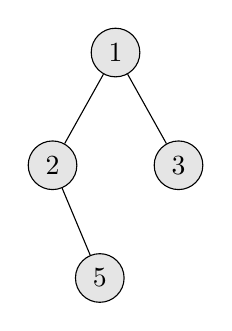
\begin{tikzpicture}
[mynode/.style={draw,circle,minimum size=5mm, fill=gray!20!}]
\node(){};
\node[mynode](A) {1};
\node[mynode](B)[below=8mm of A, xshift=-8mm] {2};
\node[mynode](C)[below=8mm of A, xshift=8mm] {3};
\node[mynode](D)[below=8mm of B, xshift=6mm] {5};
\draw (A) -- (B);
\draw (A) -- (C);
\draw (B) -- (D);
\end{tikzpicture}
\end{figure}
\textbf{Output}: $[1\longrightarrow 2 \longrightarrow 5, 1\longrightarrow 3]$
\\
\textbf{Explanation}: All root-to-leaf paths are: $1\longrightarrow 2\longrightarrow 5$, $1\longrightarrow 3$
\end{flushleft}
\subsection{Depth First Search}
很简单的递归,当遇到leaf node时,就将生成的路径string加入到最终结果中即可。
\setcounter{lstlisting}{0}
\begin{lstlisting}[style=customc, caption={Depth First Search}]
vector<string> binaryTreePaths( TreeNode* root )
{
    vector<string> ans;
    dfs( root, "", ans );

    return ans;
}

void dfs( TreeNode* node, string cur_path, vector<string>& paths )
{
    if( !node )
    {
        return;
    }

    cur_path += to_string( node->val );
    cur_path += "->";

    if( !node->left && !node->right )
    {
        //remove "->"
        cur_path.pop_back();
        cur_path.pop_back();

        paths.emplace_back( cur_path );
        return;
    }

    dfs( node->left, cur_path, paths );
    dfs( node->right, cur_path, paths );
}
\end{lstlisting}
\section{258 --- Add Digits}
Given a non-negative integer $n$, repeatedly add all its digits until the result has only one digit.
\paragraph{Example:}
\begin{flushleft}
\textbf{Input}: 38
\\
\textbf{Output}: 2
\\ 
\textbf{Explanation}: 
\\
The process is like: $3 + 8 = 11$, $1 + 1 = 2$. Since 2 has only one digit, return it.
\end{flushleft}
\paragraph{Follow up:}
\begin{itemize}
\item Could you do it without any loop/recursion in O(1) runtime?
\end{itemize}
\subsection{Mathematical Induction}
Starting from 10, the result is 1 to 9 repeatedly. Therefore, the formula is
\[
x=(n-10)\bmod 9 + 1
\]
\section{259 --- 3Sum Smaller}
Given an array of $n$ integers $A$ and a target $T$, find the number of index triplets $i$, $j$, $k$ with $0 \leq i < j < k < n$ that satisfy the condition $A[i] + A[j] + A[k] < T$.
\par
\paragraph{Example:}
\begin{flushleft}
\textbf{Input}: $A = [-2, 0, 1, 3]$, $T = 2$
\\
\textbf{Output}: 2
\\
\textbf{Explanation}:
\\
Because there are two triplets which sums are less than 2: $[-2, 0, 1]$ and $[-2, 0, 3]$
\end{flushleft}
\paragraph{Follow up:}
\begin{itemize}
\item Could you solve it in $O(n^2)$ runtime?
\end{itemize}
\subsection{Two Indexes: Left And Right}
首先对$A$排序,然后遍历$A$,
\begin{itemize}
\item 在当前index $i$,设定$l$和$r$一左一右两个index,其中$l=i+1$,$r=L-1$(L是$A$的长度);
\item 如果$A[i]+A[l]+A[r]<T$,那么$(i, l, l+1),\ ,(i,l,l+2),\ ,\ldots, (i,l,r)$都是符合要求的triplets。总共有$r-(l+1)+1=r-l$个。接着increments  $l$
\item 如果$A[i]+A[l]+A[r]<\geq T$,这时候需要减小右侧的数,因此decrements $r$。
\end{itemize}
\setcounter{algorithm}{0}
\begin{algorithm}[H]
\caption{Left And Right Indexes}
\begin{algorithmic}[1]
\Procedure{ThreeSumSmaller}{$A, L, T$}
\State $\star$ 对$A$从小到大进行排序
\State $\star$ 初始化变量$\delta$为0,用于记录number of triplets
\For{$i:=0$ \textbf{to} $L-2$}
\State $l:=i+1$
\State $r:=L-1$
\While{$l < r$}
\If{$A[i]+A[l]+A[r] < T$}
\algstore{259algo}
\end{algorithmic}
\end{algorithm}
\begin{algorithm}[H]
\begin{algorithmic}[1]
\algrestore{259algo}
\State $\delta\gets\delta + (r-l)$
\State $l\gets l+1$ \Comment Move $l$ rightwards to test next bigger number
\Else
\State $r\gets r-1$  \Comment Move $r$ leftwards to test next smaller number
\EndIf
\EndWhile
\EndFor
\State \Return $\delta$
\EndProcedure
\end{algorithmic}
\end{algorithm} %$
\section{260 --- Single Number III}
Given an array of numbers $A$, in which exactly two elements appear only once and all the other elements appear exactly twice. Find the two elements that appear only once.

\paragraph{Example:}

\begin{flushleft}
\textbf{Input}:  $[1,2,1,3,2,5]$
\\
\textbf{Output}: $[3,5]$
\end{flushleft}

\paragraph{Note:}

\begin{itemize}
\item The order of the result is not important. So in the above example, $[5, 3]$ is also correct.
\item Your algorithm should run in linear runtime complexity. Could you implement it using only constant space complexity?
\end{itemize}
\subsection{Bit Operation}
\begin{itemize}
\item 由于只有两个数出现一次,因此如果将整个数组的数进行XOR,最终结果肯定就是这两个数的XOR结果,其他的重复两次的数的XOR结果是零。
\item 由于这两个数是不同的,因此这两个数会在某些bit位上不同。这个可以根据XOR的结果中那些bit位为1的位置来确定。
\item 假设在第$i$个bit位上,这两个数是不同的,也就是其中一个数的第$i$个bit位是1,另外一个是零。
\item 因此$A$中所有的数字都可以按照第$i$个bit位分成两个group,一个group中所有的数字在第$i$位是0,另外一个group中的所有数字在第$i$位是1。
\item 然后XOR第一个group中的所有数字就能到两个只出现一次的数字中的一个,然后XOR另外一个group就得到了另一个。
\item 所以找到原来XOR整个数组结果中最右边的第一个1,按照这个bit位进行划分group。\setcounter{lstlisting}{0}
\end{itemize}
\begin{lstlisting}[style=customc, caption={XOR}]
vector<int> singleNumber( vector<int>& nums )
{
    //get xor results of all numbers in nums
    int z = 0;

    for( auto n : nums )
    {
        z ^= n;
    }

    //find which bit is 1
    //and create a mask for this bit
    int mask = 1;

    for( int i = 1; i < 32; ++i )
    {
        if( z & mask )
        {
            break;
        }

        mask <<= 1;
    }

    int x = 0;
    int y = 0;

    //use mask to test which number is set on
    //that bit
    for( auto n : nums )
    {
        if( n & mask )
        {
            x ^= n;
        }
        else
        {
            y ^= n;
        }
    }

    return { x, y };
}
\end{lstlisting}

 
%% %03/15/2019
\section{261 --- Graph Valid Tree}
Given $n$ nodes labeled from 0 to $n - 1$ and a list of undirected edges (each edge is a pair of nodes), write a function to check whether these edges make up a valid tree.
\paragraph{Example 1:}
\begin{flushleft}
\textbf{Input}: $n=5$
\begin{figure}[H]
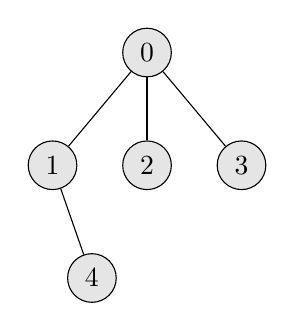
\begin{tikzpicture}
[mynode/.style={draw,circle,minimum size=5mm, fill=gray!20!}]
\node(){};
\node[mynode](A) {0};
\node[mynode](B)[below=8mm of A, xshift=-12mm] {1};
\node[mynode](C)[below=8mm of A] {2};
\node[mynode](D)[below=8mm of A, xshift=12mm] {3};
\node[mynode](E)[below=8mm of B, xshift=5mm] {4};
\draw (A) -- (B);
\draw (A) -- (C);
\draw (A) -- (D);
\draw (B) -- (E);
\end{tikzpicture}
\end{figure}
\textbf{Output}: \texttt{true}
\end{flushleft}

\paragraph{Example 2:}
\begin{flushleft}
\textbf{Input}: $n=5$
\begin{figure}[H]
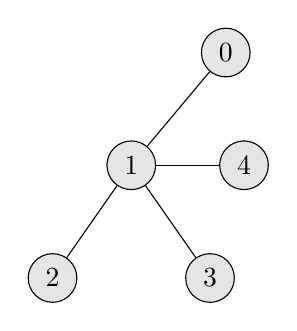
\begin{tikzpicture}
[mynode/.style={draw,circle,minimum size=5mm, fill=gray!20!}]
\node(){};
\node[mynode](A) {0};
\node[mynode](B)[below=8mm of A, xshift=-12mm] {1};
\node[mynode](C)[right=8mm of B] {4};
\node[mynode](D)[below=8mm of B, xshift=-10mm] {2};
\node[mynode](E)[below=8mm of B, xshift=10mm] {3};
\draw (A) -- (B);
\draw (B) -- (C);
\draw (B) -- (D);
\draw (B) -- (E);
\end{tikzpicture}
\end{figure}
\textbf{Output}: \texttt{false}
\end{flushleft}
\paragraph{Hint:}
\begin{itemize}
\item Given $n = 5$ and a graph as below:
\begin{figure}[H]
\centering
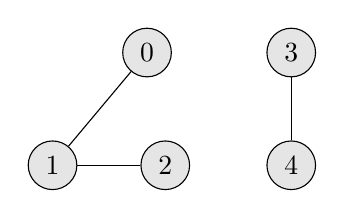
\begin{tikzpicture}
[mynode/.style={draw,circle,minimum size=5mm, fill=gray!20!}]
\node(){};
\node[mynode](A) {0};
\node[mynode](B)[below=8mm of A, xshift=-12mm] {1};
\node[mynode](C)[right=8mm of B] {2};
\node[mynode](D)[right=12mm of A] {3};
\node[mynode](E)[below=8mm of D] {4};
\draw (A) -- (B);
\draw (B) -- (C);
\draw (D) -- (E);
\end{tikzpicture}
\end{figure}
what should your return? Is this case a valid tree?
\item According to the definition of tree on Wikipedia: 
\begin{quote}
a tree is an undirected graph in which any two vertices are connected by exactly one path. 
\end{quote}
In other words, any connected graph without simple cycles is a tree.
\end{itemize}

\paragraph{Note:}
\begin{itemize}
\item you can assume that no duplicate edges will appear in edges. Since all edges are undirected, $[0, 1]$ is the same as $[1, 0]$ and thus will not appear together in edges.
\end{itemize}
\subsection{Depth First Search}
按照定义,Tree其实就是没有cycle的undirected graph。
\begin{itemize}
\item 由于是undirected,因此从edges建立邻接表时,两端节点就要建立邻接表。
\item 然后从第一个节点开始进行深度搜索,用一个颜色标注与其相邻的所有节点。
\item 如果在深度搜索过程中发现某个不是搜索开始的节点已经被标注了相同的颜色,就表示存在cycle。
\end{itemize}
\setcounter{lstlisting}{0}
\begin{lstlisting}[style=customc, caption={DFS}]
bool validTree( int n, vector<pair<int, int>>& edges )
{
    //graph based on adjacent nodes
    vector<vector<int>> g( n, vector<int>() );
    //colors
    vector<int> colors( n, false );

    //create g from edges
    //This is a undirected graph so
    //we have to do for both sides
    for( const auto& e : edges )
    {
        g[e.first].push_back( e.second );
        g[e.second].push_back( e.first );
    }

    if( !dfs( g, v, 0, -1 ) )
    {
        //There exits a cycle
        return false;
    }

    for( int color  : colors )
    {
        //The graph is disjointed
        if( color == 0 )
        {
            return false;
        }
    }
    return true;
}
bool dfs( int start, int parent, vector<vector<int>> &g, vector<int> &colors )
{
    if( colors[start] == 1 )
    {
        //We have visited start before
        //so this is a cycle
        return false;
    }

    //set start node's color to 1
    colors[start] = 1;

    for( int next : g[start] )
    {
        //only check non-parent nodes
        if( next != parent )
        {
            if( !dfs( next, start, g, v ) )
            {
                return false;
            }
        }
    }
    return true;
}

\end{lstlisting}
\subsection{Breath First Search}
\begin{itemize}
\item 需要用queue来辅助遍历,
\item 用一个hash set来记录遍历到的节点。
\item 从节点0开始,将0加入到q中,然后加入到hash set里。开始处理queue。
\item 如果遍历到一个节点,在set中没有,则加入set,如果已经存在,则返回\texttt{false}。
\item 另外在遍历节点$i$的邻接链表的时候,与$i$相连的node在处理完后要把$i$从其邻接表中删除,这样在以后的递归中,如果没有cycle,就不会再返回处理$i$了。
\end{itemize}
\begin{lstlisting}[style=customc, caption={BFS}]
bool validTree( int n, vector<pair<int, int>>& edges )
{
    vector<unordered_set<int>> g( n );

    unordered_set<int> colors;

    //build g from edges
    for( const auto& e : edges )
    {
        g[e.first].insert( e.second );
        g[e.second].insert( e.first );
    }

    queue<int> q;
    //add 0 to queue
    q.push( 0 );
    //color 0
    colors.insert( 0 );

    while( !q.empty() )
    {
        int node = q.front();
        q.pop();

        for( int next : g[node] )
        {
            //There is a cycle
            if( colors.find( next ) != colors.end() )
            {
                return false;
            }

            colors.insert( next );
            q.push( next );

            auto it = g[next].find( node );

            if( it != g[next].end() )
            {
                //remove node from next's adjacent node list
                //to avoid repeat searching
                g[next].erase( it );
            }
        }

    }

    int nodes = static_cast< int >( colors.size() );

    //only when we color all nodes
    //otherwise the graph is disjointed
    return nodes == n;

}
\end{lstlisting}
\subsection{Union}
\begin{itemize}
\item 初始化一个size为$n$的parents数组,其中$\texttt{parents}[i]=i$,即每个节点的parent就是其自身
\item 遍历edges,分别查找edges两边的node的parent,如果发现这两个node的parent相同,表明存在cycle,直接返回\texttt{false}。
\item 如果不相同,将其中一个node的parent设为另外一个node。
\item 最后检查edge的个数是不是$n-1$.
\end{itemize}
\begin{lstlisting}[style=customc, caption={Union Find}]
bool validTree( int n, vector<vector<int>>& edges )
{
    vector<int> parents( n, -1 );
    for( int i = 0; i < n; ++i )
    {
        parents[i] = i;
    }
    vector<int> ranks( n, 1 );
    for( const auto& edge : edges )
    {
        int px = find( edge[0], parents );
        int py = find( edge[1], parents );
        if( px == py )
        {
            //there exists a circle
            return false;
        }
        set_union( px, py, parents, ranks );
    }
    //any two nodes of a tree only one edge connected
    return ( int )( edges.size() ) == n - 1;
}
//find parent
int find( int x, vector<int>& parents )
{
    while( x != parents[x] )
    {
        x = parents[x];
    }
    return x;
}
//union two nodes
void set_union( int x, int y, vector<int>& parents, vector<int>& ranks )
{
    if( ranks[x] > ranks[y] )
    {
        swap( x, y );
    }
    else if( ranks[x] == ranks[y] )
    {
        ranks[x]++;
    }
    parents[y] = x;
}
\end{lstlisting}

\paragraph{Similar Questions}
\begin{itemize}
\item \textbf{207. Course Schedule}
\item \textbf{323. Number of Connected Components in an Undirected Graph}
\end{itemize} %$
%% %262 is a SQL problem
\section{263 -- Ugly Number}
Write a program to check whether a given number is an ugly number.
\par
Ugly numbers are positive numbers whose prime factors only include 2, 3, 5.

\paragraph{Example 1:}

\begin{flushleft}
\textbf{Input}: 6
\\
\textbf{Output}: \texttt{true}
\\
\textbf{Explanation}: $6 = 2 \times 3$
\end{flushleft}


\paragraph{Example 2:}

\begin{flushleft}
\textbf{Input}: 8
\\
\textbf{Output}: \texttt{true}
\\
\textbf{Explanation}: $8 = 2 \times 2 \times 2$
\end{flushleft}

\paragraph{Example 3:}

\begin{flushleft}
\textbf{Input}: 14
\\
\textbf{Output}: \texttt{false} 
\\
\textbf{Explanation}: 
\\
14 is not ugly since it includes another prime factor 7.
\end{flushleft}

\paragraph{Note:}
\begin{itemize}
\item 1 is typically treated as an ugly number.
\item Input is within the 32-bit signed integer range: $[−2^{31},  2^{31} − 1]$.
\end{itemize}
\subsection{Prime Factors}
根据定义,用$n$除以2,3,5一直到不能被这三个数整除。看最后$n$是不是为1。
\setcounter{lstlisting}{0}
\begin{lstlisting}[style=customc, caption={Divide}]
bool isUgly( int num )
{
    while( num >= 2 )
    {
        if( ( num % 2 ) == 0 )
        {
            num /= 2;
        }
        else if( ( num % 3 ) == 0 )
        {
            num /= 3;
        }
        else if( ( num % 5 ) == 0 )
        {
            num /= 5;
        }
        else
        {
            return false;
        }
    }
    return num == 1;
}
\end{lstlisting}

\paragraph{Related Problems}
\begin{itemize}
\item \textbf{279. Perfect Squares}

\end{itemize}
\section{264 --- Ugly Number II}
Write a program to find the $n$-th ugly number.
\par
Ugly numbers are positive numbers whose prime factors only include 2, 3, 5. 

\paragraph{Example:}

\begin{flushleft}
\textbf{Input}: $n = 10$
\\
\textbf{Output}: 12
\\
\textbf{Explanation}: 1, 2, 3, 4, 5, 6, 8, 9, 10, 12 is the sequence of the first 10 ugly numbers.
\end{flushleft}

\paragraph{Note:}  

\begin{itemize}
\item 1 is typically treated as an ugly number.
\item $n$ does not exceed 1690.
\end{itemize}
\subsection{Dynamic Programming}
\begin{itemize}
\item 设定3个计数器$x$,$y$和$z$。分别对应factor 2,3和5。
\item maintain一个size为$n$的DP数组$A$
\item 从第一个ugly number 1开始,$A[0]=1$。下一个数就是$A[0]\times 2$,$A[0]\times 3$和$A[0]\times5$中的最小值,结果是2,因此increment对应2的计数器$x$。所以$A[1]=2$
\item 接下来 $A[2] = \min(A[1]\times2, A[0]\times 3, A[0]\times 5)$。显然是$A[0]\times 3$最小,因此increment对应3的计数器$y$。
\item 以此类推,如果遇到相同的情况,比如6,那么对应的2和3的计数器都要increment。
\end{itemize}


\setcounter{lstlisting}{0}
\begin{lstlisting}[style=customc, caption={Dynamic Programming}]
int nthUglyNumber( int n )
{
    vector<int> A( n, 0 );
    A[0] = 1;
    int id2 = 0;
    int id3 = 0;
    int id5 = 0;
    for( int i = 1; i < n; ++i )
    {
        //find next ugly number
        int n2 = A[id2] * 2;
        int n3 = A[id3] * 3;
        int n5 = A[id5] * 5;
        A[i] = ( min )( n2, n3 );
        A[i] = ( min )( A[i], n5 );
        //check index increment for 2, 3, 5
        //we should check all 3 numbers
        //so no "else if" here
        if( A[i] == n2 )
        {
            ++id2;
        }
        if( A[i] == n3 )
        {
            ++id3;
        }
        if( A[i] == n5 )
        {
            ++id5;
        }
    }
    return A.back();
}
\end{lstlisting}

\paragraph{Related Problems}
\begin{itemize}
\item \textbf{279. Perfect Squares}
\item \textbf{313. Super Ugly Number}
\item \textbf{1201. Ugly Number III}
\end{itemize}
\section{265 --- Paint House II}
There are a row of $n$ houses, each house can be painted with one of the $k$ colors. The cost of painting each house with a certain color is different. You have to paint all the houses such that no two adjacent houses have the same color.
\par
The cost of painting each house with a certain color is represented by a $n \times k$ cost matrix $C$. For example, $C[0][0]$ is the cost of painting house 0 with color 0; $C[1][2]$is the cost of painting house 1 with color 2, and so on. Find the minimum cost to paint all houses.

\paragraph{Note:}
\begin{itemize}
\item All costs are positive integers.
\end{itemize}

\paragraph{Follow up:}
\begin{itemize}
\item Could you solve it in $O(nk)$ runtime?
\end{itemize}
\subsection{Dynamic Programming}
这道题是之前Paint House的拓展,如果用之前的解法,那么对应的时间复杂度将是$O(n\times k\times k)$。
\begin{itemize}
\item 用$a$和$b$分别代表当前第$i-1$个house的minimum cost和second minimum cost。
\item 用$x$和$y$来代表$a$和$b$对应的颜色。
\item 如果第$i$个house的颜色和$x$相同,就用$y$对应的cost也就是$b$进行计算。否则就用$x$对应的cost即$a$。
\item 由于需要更新$a$和$b$,因此当找到比$a$更小的值时,要先把当前的$a$赋给$b$。这样才能保证更新后仍然能够得到正确的$b$。
\end{itemize}

\setcounter{lstlisting}{0}
\begin{lstlisting}[style=customc, caption={Dynamic Programming}]
int minCostII( vector<vector<int>>& costs )
{
    //global minimum
    int min1 = 0;
    //second minimum
    int min2 = 0;
    //the color selected can get global minimum
    int color = -1;
    for( const auto& C : costs )
    {
        //latest global minimum
        int x = INT_MAX;
        //latest second global minimum
        int y = x;
        //color index
        int i = 0;
        //selected color that can get current global minimum
        int paint = -1;
        for( int cost : C )
        {
            //if use color in last house, we cannot
            //use <color>, so add min2
            cost += ( i == color ) ? min2 : min1;
            //update global and second global minimum
            if( cost <= x )
            {
                y = x;
                x = cost;
                paint = i;
            }
            else if( cost < y )
            {
                y = cost;
            }
            ++i;
        }
        //update global
        min1 = x;
        min2 = y;
        color = paint;
    }
    return min1;
}
\end{lstlisting}
\section{266 --- Palindrome Permutation}
Given a string $s$, determine if a permutation of the string could form a palindrome.
\par
For example,
\par
\texttt{code}: \texttt{false}
\par
\texttt{aab}: \texttt{true}
\par
\texttt{carerac}: \texttt{true}

\paragraph{Hint:}

\begin{itemize}
\item Consider the palindromes of odd vs even length. What difference do you notice?
\item Count the frequency of each character.
\item If each character occurs even number of times, then it must be a palindrome. How about character which occurs odd number of times?
\end{itemize}
\subsection{Hash Table}
用一个数组记录每个字母对应的出现次数,然后统计出现次数为奇数的字母的个数,两种情况下是palindrome
\begin{itemize}
\item 没有出现次数为奇数的字母
\item 字符串长度为奇数,且只有一个出现次数为奇数的字母
\end{itemize} %$
\section{267 --- Palindrome Permutation II}
Given a string $s$, return all the palindromic permutations (without duplicates) of it. Return an empty list if no palindromic permutation could be form.
\paragraph{Example 1:}
\begin{flushleft}
\textbf{Input}: $s=\texttt{aabb}$
\\
\textbf{Output}: (\texttt{abba}, \texttt{baab})
\end{flushleft}

\paragraph{Example 2:}
\begin{flushleft}
\textbf{Input}: $s=\texttt{abc}$
\\
\textbf{Output}: $\emptyset$
\end{flushleft}

\paragraph{Hint:}
\begin{itemize}
\item If a palindromic permutation exists, we just need to generate the first half of the string.
\item To generate all distinct permutations of a (half of) string, use a similar approach from: \textbf{47 --- Permutations II} or \textbf{31 --- Next Permutation}.
\end{itemize}
\subsection{Next Permutation}
按照题目的提示,
\begin{itemize}
\item 判断$s$是否可以生成palindrome permutation。
\item 根据string中相同字符的出现次数,取一半构成一个base string。如果长度是odd,就把出现奇数次的字符放在生成的字符串中间位置。
\item 为了避免重复的memory操作,采用copy 字符串的方式。把base copy到生成字符串的左半边,然后reverse copy到生成字符串的右半边。
\item 检查生成的字符串是否在hash set中存在,如果存在,就中断循环。
\item 用next permuatation方法生成下一个base。
\end{itemize}
\setcounter{lstlisting}{0}
\begin{lstlisting}[style=customc, caption={Next Permutation}]
vector<string> generatePalindromes( string s )
{
    unordered_map<char, int> m;

    for( auto c : s )
    {
        auto it = m.find( c );

        if( it == m.end() )
        {
            m.emplace( c, 1 );
        }
        else
        {
            ++it->second;
        }
    }

    int odd_counts = 0;
    char odd_char = 0;

    string base;
    base.reserve( s.size() );

    //generate base i.e. half string for
    //permutation string generation
    for( const auto& p : m )
    {
        int count = p.second;

        if( count & 1 )
        {
            ++odd_counts ;
            odd_char = p.first;
        }
        base.append( count / 2, p.first );
    }


    //Check if s can form palindrome permutation
    if( s.size() & 1 )
    {
        if( odd_counts != 1 )
        {
            return {};
        }
    }
    else
    {
        if( odd_counts > 0 )
        {
            return {};
        }
    }

    unordered_set<string> ss;

    auto next = s;


    size_t righthalf_start = next.size() / 2;
    if( odd_counts != 0 )
    {
        //we set middle character as the odd count's char
        next[righthalf_start] = odd_char;
        ++righthalf_start;
    }

    while( true )
    {
        //use copy to avoid large amount of memory operation
        copy( base.begin(), base.end(), next.begin() );

        size_t start = righthalf_start;

        for( size_t i = 0; i < base.size(); ++i )
        {
            auto j = base.size() - i - 1;
            next[start] = base[j];
            ++start;
        }

        if( ss.find( next ) != ss.end() )
        {
            break;
        }

        ss.emplace( next );


        next_permutation( base );
    }

    return { ss.begin(), ss.end() };
}

//next permutation method
void next_permutation( string& s )
{
    auto L = s.size();

    auto x = L;

    for( size_t i = L - 1; i >= 1; --i )
    {
        if( s[i] > s[i - 1] )
        {
            x = i;
            break;
        }
    }

    if( x == L )
    {
        reverse( s.begin(), s.end() );
        return;
    }

    auto y = x;

    for( size_t j = x; j < L; ++j )
    {
        if( s[j] <= s[x - 1] )
        {
            break;
        }

        y = j;
    }

    swap( s[y], s[x - 1] );

    reverse( s.begin() + x, s.end() );
}

\end{lstlisting} %$
\section{268. Missing Number}
Given an array $A$ containing $n$ distinct numbers taken from $0, 1, 2, \ldots, n$, find the one that is missing from the array.

\paragraph{Example 1:}

\begin{flushleft}
\textbf{Input}: $[3,0,1]$
\\
\textbf{Output}: 2
\end{flushleft}

\paragraph{Example 2:}

\begin{flushleft}
\textbf{Input}: $[9,6,4,2,3,5,7,0,1]$
\\
\textbf{Output}: 8
\end{flushleft}

\paragraph{Note:}
\begin{itemize}
\item Your algorithm should run in linear runtime complexity. \item Could you implement it using only constant extra space complexity?
\end{itemize}
\subsection{Mathematical Induction}
先求出整个数组的和,然后用$(L+1)\times L/2$得到$0,1,\ldots,L$的和,这两个之差即为missing number
\subsection{Bit Manipulation}
由于$A$中只包含了$n$个数,因此index的范围是从$0$到$n-1$,因此将每个index和其对应的数进行XOR,然后再计算整体的XOR,由于重复的数的XOR结果为零,那个missing number就是最终的XOR结果。
\setcounter{lstlisting}{0}
\begin{lstlisting}[style=customc, caption={Bit Manipulation}]
int missingNumber( vector<int>& nums )
{
    int ans = 0;
    for( int i = 0; i < nums.size(); ++i )
    {
        ans ^= ( i + 1 ) ^ nums[i];
    }
    return ans;
}
\end{lstlisting}
\section{269 --- Alien Dictionary}
There is a new alien language which uses the latin alphabet. However, the order among letters are unknown to you. You receive a list of non-empty words $W$ from the dictionary, where words are sorted lexicographically by the rules of this new language. Derive the order of letters in this language.

\paragraph{Example 1:}

\begin{flushleft}
\textbf{Input}
\begin{table}[H]
\begin{tabular}{l}
\texttt{wrt}  \\
\texttt{wrf}  \\
\texttt{er}   \\
\texttt{ett}  \\
\texttt{rftt}
\end{tabular}
\end{table}
\textbf{Output}: \texttt{wertf}
\end{flushleft}

\paragraph{Example 2:}

\begin{flushleft}
\textbf{Input}:
\begin{table}[H]
\begin{tabular}{l}
\texttt{z}  \\
\texttt{x} 
\end{tabular}
\end{table}
\textbf{Output}: \texttt{zx}
\end{flushleft}

\paragraph{Example 3:}

\begin{flushleft}
\textbf{Input}:
\begin{table}[H]
\begin{tabular}{l}
\texttt{z}  \\
\texttt{x} \\
\texttt{z} 
\end{tabular}
\end{table}
\textbf{Output}: $\emptyset$
\\
\textbf{Explanation}: The order is invalid, so return  $\emptyset$.
\end{flushleft}

\paragraph{Note:}

\begin{itemize}
\item You may assume all letters are in lowercase.
\item You may assume that if a is a prefix of b, then a must appear before b in the given dictionary.
\item If the order is invalid, return an empty string.
\item There may be multiple valid order of letters, return any one of them is fine.
\end{itemize}
\subsection{BFS}
这其实是build a directed graph, calculate each node's in-degree and output them according to in-degree.
\begin{itemize}
\item 构建出相邻的word在相同的位置上的letter形成的edges所构成的graph。
\item 同时用一个hash set保存所有words中的letters。
\item 边界情况:例如\texttt{baac}出现在\texttt{baa}之前,这种情况下不是valid order。
\end{itemize}
\setcounter{algorithm}{0}
\begin{algorithm}[H]
\caption{BFS}
\begin{algorithmic}[1]
\Procedure{AlienOrder}{$W, L$}
\State $\star$ 初始化一个hash set $C$
\State $\ast$ 构建出directed grap $G$
\For{$i:=0$ \textbf{to} $L-1$}
\State $\star$ All all characters of $W[i]$ to $C$
\State $\star$ 得到$W[i]$和$W[i+1]$的最小length $\ell$
\If{$W[i][0\ldots\ell-1]$ is equal to $W[i+1][0\ldots\ell-1]$ }
\If{$W[i]$'s length is larger than $W[i+1]$'s length}
\State \Return $\emptyset$ \Comment 这是invalid order
\EndIf
\EndIf
\State $\star$ Add edge ($W[i][j], W[i][j]$) to $g$ for the first $j$ where $W[i][j]\neq W[i+1][j]$: 
\State $\star$ while iterating $j$ from 0 to $\ell-1$
\EndFor
\State $\star$ Add all characters of $W[L-1]$ to $C$ \Comment 上述循环没有处理$W[L-1]$
\algstore{269algo}
\end{algorithmic}
\end{algorithm}
\begin{algorithm}[H]
\begin{algorithmic}[1]
\algrestore{269algo}
\State $\star$ 遍历$g$的每个edge,计算其中每个edge的终止点的in-degree。
\State $\star$ 将$g$所有in-degree为零的节点加入queue $q$中。同时输出到结果序列$S$中。
\While{$q\neq\emptyset$}
\State $\star$ 弹出$q$的\texttt{front} $x$
\State $\star$ 在$g$中找到所有与$x$的相连的nodes,decrements their in-degrees
\State $\star$ 如果某个node的in-degree变为零, push it into $q$.同时输出该节点到结果序列$S$中。
\EndWhile
\State $\star$ 检查$S$中的节点个数是否与$C$中的节点个数相等: 
\State $\star$ 如果不相等,说明$g$中存在cycle,显然是invalid order,因此返回空序列。
\State $\star$ 如果相等,则返回$S$
\EndProcedure
\end{algorithmic}
\end{algorithm}
\setcounter{lstlisting}{0}
\begin{lstlisting}[style=customc, caption={BFS}]
string alienOrder( vector<string>& words )
{
    unordered_map<char, unordered_set<char>> g;

    unordered_set<char> chs;

    auto L = static_cast< int >( words.size() );

    for( int i = 0; i < L - 1; ++i )
    {
        auto& w1 = words[i];
        auto& w2 = words[i + 1];

        chs.insert( w1.begin(), w1.end() );

        auto len = ( min )( w1.size(), w2.size() );
        auto k = 0;

        for( k = 0; k < len; ++k )
        {
            if( w1[k] != w2[k] )
            {
                auto it = g.find( w1[k] );

                if( it == g.end() )
                {
                    g.emplace( w1[k], initializer_list<char> { w2[k] } );
                }
                else
                {
                    it->second.emplace( w2[k] );
                }

                break;
            }
        }

        //Invalid Order
        if( ( k == len ) && ( w1.size() > w2.size() ) )
        {
            return "";
        }
    }

    // add final word's characters into the
    chs.insert( words.back().begin(), words.back().end() );

    vector<int> v_degIn( 26, 0 );

    for( const auto& p : g )
    {
        for( auto c : p.second )
        {
            v_degIn[c - 'a']++;
        }
    }

    queue<char> q;

    string ans = "";

    for( auto c : chs )
    {
        if( v_degIn[c - 'a'] == 0 )
        {
            // add in-degree=0 nodes
            // into the queue
            q.push( c );
            ans.push_back( c );
        }
    }

    while( !q.empty() )
    {
        auto c = q.front();
        q.pop();

        for( auto next : g[c] )
        {
            v_degIn[next - 'a']--;

            if( v_degIn[next - 'a'] == 0 )
            {
                q.push( next );
                ans.push_back( next );
            }
        }
    }

    if( ans.size() == g.size() )
    {
        return ans;
    }

    //There exists a cycle
    return "";

}
\end{lstlisting}
\subsection{DFS}
如果用Depth First Search,需要改变$g$的存储结构: 用一个Boolean二维数组。如果$g[i][j]=\texttt{true}$,就表示有directed edge between $i$ and $j$。
\par
另外采用这种结构就不需要用额外的hash set去存储所有words中的letter,只需要将$g[i][i]=\texttt{true}$。
\par
DFS需要对已经访问的节点进行mark,但可以从任何一个node开始进行深度搜索。由于题目中所有的words中只包含了lowercase letter,因此可以逐个递归粗粒26个lowercase letter。
\par
在递归中
\begin{itemize}
\item 检测该字符是否包含在words中
\item 访问从该字符出发的与其相连的其他字符。检测这些字符有没有被访问过,如果访问过,表明存在cycle。输出invalid order即空序列。
\item 然后继续从这些字符进行深度搜索。任何一个深度搜索返回invalid order都直接输出空序列。
\item 如果这些字符都是valid order,将当前字符标注为已访问。同时将其标注为不在words中的letter。
\item 由于加入letter到输出序列是在每次深度搜索完成后,因此最后产生的序列其实是倒序的,返回时需要将这个序列进行reverse。
\end{itemize}
根据上述递归过程,在字典序排序后面的字符会比前面的更早处理。如果最开始进行DFS的letter是字典序排序最前面的,那么经过从这个letter开始的深度搜索一次就完成了字典序列的创建。
\setcounter{lstlisting}{0}
\begin{lstlisting}[style=customc, caption={DFS}]
string alienOrder( vector<string>& words )
{
    vector<vector<unsigned char>> g( 26, vector<unsigned char> ( 26, 0 ) );

    auto L = static_cast< int >( words.size() );

    //A helper function to add letters from
    //a string to g
    auto add_chars = [&g]( const string & w )
    {
        for( auto c : w )
        {
            g[c - 'a'][c - 'a'] = 1;
        }
    };

    for( int i = 0; i < L - 1; ++i )
    {
        auto &w1 = words[i];
        auto &w2 = words[i + 1];

        add_chars( w1 );

        auto l = ( min )( w1.size(), w2.size() );

        size_t k = 0;

        for( ; k < l; ++k )
        {
            if( w1[k] != w2[k] )
            {
                g[w1[k] - 'a'][w2[k] - 'a'] = 1;
                break;
            }
        }

        //this is invalid order
        if( ( k == l ) && ( w1.size() > w2.size() ) )
        {
            return "";
        }
    }

	//The last word also needs to be added
    add_chars( words.back() );

    vector<unsigned char> seen( 26, 0 );

    string ans;

    //test each letter by DFS
    for( char c = 'a'; c <= 'z'; ++c )
    {
        int i = c - 'a';
        if( !dfs( i, g, seen, ans ) )
        {
            return "";
        }
    }

    return string( ans.rbegin(), ans.rend() );
}

bool dfs( int x, vector<vector<unsigned char>>&g, vector<unsigned char>& seen, string &ans )
{
    if( g[x][x] == 0 )
    {
        return true;
    }
    seen[x] = 1;

    for( int i = 0; i < 26; ++i )
    {
        if( ( i == x ) || ( g[x][i] == 0 ) )
        {
            continue;
        }

        if( seen[i] == 1 )
        {
            return false;
        }

        if( !dfs( i, g, seen, ans ) )
        {
            return false;
        }
    }

    //mark this letter as
    //unseen and not included in words
    //to make sure no repeat
    seen[x] = 0;
    g[x][x] = 0;

    ans.push_back( x + 'a' );

    return true;
}
\end{lstlisting} %$
\section{270 --- Closest Binary Search Tree Value}
Given a non-empty binary search tree and a target value $T$, find the value in the BST that is closest to the target.

\paragraph{Note:}

\begin{itemize}
\item Given target value is a floating point.
\item You are guaranteed to have only one unique value in the BST that is closest to the target.
\end{itemize}
\subsection{BST}
由于是比较浮点值,因此用当前节点的值和目标值的差的绝对值作为close的判定依据。
\setcounter{lstlisting}{0}
\begin{lstlisting}[style=customc,caption={BST}]
int closestValue( TreeNode* root, double target )
{
    int ans = root->val;
    auto node = root;

    while( node )
    {
        //compare the abs value
        if( abs( ans - target ) >= abs( node->val - target ) )
        {
            ans = node->val;
        }
        node = target < node->val ? node->left : node->right;
    }
    return ans;
}
\end{lstlisting}

\paragraph{Related Problems}
\begin{itemize}
\item \textbf{222. Count Complete Tree Nodes}
\item \textbf{272. Closest Binary Search Tree Value II}
\item \textbf{700. Search in a Binary Search Tree}
\end{itemize} %$
\section{271 --- Encode and Decode Strings}
Design an algorithm to encode a list of strings $A$ to a string $S$. The encoded string is then sent over the network and is decoded back to the original list of strings.
\par
Machine 1 (\textbf{sender}) has the function:

\begin{lstlisting}[style=customc]
string encode(vector<string> strs) {
  // ... your code
  return encoded_string;
}
\end{lstlisting}

Machine 2 (\textbf{receiver}) has the function:

\begin{lstlisting}[style=customc]
vector<string> decode(string s) {
  //... your code
  return strs;
}
\end{lstlisting}
 

So Machine 1 does:

\begin{lstlisting}[style=customc]
string encoded_string = encode(strs);
\end{lstlisting}
 

and Machine 2 does:

\begin{lstlisting}[style=customc]
vector<string> strs2 = decode(encoded_string);
\end{lstlisting}
 

\texttt{strs2} in Machine 2 should be the same as \texttt{strs} in Machine 1.
\par
Implement the \texttt{encode} and \texttt{decode} methods.

\paragraph{Note:}

\begin{itemize}
\item The string may contain any possible characters out of 256 valid \texttt{ascii} characters. Your algorithm should be generalized enough to work on any possible characters.
\item Do not use class member/global/static variables to store states. Your encode and decode algorithms should be stateless.
\item Do not rely on any library method such as \texttt{eval} or \textbf{serialize} methods. You should implement your own encode/decode algorithm.
\end{itemize}
\subsection{Analysis}
\begin{itemize}
\item 如果不涉及到复杂的编码算法设计,这道题其实可以很简单的将每个字符串拼接起来,中间用一个特殊字符进行分开,同时将每个字符串的长度编码转换成字符串加入到输出string中。
\item 由于可能string中可能会包含不属于ASCII的字符,因此特殊字符可以用backslah或者字符串的末尾结束符。
\end{itemize} %$
\section{272 --- Closest Binary Search Tree Value IIe}
Given a non-empty binary search tree and a target value $T$, find $k$ values in the BST that are closest to the target.

\paragraph{Note:}

\begin{itemize}
\item Given target value is a floating point.
\item You may assume $k$ is always valid, that is: $k \leq$ total nodes.
\item You are guaranteed to have only one unique set of $k$ values in the BST that are closest to the target.
\end{itemize}
 
\paragraph{Follow up:}
\begin{itemize}
\item Assume that the BST is balanced, could you solve it in less than $O(n)$ runtime (where $n =$ total nodes)?
\end{itemize}

\paragraph{Hint:}

\begin{enumerate}
\item Consider implement these two helper functions:
\begin{enumerate}
\item \texttt{getPredecessor}($N$), which returns the next smaller node to $N$.
\item \texttt{getSuccessor}($N$), which returns the next larger node to $N$.
\end{enumerate}
\item Try to assume that each node has a parent pointer, it makes the problem much easier.
\item Without parent pointer we just need to keep track of the path from the root to the current node using a stack.
\item You would need two stacks to track the path in finding \textbf{predecessor} and \textbf{successor} node separately.
\end{enumerate}
\subsection{In-order Traverse}
\begin{itemize}
\item In-order traverse on BST得到的是从小到大排序的序列。
\item 在in-order traverse中,如果当前结果序列的size小于$k$,直接把访问的节点的值放入结果序列$A$中。
\item 如果当前结果序列的size等于$k$了,则将当前访问的节点值与当前结果序列$A$的第一个值$A[0]$按照与$T$的差的绝对值进行比较。如果当前节点值与$T$的差的绝对值更小,说明当前节点值与$T$更接近,将$A[0]$从$A$中去除,将当前节点值加到$A$的末尾。
\item 比较$A[0]$而不是$A$其他的元素,是因为$A[0]$是$A$中最小的number。如果当前节点值比$A[0]$更靠近$T$,那么由于当前节点值比$A$中所有的number都要大,所以除了$A[0]$外的其他number肯定都要比$A[0]$更接近$T$。而我们需要得到$k$个更接近$T$的值,因此只需要移除掉$A[0]$。
\item 如果当前节点值与$T$的差的绝对值比$A[0]$的更大,这时候就不用再继续遍历了,因为后面的节点值与$T$的差的绝对值更大。
\end{itemize}
\setcounter{algorithm}{0}
\begin{algorithm}[H]
\caption{In-order Traverse}
\begin{algorithmic}[1]
\Procedure{ClosestKValues}{$R, T, k$}
\State $\star$ Create the result array $A$
\State \Call{InOrder}{$S=R, T, A, K=k$} \Comment Call function \texttt{InOrder}
\State \Return $A$
\EndProcedure
\end{algorithmic}
\end{algorithm}
Function \texttt{InOrder} traverse the BST tree start from node $S$.

\begin{algorithm}[H]
\caption{Helper Function For In-order Traverse}
\begin{algorithmic}[1]
\Procedure{InOrder}{$S, T, A, K$}
\If{$S$ is null node}
\State \Return
\EndIf
\State $\star$ Call \texttt{InOrder} on left subtree of $S$
\If{size of $A$ is less than $K$}
\State $\star$ 将$S$的节点值加到$A$的末尾
\Else
\If{$S$的节点值与$K$的差的绝对值小于$\lvert K-A[0]\rvert$}
\State $\star$ Remove $A[0]$ from $A$
\State $\star$ 将$S$的节点值加到$A$的末尾
\Else
\State \Return \Comment 后面遍历到的节点值会更偏离$T$
\algstore{272algo}
\end{algorithmic}
\end{algorithm}
\begin{algorithm}[H]
\begin{algorithmic}[1]
\algrestore{272algo}
\EndIf
\EndIf
\State $\star$ Call \texttt{InOrder} on right subtree of $S$
\EndProcedure
\end{algorithmic}
\end{algorithm}
\setcounter{lstlisting}{0}
\begin{lstlisting}[style=customc,caption={In-order Traverse}]
vector<int> closestKValues( TreeNode* root, double target, int k )
{
    vector<int> ans;
    ans.reserve( k );

    auto K = static_cast< size_t >( k );

    inorder( root, target, ans, K );

    return ans;
}

void inorder( TreeNode* node, double T, vector<int>& A, size_t k )
{
    if( !node )
    {
        return;
    }

    inorder( node->left, T, A, k );

    if( A.size() < k )
    {
        A.push_back( node->val );
    }
    else
    {
        auto a0 = static_cast< double >( A[0] );
        auto dv = static_cast< double >( node->val );


        if( abs( a0 - T ) > abs( dv - T ) )
        {
            //node-val is closer to T
            //Remove A[0]
            A.erase( A.begin() );
            //Add node->val
            A.push_back( node->val );
        }
        else
        {
            //We cannot find value that is closer to T
            //from now on
            return;
        }
    }

    inorder( node->right, T, A, k );
}
\end{lstlisting}
\subsection{Based On Hints}
\begin{itemize}
\item Maintian two stacks: $P$ and $S$。
\item At start, 根据BST的特性,将节点值小于$T$的节点push到$P$中,将节点值大于或者等于$T$的节点push到$S$中。
\item 然后循环$k$次,每次都比较$P$和$S$的栈顶node的value哪个更close to $T$。
\item 如果$P$的栈顶node的value更close to $T$,将这个栈顶node的value输出到结果序列$A$中并从$P$中删除该node。接下来借助函数\texttt{getPredecessor}寻找the next smaller node to this node。在BST中,这个next \textbf{smaller} node是该节点的\textbf{左子树的最右节点}如果该节点的左子树存在。在寻找的过程中,把路径上的所有节点都push到$P$中。
\item 如果$S$的栈顶node的value更close to $T$,将这个栈顶node的value输出到结果序列$A$中并从$S$中删除该node。接下来借助函数\texttt{getSuccessor}寻找the next \textbf{larger} node to this node。在BST中,这个next \textbf{larger} node是该节点的\textbf{右子树的最左节点}如果该节点的右子树存在。在寻找的过程中,把路径上的所有节点都push到$S$中。
\end{itemize}
\begin{algorithm}[H]
\caption{Find Next Larger And Next Smaller Node}
\begin{algorithmic}[1]
\Procedure{ClosestKValues}{$R, T, k$}
\State $\star$ Create two stacks $P$ and $S$
\State $\ast$ Push nodes whose values less than $T$ to $P$. Otherwise, push to $S$
\State $x:=R$
\While{$x$ is not null node}
\If{value of $x$ is less than $T$}
\State $\star$ Push $x$ to $P$
\State $\star$ Update $x$ to its left child node
\Else
\State $\star$ Push $x$ to $S$
\State $\star$ Update $x$ to its right child node
\EndIf
\EndWhile
\State $\delta:=0$ \Comment The counter of loops
\State $\star$ Create an array $A$ as the result array
\While{$\delta < k$}
\If{$S$ is empty \textbf{or} top node's value of $P$ is closer to $T$}
\State $\star$ Add $P$'s top node's value to $A$
\State $\star$ Call \texttt{GetPredecessor} to find next smaller nodes to $P$'s top node
\Else
\State $\star$ Add $S$'s top node's value to $A$
\State $\star$ Call \texttt{GetSuccessor} to find next larger nodes to $S$'s top node
\EndIf
\State $\delta\gets\delta+1$ \Comment Increments the counter of loops
\EndWhile
\State \Return $A$
\EndProcedure
\end{algorithmic}
\end{algorithm}
Function \texttt{GetPredecessor}寻找the next smaller node to $P$'s top node。同时把路径上的节点都push到$P$中。
\begin{algorithm}[H]
\caption{Get Next Smaller Node}
\begin{algorithmic}[1]
\Procedure{GetPredecessor}{$P$}
\State $\star$ Set $t$ as $P$'s top node
\State $\star$ Pop $P$'s top node
\If{$t$'s left child node is not null}
\State $\star$ Push $t$'s \textbf{left} child node to $P$
\State $\star$ Update $t$ as its left child node
\While{$t$'s \textbf{right} child node is not null}
\State $\star$ Push $t$'s \textbf{right} child node to $P$
\State $\star$ Update $t$ as its \textbf{right} child node
\EndWhile
\EndIf
\EndProcedure
\end{algorithmic}
\end{algorithm}
Function \texttt{GetSuccessor}寻找the next larger node to $S$'s top node。同时把路径上的节点都push到$S$中。

\begin{algorithm}[H]
\caption{Get Next Larger Node}
\begin{algorithmic}[1]
\Procedure{GetSuccessor}{$S$}
\State $\star$ Set $t$ as $S$'s top node
\State $\star$ Pop $S$'s top node
\If{$t$'s right child node is not null}
\State $\star$ Push $t$'s \textbf{right} child node to $S$
\State $\star$ Update $t$ as its right child node
\While{$t$'s \textbf{left} child node is not null}
\State $\star$ Push $t$'s \textbf{left} child node to $S$
\State $\star$ Update $t$ as its \textbf{left} child node
\EndWhile
\EndIf
\EndProcedure
\end{algorithmic}
\end{algorithm}
\begin{lstlisting}[style=customc, caption={Find Next Larger And Next Smaller Node}]
vector<int> closestKValues( TreeNode* root, double target, int k )
{
    stack<TreeNode*> P;
    stack<TreeNode*> S;

    auto node = root;

    while( node )
    {
        auto dv = static_cast< double >( node->val );

        if( dv < target )
        {
            P.push( node );
            node = node->right;
        }
        else
        {
            S.push( node );
            node = node->left;
        }

    }

    int loops = 0;
    vector<int> ans;
    ans.reserve( k );

    while( loops < k )
    {
        double dp = P.empty() ? 0 : abs( static_cast< double >( P.top()->val ) - target );
        double ds = S.empty() ? 0 : abs( static_cast< double >( S.top()->val ) - target );

        if( S.empty() )
        {
            ans.push_back( P.top()->val );
            getPredecessor( P );
        }
        else if( !P.empty() && ( dp < ds ) )
        {
			//P.top() is closer to T
            ans.push_back( P.top()->val );
            getPredecessor( P );
        }
        else //S is not empty or P is empty or dp >= ds
        {
            ans.push_back( S.top()->val );
            getSuccessor( S );
        }

        ++loops;
    }

    return ans;
}
//Get next smaller node to P.top()
void getPredecessor( stack<TreeNode*>& P )
{
    auto t = P.top();
    P.pop();

    if( t->left )
    {
        P.push( t->left );
        t = t->left;
        while( t->right )
        {
            P.push( t->right );
            t = t->right;
        }
    }
}
//Get next larger node to S.top()
void getSuccessor( stack<TreeNode*>& S )
{
    auto t = S.top();
    S.pop();

    if( t->right )
    {
        S.push( t->right );

        t = t->right;
        while( t->left )
        {
            S.push( t->left );
            t = t->left;
        }

    }
}
\end{lstlisting} %$
\section{273 --- Integer to English Words}
Convert a non-negative integer $n$ to its english words representation. Given input is guaranteed to be less than $2^{31} - 1$.

\paragraph{Example 1:}

\begin{flushleft}
\textbf{Input}: 123
\\
\textbf{Output}: One Hundred Twenty Three
\end{flushleft}

\paragraph{Example 2:}

\begin{flushleft}
\textbf{Input}: 12345
\\
\textbf{Output}: Twelve Thousand Three Hundred Forty Five
\end{flushleft}

\paragraph{Example 3:}

\begin{flushleft}
\textbf{Input}: 1234567
\\
\textbf{Output}: One Million Two Hundred Thirty Four Thousand Five Hundred Sixty Seven
\end{flushleft}

\paragraph{Example 4:}

\begin{flushleft}
\textbf{Input}: 1234567891
\\
\textbf{Output}:
\\
One Billion Two Hundred Thirty Four Million Five Hundred Sixty Seven Thousand Eight Hundred Ninety One
\end{flushleft}
\subsection{Process Each Hundred Segment}
\begin{itemize}
\item 每次将$n$除以1000,余数就是小于1000的数,对这个余数进行处理得到英文的表达式
\item 之后按照商是否大于零,分别加上Thousand,Million和Billion。
\end{itemize}

\setcounter{lstlisting}{0}
\begin{lstlisting}[style=customc,caption={Process Each Segment}]
string numberToWords( int num )
{
    vector<string> v1000 =
    {
        "Thusand", "Million", "Billion"
    };

    vector<string> v1 =
    {
        "",
        "One", "Two", "Three",
        "Four", "Five", "Six",
        "Seven", "Eight", "Nine",
        "Ten", "Eleven", "Twelve",
        "Thirteen", "Fourteen", "Fifteen",
        "Sixteen", "Seventeen", "Eighteen",
        "Nineteen"
    };

    vector<string> v20 =
    {
        "", "",
        "Twenty", "Thirty", "Forty",
        "Fifty", "Sixty",
        "Seventy", "Eighty",
        "Ninety"
    };

    //The sepration between each thousand
    int level = 0;

    int q = num / 1000;
    int r = num - 1000 * q;

    num = q;

    //Process the first hundred segment
    string ans = process_hundred( r, v1, v20 );

    while( num != 0 )
    {

        q = num / 1000;
        r = num - 1000 * q;

        if( r != 0 )
        {
            auto prev = ans;
            ans = process_hundred( r, v1, v20 ) + " " + v1000[level];
            ans.push_back( ' ' );
            ans += prev;
        }

        ++level;
        num = q;
    }

    while( !ans.empty() && ( ans.back() == ' ' ) )
    {
        ans.pop_back();
    }

    return ans.empty() ? "Zero" : ans;
}

//Transform less than 1000 to english word
string process_hundred( int n, vector<string>& v1,  vector<string>& v20 )
{
    if( n < 20 )
    {
        return v1[n];
    }

    if( n < 100 )
    {
        int q = n / 10;
        int r = n - 10 * q;

        if( r == 0 )
        {
            return v20[q];
        }

        return v20[q] + " " + v1[r];
    }

    int q = n / 100;
    int r = n - 100 * q;

    if( r == 0 )
    {
        return v1[q] + " Hundred";
    }

    auto next = process_hundred( r, v1, v20 );
    return  v1[q] + " Hundred " + next;
}
\end{lstlisting}
\section{274 --- H-Index}
Given an array of citations (each citation is a non-negative integer) of a researcher $A$, write a function to compute the researcher's \textbf{h-index}.
\par
According to the definition of \textbf{h-index} on Wikipedia:
\begin{quote}
 A scientist has index $h$ if $h$ of his/her $N$ papers have at least h citations each, and the other $N - h$ papers have no more than $h$ citations each.
\end{quote}

\paragraph{Example:}

\begin{flushleft}
\textbf{Input}: $A = [3,0,6,1,5]$
\\
\textbf{Output}: 3 
\\
\textbf{Explanation}: 
\\
$[3,0,6,1,5]$ means the researcher has 5 papers in total and each of them had received 3, 0, 6, 1, 5 citations respectively. 
\\
Since the researcher has 3 papers with at least 3 citations each and the remaining two with no more than 3 citations each, her \textbf{h-index} is 3.
\end{flushleft}
\paragraph{Note:} 
\begin{itemize}
\item If there are several possible values for $h$, the maximum one is taken as the \textbf{h-index}
\end{itemize}
\subsection{Bucket Sort}
\begin{itemize}
\item 假设有$x$篇论文的引用数都大于或者等于$x$,那么这个$x$就是H-index。
\item 假设$n$是总的论文数,将这些论文放入$n+1$个buckets中,这些bucket的编号从0到$n$。
\item 对于每一篇论文,如果其引用数与bucket的index相等,就将其放入这个bucket中。
\item 对于那些大于$n$引用数的论文,都将其放入编号为$n$的bucket中。
\item 然后从第$n$个bucket开始往前遍历,累加每个bucekt中的论文数量,当发现累加值大于当前bucket的index,那么这个index就是H-index。
\begin{enumerate}
\item 之所以要从$n$往前遍历,是因为题目要求在存在几个可能的H-index的情况下,取最大的。
\end{enumerate}
\end{itemize}

\setcounter{lstlisting}{0}
\begin{lstlisting}[style=customc, caption={Bucket Sort}]
int hIndex( vector<int>& citations )
{
    vector<int> buckets( citations.size() + 1, 0 );

    int L = static_cast< int >( citations.size() );

    for( auto n : citations )
    {
        if( n > L )
        {
            ++buckets.back();
        }
        else
        {
            ++buckets[n];
        }
    }

    int total = 0;
    //iterate from $L$ to 0
    //to get largest H-index
    for( int i = L; i >= 0; --i )
    {
        total += buckets[i];
        if( total >= i )
        {
            //i is the H-index
            return i;
        }
    }

    return 0;

}
\end{lstlisting}
\section{275 --- H-Index II}
Given an array of citations \textbf{sorted in ascending order} (each citation is a non-negative integer) of a researcher, write a function to compute the researcher's h-index.
\par
According to the definition of \textbf{h-index} on Wikipedia:
\begin{quote}
 A scientist has index $h$ if $h$ of his/her $N$ papers have at least h citations each, and the other $N - h$ papers have no more than $h$ citations each.
\end{quote}

\paragraph{Example:}

\begin{flushleft}
\textbf{Input}: $A = [0,1,3,5,6]$
\\
\textbf{Output}: 3 
\\
\textbf{Explanation}: 
\\
$[0,1,3,5,6]$ means the researcher has 5 papers in total and each of them had received 0, 1, 3, 5, 6 citations respectively. 
\\
Since the researcher has 3 papers with \textbf{at least} 3 citations each and the remaining two with \textbf{no more than} 3 citations each, her \textbf{h-index} is 3.
\end{flushleft}
\paragraph{Note:} 
\begin{itemize}
\item If there are several possible values for $h$, the maximum one is taken as the \textbf{h-index}
\end{itemize}

\paragraph{Follow up:}

\begin{itemize}
\item This is a follow up problem to \textbf{274 --- H-Index}, where citations is now guaranteed to be sorted in ascending order.
\item Could you solve it in \textbf{logarithmic} time complexity?
\end{itemize}
\subsection{Binary Search}
\begin{itemize}
\item 由于数组是排序的,因此binary search找到第一个index $i$,使得$A[i]\geq L -i $,其中$L$是$A$的长度。由于$A[i]$到$A[L-1]$有$L-i$个数,因此只要这些数都大于或者等于$L-i$,就找到了符合要求的H-index。
\item 找到$i$后,$L-i$就是H-index。
\item 很显然这就是leftmost binary search
\end{itemize}
\setcounter{lstlisting}{0}
\begin{lstlisting}[style=customc, caption={Leftmost Binary Search}]
int hIndex( vector<int>& citations )
{
    if( citations.empty() )
    {
        return 0;
    }

    int L = static_cast<int>( citations.size() );

    int l = 0;
    int r = L;

    //leftmost binary search
    //find first index i where A[i]>=L-i
    while( l < r )
    {
        int mid = ( l + r ) / 2;
        if( citations[mid] < L - mid )
        {
            l = mid + 1;
        }
        else
        {
            r = mid;
        }
    }

    //L-i is the H-index
    return L - l;
}
\end{lstlisting}
\section{276 --- Paint Fence}
There is a fence with $n$ posts, each post can be painted with one of the $k$ colors.
\par
You have to paint all the posts such that no more than two adjacent fence posts have the same color.
\par
Return the total number of ways you can paint the fence.
\par
\paragraph{Note:}
\begin{itemize}
\item $n$ and $k$ are non-negative integers.
\end{itemize}
\subsection{Dynamic Programming}
\begin{itemize}
\item $n=1$: 那么有$k$个方法,因为有$k$种颜色可以选择。
\item $n=2$: 分两种情况来统计,
\begin{enumerate}
\item 相邻部分没有相同的,这种情况下,第一个post有$k$个颜色可以选择,而第二个post就只能有$k-1$种颜色选择。因此有$k\times (k-1)$个方法。
\item 相邻部分具有相同颜色,这种情况下,两个post都有$k$种颜色可以选择,因此有$k\times k$个方法。
\item 总共有$k\times k+k\times(k-1) = k^2$
\end{enumerate}
\item $n=3$:同样是两种情况,\begin{enumerate}
\item 如果与第二个post颜色相同,那么显然第二个post不能选择和第一个post相同的颜色,因此这种情况下的方法即为第二个post刷与第一个post不同颜色的方法即$k\times(k-1)$。
\item 而如果与第二个post颜色不同,那么第二个post既能够和第一个post具有相同颜色,也可以与第一个post有不相同的颜色,也就是刷第二个post的总的方法即$k^2$在乘以第三个post能够选择的颜色种类即$k-1$,因为只要与第二个post不同颜色就行,与第一个post颜色相同没有关系。
\end{enumerate}
\end{itemize}
综上所述,假设有数组$x$和$y$
\begin{itemize}
\item $x[i]$表示第$i$个post与第$i-1$个post具有相同颜色的方法数
\item $y[i]$表示第$i$个post与第$i-1$个post有不相同颜色的方法数。
\end{itemize}
那么,第$i$个post的方法$F[i]$与第$i-1$个post的方法$F[i-1]$的关系如下
\begin{align*}
F[i-1] &= x[i-1] + y[i-1]\\
x[i] &= y[i-1]\\
y[i] &= F[i-1]\times(k-1)\\
F[i] &= x[i] + y[i]\\
\end{align*}
由于上述递推关系之和$i-1$有关,因此具体代码实现时,可以用两个变量来代表$x[i]$和$y[i]$
\setcounter{algorithm}{0}
\begin{algorithm}[H]
\caption{Dynamic Programming}
\begin{algorithmic}[1]
\Procedure{NumWays}{$n,k$}
\If{$n=0$}
\State \Return 0
\EndIf
\State $\ast$ $n=1$时,只有一个post,所以有$k$个方法
\State $x:=0$
\State $y:=k$
\State $F:=x+y$
\For{$i:=2$ \textbf{to} $n$}
\State $\ast$ $x[i]\gets y[i-1]$ The number ways that $i$th post has same color as $(i-1)$th post
\State $x\gets y$ 
\State $\ast$ $x[i]\gets y[i-1]$ The number ways that $i$th post has different color than $(i-1)$th post
\State $y\gets F\times (k-1)$ 
\State $\ast$ $F[i]\gets x[i]+y[i]$ The total ways that $i$th post can be painted
\State $F\gets x+y$ 
\EndFor
\State \Return $F$
\EndProcedure
\end{algorithmic}
\end{algorithm}
\setcounter{lstlisting}{0}
\begin{lstlisting}[style=customc, caption={Dynamic Programming}]
int numWays( int n, int k )
{
    if( n == 0 )
    {
        return 0;
    }

    int x = 0; //when current post and last post have same colors
    int y = k; //when current post and last post have different colors
    int F = x + y; //The total ways to paint current post

    for( int i = 2; i <= n; ++i )
    {
        x = y; //x[i]=y[i-1]
        y = F * ( k - 1 ); //y[i]=F*(k-1)
        F = x + y; //F[i]=x[i]+y[i]
    }
    return F;
}
\end{lstlisting} %$
\section{277 --- Find the Celebrity}
Suppose you are at a party with $n$ people (labeled from 0 to $n-1$) and among them, there may exist one celebrity. The definition of a celebrity is that all the other $n-1$ people know him/her but he/she does not know any of them.
\par
Now you want to find out who the celebrity is or verify that there is not one. The only thing you are allowed to do is to ask questions like: ``Hi, A. Do you know B?'' to get information of whether $A$ knows $B$. You need to find out the celebrity (or verify there is not one) by asking as few questions as possible (in the asymptotic sense).
\par
You are given a helper function 
\setcounter{lstlisting}{0}
\begin{lstlisting}[style=customc]
bool knows(a, b)
\end{lstlisting}
which tells you whether $A$ knows $B$. Implement a function
\setcounter{lstlisting}{0}
\begin{lstlisting}[style=customc]
int findCelebrity(n)
\end{lstlisting}
your function should minimize the number of calls to \texttt{knows}.

\paragraph{Note:} 
\begin{itemize}
\item There will be exactly one celebrity if he/she is in the party. 
\item Return the celebrity's label if there is a celebrity in the party.
\item If there is no celebrity, return $-1$.
\end{itemize}
\subsection{Two Round Checking}
\begin{itemize}
\item 初始化celebrity的编号$x$为0
\item 从$1$到$n-1$调用函数\texttt{knows},如果第$i$th个人\texttt{knows}$(x,i)$是\texttt{true},那么更新$x$为$i$。因为只有一个celebrity,因此这个过程能够找到可能的celebrity。
\item 在从$0$到$n-1$循环来检查$x$是否为celebrity,只要发现任何一个$i$使得\texttt{knows}$(x,i)$为\texttt{true}(即$x$ knows $i$),或者\texttt{knows}$(i,x)$为\texttt{false}(即$i$不认识$x$),那么表示$x$并不是celebrity。
\end{itemize}
\setcounter{algorithm}{0}
\begin{algorithm}[H]
\caption{Two Round Checking}
\begin{algorithmic}[1]
\Procedure{FindCelebrity}{$n$}
\State $x:=0$
\State $ast$ 找到可能的celebrity。
\For{$i:=1$ \textbf{to} $n-1$}
\If{\Call{knows}{$x,i$} is \texttt{true}} \Comment $x$ knows $i$ so $x$ cannot be celebrity
\State $x\gets i$ \Comment Update $x$ to $i$ because $i$ is the possible celebrity
\EndIf
\EndFor
\State $\ast$ 检查$x$是否为celebrity
\For{$i:=0$ \textbf{to} $n-1$}
\If{$i\neq x$}
\If{\Call{knows}{$x,i$} is \texttt{true}}
\State \Return $-1$ \Comment $x$ knows $i$ so $x$ cannot be the celebrity
\EndIf
\If{\Call{knows}{$i,x$} is \texttt{false}}
\State \Return $-1$ \Comment $i$ does not know $x$ so $x$ cannot be the celebrity
\EndIf
\EndIf
\EndFor
\State \Return $x$ \Comment $x$ is the celebrity
\EndProcedure
\end{algorithmic}
\end{algorithm}
\setcounter{lstlisting}{0}
\begin{lstlisting}[style=customc, caption={Two Round Checking}]
int findCelebrity( int n )
{
    int x = 0;

    //find the possible celebrity
    for( int i = 0; i < n; ++i )
    {
        if( knows( x, i ) )
        {
            x = i;
        }
    }
    for( int i = 0; i < n; ++i )
    {
        if( x != i && ( knows( x, i ) || !knows( i, x ) ) )
        {
            //either x knows someone
            //or someone does not know x
            //x cannot be the celebrity
            return -1;
        }
    }
    return x;
}
\end{lstlisting} %$
\section{278 --- First Bad Version}
You are a product manager and currently leading a team to develop a new product. Unfortunately, the latest version of your product fails the quality check. Since each version is developed based on the previous version, all the versions after a bad version are also bad.
\par
Suppose you have $n$ versions $[1, 2, \ldots, n]$ and you want to find out the first bad one, which causes all the following ones to be bad.
\par
You are given an API 
\begin{lstlisting}[style=customc]
bool isBadVersion(version)
\end{lstlisting} 

which will return whether \texttt{version} is bad. Implement a function to find the first bad version. You should minimize the number of calls to the API.

\paragraph{Example:}

Given $n = 5$, and \texttt{version} = 4 is the first bad version.

\begin{lstlisting}[style=customc]
isBadVersion(3) // false
isBadVersion(5) // true
isBadVersion(4) // true
\end{lstlisting}

Then 4 is the first bad version. 
\subsection{Leftmost Binary Search}
\begin{itemize}
\item 典型的leftmost binary search
\item 找到第一个number,使得function \texttt{isBadVersion}得到\texttt{false}。
\item 实际coding时需注意精度是否overflow。
\end{itemize}
\setcounter{lstlisting}{0}
\begin{lstlisting}[style=customc,caption={Leftmost Binary Search}]
int firstBadVersion( int n )
{
    long long l = 0;
    long long r = static_cast<long long>( n );

    //leftmost binary search
    while( l < r )
    {
        auto mid = static_cast<int>( ( l + r ) / 2 );

        if( !isBadVersion( mid ) )
        {
            l = static_cast<long long>( mid + 1 );
        }
        else
        {
            r = static_cast<long long>( mid );
        }
    }

    return static_cast<long long>( l );
}
\end{lstlisting}
\section{279 --- Perfect Squares}
Given a positive integer $n$, find the least number of perfect square numbers (for example, 1, 4, 9, 16, $\ldots$) which sum to $n$.

\paragraph{Example 1:}
\begin{flushleft}
\textbf{Input}: $n = 12$
\\
\textbf{Output}: 3 
\\
\textbf{Explanation}: $12 = 4 + 4 + 4$.
\end{flushleft}

\paragraph{Example 2:}
\begin{flushleft}
\textbf{Input}: $n = 13$
\\
\textbf{Output}: 2
\\
\textbf{Explanation}: $13 = 4 + 9$.
\end{flushleft}
\subsection{Dynamic Programming}

\setcounter{algorithm}{0}
\begin{algorithm}[H]
\caption{Dynamic Programming}
\begin{algorithmic}[1]
\Procedure{NumSquares}{$n$}
\State $\star$ Initialize an array $F$ with size equal to $n+1$
\State $\star$ $F[i]$ is initialized to $+\infty$ for $i\in[0,n]$
\State $F[0]\gets 0$ \Comment 0 do not have any squares
\For{$i:=1$ \textbf{to} $n$}
\State $\ast$ Test square numbers for each $i$
\State $j:=1$
\While{$j^2\leq i$}
\State $F[i]\gets \min(F[i-j^2]+1, F[i])$ \Comment Check how many squares required to add to $i-j^2$
\State $j\gets j+1$
\EndWhile
\EndFor
\State \Return $F[n]$
\EndProcedure
\end{algorithmic}
\end{algorithm}

\setcounter{lstlisting}{0}
\begin{lstlisting}[style=customc, caption={DP}]
int numSquares( int n )
{
    vector<int> F( n + 1, 100000 );
    F[0] = 0;
    for( int i = 1; i <= n; ++i )
    {
        int k = 1;
        while( k * k <= i )
        {
            F[i] = ( min )( F[i - k * k] + 1, F[i] );
            ++k;
        }
    }
    return F.back();
}
\end{lstlisting}

 \section{280 --- Wiggle Sort}
Given an unsorted array $A$, reorder it in-place such that $A[0] \leq A[1] \geq A[2] \leq A[3] \ldots$
\par
For example, 
\par
given $A = [3, 5, 2, 1, 6, 4]$, one possible answer is $[1, 6, 2, 5, 3, 4]$.
\subsection{Swap Inline}
根据题意,
\begin{itemize}
    \item 在even index $i$, 有$A[i]\leq A[i+1]$
    \item 而在odd index $j$, $A[j]\geq A[j+1]$。
\end{itemize}
因此,
\begin{itemize}
    \item 如果在even index $i$, $A[i]> A[i+1]$,则swap这两个数。
    \item 同样,如果在odd index $j$,$A[j]< A[j+1]$,也swap这两个数。
\end{itemize}
证明如下:
\begin{itemize}
    \item 假设在某个even index i有
$A[i]>A[i+1]\geq A[i+2]$,即even index $i$上大小关系不满足,而在odd index $i+1$上大小关系符合要求,swap $A[i]$和$A[i+1]$后,仍然有$A[i+1] \geq A[i+2]$,而$A[i]\leq A[i+1]$
\item 如果
$A[i]\leq A[i+1]<A[i+2]$,即even index $i$上大小关系符合要求,而在odd index $i+1$上大小关系不满足,这时候
swap $A[i+1]$和$A[i+2]$,仍然有$A[i]\leq A[i+1]$,而$A[i+1]\geq A[i+2]$
\item 如果
$A[i]>A[i+1]<A[i+2]$,即even index和odd index上大小关系都不满足,这时候先swap $A[i]$和$A[i+1]$,然后下次循环到$i+1$时,又会比较$A[i+1]$和$A[i+2]$,建立正确的大小关系。
\end{itemize}
综上所述,按照之前描述的操作,就能建立符合条件的wiggle sort数组。
\setcounter{algorithm}{0}
\begin{algorithm}[H]
\caption{Swap Inline}
\begin{algorithmic}[1]
\Procedure{WiggleSort}{$A, L$}
\For{$i:=0$ \textbf{to} $L-1$}
\algstore{280algo}
\end{algorithmic}
\end{algorithm}
\begin{algorithm}[H]
\begin{algorithmic}[1]
\algrestore{280algo}
\If{$i$ is odd \textbf{and} $A[i]< A[i+1]$} \Comment $A[i]\geq A[i+1]$ on odd index $i$ is not satisfied
\State $\star$ Swap $A[i]$ and $A[i+1]$
\ElsIf{$i$ is even \textbf{and} $A[i]>A[i+1]$} \Comment $A[i]\leq A[i+1]$ on even index $i$ is not satisfied
\State $\star$ Swap $A[i]$ and $A[i+1]$
\EndIf
\EndFor
\EndProcedure
\end{algorithmic}
\end{algorithm}
\setcounter{lstlisting}{0}
\begin{lstlisting}[style=customc, caption={Swap Inline}]
void wiggleSort( vector<int> &nums )
{
    int L = static_cast< int >( nums.size() );

    for( int i = 0; i < L - 1; ++i )
    {
        if( i & 1 )
        {
            if( nums[i] < nums[i + 1] )
            {
                swap( nums[i + 1], nums[i] );
            }
        }
        else
        {
            if( nums[i] > nums[i + 1] )
            {
                swap( nums[i], nums[i + 1] );
            }
        }
    }
}
\end{lstlisting} %$
\section{281 --- Zigzag Iterator}
Given two 1d vectors $A$ and $B$, implement an iterator to return their elements alternately.
\par
For example, given two 1d vectors:
$A = [1, 2]$ and $B = [3, 4, 5, 6]$
\par
By calling \fcj{next} repeatedly until \fcj{hasNext} returns \fcc{false}, the order of elements returned by next should be: $[1, 3, 2, 4, 5, 6]$.
\paragraph{Follow up:}
\begin{itemize}
    \item What if you are given $k$ 1d vectors? How well can your code be extended to such cases?
\end{itemize}

\paragraph{Clarification:}
\begin{itemize}
    \item The \fcj{Zigzag} order is not clearly defined and is ambiguous for $k > 2$ cases. If \fcj{Zigzag} does not look right to you, replace \fcj{Zigzag} with \fcj{Cyclic}. For example, given the following input:
\begin{table}[H]
    \begin{tabular}{l}
        $[1,2,3]$   \\
        $[4,5,6,7]$ \\
        $[8,9]$
    \end{tabular}
\end{table}
It should return $[1,4,8,2,5,9,3,6,7]$.
\end{itemize}
\subsection{Queue}
The efficient way is to use a queue with iterator. 

In the beginning, we add each \fcc{vector}'s \fcc{begin} and \fcc{end} as a pair into the queue. In the function \fcc{next}, we get the front of the queue and extract the value, then check if the next of current iterator is at the end of current vector. If it is not, we will push the iterator and its related \fcc{end} into the queue.

\setcounter{lstlisting}{0}
\begin{lstlisting}[style=customc, caption={Queue}]
class ZigzagIterator
{
public:
    ZigzagIterator( vector<int>& v1, vector<int>& v2 )
    {
        if( !v1.empty() )
        {
            q.emplace( v1.begin(), v1.end() );
        }

        if( !v2.empty() )
        {
            q.emplace( v2.begin(), v2.end() );
        }
    }
    int next()
    {
        auto t = q.front();
        q.pop();
        int x = *( t.first );
        ++t.first;
        if( t.first != t.second )
        {
            //if current vector has not completely
            //iterated, add next one
            q.emplace( t.first, t.second );
        }
        return x;
    }
    bool hasNext()
    {
        return !q.empty();
    }

    using IterT = vector<int>::iterator;
    queue<pair<IterT, IterT>> q;
};
/**
 * ZigzagIterator i(v1, v2);
 * while (i.hasNext()) cout << i.next();
 */
\end{lstlisting}

\paragraph{Related Problems}
\begin{itemize}
\item \textbf{173. Binary Search Tree Iterator}
\item \textbf{251. Flatten 2D Vector}
\item \textbf{284. Peeking Iterator}
\item \textbf{341. Flatten Nested List Iterator}
\end{itemize} %$
\section{282 --- Expression Add Operators}
Given a string $S$ that contains only digits 0--9 and a target value $T$, return all possibilities to add binary operators (not unary) $+$, $-$, or $\times$ between the digits so they evaluate to the target value.

\paragraph{Example 1:}

\begin{flushleft}
\textbf{Input}: $S = 123$, $T = 6$
\\
\textbf{Output}: $[1+2+3, 1\times2\times3]$
\end{flushleft} 

\paragraph{Example 2:}

\begin{flushleft}
\textbf{Input}: $S = 232$, $T = 8$
\\
\textbf{Output}: $[2\times3+2, 2+3\times2]$
\end{flushleft}

\paragraph{Example 3:}

\begin{flushleft}
\textbf{Input}: $S = 105$, $T = 5$
\\
\textbf{Output}: $[1\times0+5, 10-5]$
\end{flushleft}

\paragraph{Example 4:}
\begin{flushleft}
\textbf{Input}: $S = 00$, $T = 0$
\\
\textbf{Output}: $[0+0, 0-0, 0\times0]$
\end{flushleft}

\paragraph{Example 5:}

\begin{flushleft}
\textbf{Input}: $S = 3456237490$, $T = 9191$
\\
\textbf{Output}: $\emptyset$
\end{flushleft}
\subsection{Backtracking}
从左到右扫描$S$,尝试所有可能的operators,看是否能够得到目标值。而操作符两端的数字则有$S$的子串产生,因此这种需要借助于backtracking的方法。
\par
算法的大致步骤如下
\begin{enumerate}
\item 在Backtracking的递归函数的输入参数用一个$p$来代表当前处理到$S$的哪个位置上。同时输入参数中还有一个参数$E$用以记录到目前生成的表达式字符串。
\item 在递归函数内,$S[0,p-1]$已经处理完,并得到了表达式$E$。这些目前来说是已知的,可以通过输入参数获得。然后index $i$从$p$循环到$S$的末尾,每一次循环,都要分别选择3个操作符进行递归。同时循环中在每一处$i$将$S[p,i]$转换成数字,这样就测试了$S[p, L-1]$中以$S[p]$开头的所有数字了。
\item 然后一直build表达式字符串直到整个$S$处理完,这时候要检查表达式所得到的值是否是$T$。如果是,就表示得到了一个符合要求的表达式,将其加入到输出序列中。
\item 在build表达式的过程中,同时记录表达式产生的值。
\begin{itemize}
\item 如果operator是加号或者减号,比较容易处理,因为这两个operators左右两端的数字的优先级是一样的。
\item 但如果operator是乘号,由于乘法具有比较高的优先级,如果还是从左到右处理,会导致例如$10+2\times4=12\times4$的错误。这里乘法需要的是上一个数字2,而不是上一个表达式$10+2$的值。
\item 为了解决乘法带来的问题,递归函数的输入参数中还需要一个参数来记录上一个表达式的右边的数字。如果遇到乘法,就将上一个表达式的结果进行反向处理,得到去除这个数字之后上一个表达式应该有的值,然后用这个数字来和乘法右边的数字进行相乘。
\item 举个例子,如果build出的表达式是$10+2$,那么在进入下一次调用递归函数时,这个记录上一次表达式右边数字的参数就为2。而如果是$10-2$,那么这个数字我们将其记录为$-2$,这个好处是,不用记住上个表达式到底是加法还是减法,一律当作加法。
\item 对于乘法,如果build出的上一个表达式是$10+2$,现在要乘以4,即要获得$10+2\times 4$的值,这时候上一个表达式右边的数字是2,所以用表达式的值12减去2得到10即表达式左边的数字,然后用这个2乘以4,即$12-2+(2\times 4)$这时候在进入下一个递归时,上一个表达式右边的数字就是$8=2\times 4$。而如果在遇到乘法比如$10+2\times4\times3$,仍然是用表达式$10+2\times4$的值减去记录的数字8得到10,然后用8再乘以3,最终得到$10+2\times4\times3=24$了。
\end{itemize}
\end{enumerate}

下述代码中,将目标值放入一个成员变量中。同时为了避免在计算过程中发生overflow,中间结果都用\texttt{long long}的类型。
\setcounter{lstlisting}{0}
\begin{lstlisting}[style=customc, caption={Backtracking}]
vector<string> addOperators( string num, int target )
{
    vector<string> ans;
    dfs( num, target, 0ll, 0ll, "", ans );
    return ans;
}
void dfs( string_view s, int t, long long last_operand, long long cur, string expr, vector<string>& ans )
{
    if( s.empty() && ( cur == t ) )
    {
        ans.emplace_back( expr );
        return;
    }
    for( size_t i = 1; i <= s.size(); ++i )
    {
        auto left = s.substr( 0, i );
        if( ( left.size() > 1 ) && ( left[0] == '0' ) )
        {
            return;
        }
        auto right = s.substr( i );
        long long l;
        std::from_chars( left.data(), left.data() + left.size(), l );
        if( !expr.empty() )
        {
            //current number = cur + l, last right hand = l;
            dfs( right, t, l, cur + l, expr + "+" + string( left.begin(), left.end() ), ans );
            //current number = cur - l, last right hand = -l;
            dfs( right, t, -l, cur - l, expr + "-" + string( left.begin(), left.end() ), ans );
            //current number = cur - last + last * l, last right hand = last * l;
            dfs( right, t, last_operand * l, cur - last_operand + ( last_operand * l ), expr + "*" + string( left.begin(), left.end() ), ans );
        }
        else
        {
            //in this case, only one number which is l
            dfs( right, t, l, l, string( left.begin(), left.end() ), ans );
        }
    }
}
\end{lstlisting}
为了提高效率,表达式字符串可以实现分配好,然后在递归函数中,增加一个参数用于track表达式字符串目前的长度。
\begin{lstlisting}[style=customc, caption={More Efficient Implementation}]
class Solution
{
public:
    vector<string> addOperators( string num, int target )
    {
        vector<string> ans;

        if( num.empty() )
        {
            return ans;
        }

        //preallocate expression string
        string expr( num.size() * 2, '$' );

        T = target;

        dfs( num, 0, expr, 0, 0, 0, ans );

        return ans;
    }
    //expr_len is the current length of expression string expr
    void dfs( const string& S,
              size_t start,
              string& expr,
              size_t expr_len,
              long long last,
              long long cur,
              vector<string>& ans )
    {
        if( start == S.size() )
        {
            if( cur == T )
            {
                ans.emplace_back( expr.substr( 0, expr_len ) );
            }

            return;
        }

        long long val = 0;

        //Save this position
        //to put operator
        auto last_expr_len = expr_len;

        //If we are processing the substring not from start
        //Then expr cannot be empty, so, we need to increments the length
        //to accomodate the operator
        if( start != 0 )
        {
            ++expr_len;
        }

        for( size_t i = start; i < S.size(); ++i )
        {
            val = val * 10 + ( S[i] - '0' );

            //Any number statring with zero is invalid
            //except 0 itself
            if( S[start] == '0' && ( i > start ) )
            {
                break;
            }

            //Add current number to expr
            expr[expr_len] = S[i];

            ++expr_len;

            if( start == 0 )
            {
                dfs( S, i + 1, expr, expr_len, val, val, ans );
            }
            else
            {
                //put operator at the saved position
                expr[last_expr_len] = '+';
                dfs( S, i + 1, expr, expr_len, val, cur + val, ans );

                expr[last_expr_len] = '-';
                dfs( S, i + 1, expr, expr_len, -val, cur - val, ans );

                expr[last_expr_len] = '*';
                dfs( S, i + 1, expr, expr_len, val * last, cur - last + val * last, ans );
            }
        }
    }
    int T;
};
\end{lstlisting}

\paragraph{Related Problems}
\begin{itemize}
\item \textbf{150. Evaluate Reverse Polish Notation}
\item \textbf{224. Basic Calculator}
\item \textbf{227. Basic Calculator II}
\item \textbf{241. Different Ways to Add Parentheses}
\item \textbf{494. Target Sum}
\end{itemize} 
\section{283 --- Move Zeroes}
Given an array $A$, write a function to move all 0's to the end of it while maintaining the relative order of the non-zero elements.

\paragraph{Example:}

\begin{flushleft}
\textbf{Input}: $[0,1,0,3,12]$
\\
\textbf{Output}: $[1,3,12,0,0]$
\end{flushleft}

\paragraph{Note:}

\begin{itemize}
\item You must do this in-place without making a copy of the array.
\item Minimize the total number of operations.
\end{itemize}
\subsection{In-place Swap}
类似于快速排序算法中的partition,用一个index $x$表示上次和零互换的位置,初始化为零。然后遇到非零的number,就将该number和$A[x]$互换,同时increments $x$。
\setcounter{algorithm}{0}
\begin{algorithm}[H]
\caption{In-Place Swap}
\begin{algorithmic}[1]
\Procedure{MoveZeros}{$A, L$}
\State $x:=0$
\For{$i:=0$ \textbf{to} $L-1$}
\If{$A[i]\neq 0$}
\State $\star$ Swap $A[i]$ and $A[x]$
\State $x\gets x+1$
\EndIf
\EndFor
\EndProcedure
\end{algorithmic}
\end{algorithm}
\setcounter{lstlisting}{0}
\begin{lstlisting}[style=customc,caption={In-Place Swap}]
void moveZeroes( vector<int>& nums )
{
    int x = 0;

    for( size_t i = 0; i < nums.size(); ++i )
    {
        if( nums[i] != 0 )
        {
            swap( nums[i], nums[x] );
            ++x;
        }
    }
}
\end{lstlisting}

\paragraph{Related Problems}
\begin{itemize}
\item \textbf{27. Remove Element}
\end{itemize}
\section{284 --- Peeking Iterator}
Given an Iterator class interface with methods: \fcj{next()} and \fcj{hasNext()}, design and implement a \textit{PeekingIterator} that support the \fcj{peek()} operation -- it essentially \fcj{peek()} at the element that will be returned by the next call to \fcj{next()}.

\paragraph{Example:}

\begin{flushleft}
Assume that the iterator is initialized to the beginning of the list: \fcj{[1,2,3]}.

Call \fcj{next()} gets you 1, the first element in the list.

Now you call \fcj{peek()} and it returns 2, the next element. Calling next() after that \textbf{still} return 2. 

You call \fcj{next()} the final time and it returns 3, the last element. 

Calling \fcj{hasNext()} after that should return false.
\end{flushleft}

\paragraph{Follow up:} 
\begin{itemize}
\item How would you extend your design to be generic and work with all types, not just integer?
\end{itemize}

\subsection{Flag}
We can use a flag to indicate if next value is saved or not.

\setcounter{lstlisting}{0}
\begin{lstlisting}[style=customc,caption={Flag}]
// Below is the interface for Iterator, which is already defined for you.
// **DO NOT** modify the interface for Iterator.
class Iterator
{
    struct Data;
    Data* data;
public:
    Iterator( const vector<int>& nums );
    Iterator( const Iterator& iter );
    virtual ~Iterator();
    // Returns the next element in the iteration.
    int next();
    // Returns true if the iteration has more elements.
    bool hasNext() const;
};
class PeekingIterator : public Iterator
{
public:
    PeekingIterator( const vector<int>& nums ) : Iterator( nums )
    {
        // Initialize any member here.
        // **DO NOT** save a copy of nums and manipulate it directly.
        // You should only use the Iterator interface methods.
        flag_peek = false;
    }
    // Returns the next element in the iteration without advancing the iterator.
    int peek()
    {
        if( !flag_peek )
        {
            //if we have not called peek before
            //get next value
            next_val = Iterator::next();
            //set flag of peek
            flag_peek = true;
        }
        return next_val;
    }
    // hasNext() and next() should behave the same as in the Iterator interface.
    // Override them if needed.
    int next()
    {
        if( !flag_peek )
        {
            //if peek is not used
            //we can directly return next value
            return Iterator::next();
        }
        //clear peek flag
        flag_peek = false;
        return next_val;
    }
    bool hasNext() const
    {
        //either we have called peek
        //and get the next value
        //or use hasNext() of base class
        return flag_peek || Iterator::hasNext();
    }
    bool flag_peek;
    int next_val;
};
\end{lstlisting}

\subsection{Copy Constructor}
Since base class \fcj{Iterator} has copy constructor, we can directly build a new iterator object in peek and call its \fcj{next()} function.


\begin{lstlisting}[style=customc, caption={Copy Constructor}]
// Below is the interface for Iterator, which is already defined for you.
// **DO NOT** modify the interface for Iterator.
class Iterator
{
    struct Data;
    Data* data;
public:
    Iterator( const vector<int>& nums );
    Iterator( const Iterator& iter );
    virtual ~Iterator();
    // Returns the next element in the iteration.
    int next();
    // Returns true if the iteration has more elements.
    bool hasNext() const;
};
class PeekingIterator : public Iterator
{
public:
    PeekingIterator( const vector<int>& nums ) : Iterator( nums )
    {
        // Initialize any member here.
        // **DO NOT** save a copy of nums and manipulate it directly.
        // You should only use the Iterator interface methods.
    }
    // Returns the next element in the iteration without advancing the iterator.
    int peek()
    {
        Iterator cc( *this );
        return cc.next();
    }
    // hasNext() and next() should behave the same as in the Iterator interface.
    // Override them if needed.
    int next()
    {
        return Iterator::next();
    }
    bool hasNext() const
    {
        return Iterator::hasNext();
    }
};
\end{lstlisting}

\paragraph{Related Problems}
\begin{itemize}
\item \textbf{173. Binary Search Tree Iterator}
\item \textbf{251. Flatten 2D Vector}
\item \textbf{281. Zigzag Iterator}
\end{itemize}
\section{Inorder Successor in BST}
Given a binary search tree and a node in it, find the in-order successor of that node in the BST.
\par
The successor of a node $p$ is the node with the smallest key greater than p.val.

\paragraph{Example 1:}
\begin{flushleft}
\textbf{Input}:
\begin{figure}[H]
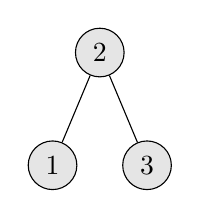
\begin{tikzpicture}
[mynode/.style={draw,circle,minimum size=5mm, fill=gray!20!}]
\node(){};
\node[mynode](1) {2};
\node[mynode](2) [below = 8mm of 1, xshift=-6mm] {1};
\node[mynode](3) [below = 8mm of 1, xshift=6mm] {3};
\draw (1) -- (2);
\draw (1) -- (3);
\end{tikzpicture}
\end{figure}
$p = 1$
\\
\textbf{Output}: 2
\\
\textbf{Explanation}: 
\\
1's in-order successor node is 2. Note that both $p$ and the return value is of \texttt{TreeNode} type.
\end{flushleft}

\paragraph{Example 2:}
\begin{flushleft}
\textbf{Input}:
\begin{figure}[H]
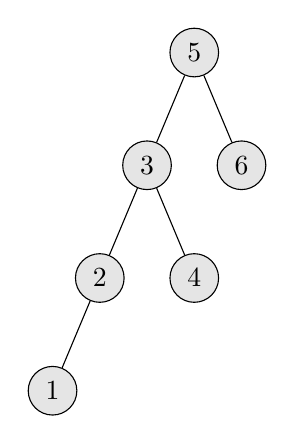
\begin{tikzpicture}
[mynode/.style={draw,circle,minimum size=5mm, fill=gray!20!}]
\node(){};
\node[mynode](1) {5};
\node[mynode](2) [below = 8mm of 1, xshift=-6mm] {3};
\node[mynode](3) [below = 8mm of 1, xshift=6mm] {6};
\node[mynode](4) [below = 8mm of 2, xshift=-6mm] {2};
\node[mynode](5) [below = 8mm of 2, xshift=6mm] {4};
\node[mynode](6) [below = 8mm of 4, xshift=-6mm] {1};
\draw (1) -- (2);
\draw (1) -- (3);
\draw (2) -- (4);
\draw (2) -- (5);
\draw (4) -- (6);
\end{tikzpicture}
\end{figure}
$p = 6$
\\
\textbf{Output}: \texttt{null}
\\
\textbf{Explanation}: 
\\
There is no in-order successor of the current node, so the answer is \texttt{null}.
\end{flushleft}
 

\paragraph{Note:}
\begin{itemize}
    \item If the given node has no in-order successor in the tree, return \texttt{null}.
    \item It's guaranteed that the values of the tree are unique.
\end{itemize}
\subsection{Iterative}
maintain一个 flag $b$,初始化为\texttt{false}。然后进行中序遍历,
\begin{itemize}
    \item 对于遍历到的节点,首先看检查$b$是否为\fcc{true}。如果是,则说明之前遍历到了$p$,那么当前节点就是$p$的succesor,
    \item 如果$b$仍为\fcc{false},则检查遍历到的节点和$p$是否相同,如果相同,则将$b$设为\fcc{true}
\end{itemize}
\setcounter{lstlisting}{0}
\begin{lstlisting}[style=customc, caption={Iterative In-order Traverse}]
TreeNode* inorderSuccessor( TreeNode* root, TreeNode* p )
{
    auto x = root;
    stack<TreeNode*> stk;

    bool bFound = false;

    //in-order traverse
    while( x || !stk.empty() )
    {
        while( x )
        {
            stk.push( x );
            x = x->left;
        }

        x = stk.top();
        stk.pop();

        if( bFound )
        {
            return x;
        }

        if( x == p )
        {
            bFound = true;
        }

        x = x->right;
    }

    return nullptr;
}
\end{lstlisting}
\subsection{Recursive In-Order Traverse}
采用递归方式的中序遍历需要两个全局变量$x$和$y$,分别用来记录父节点和后继节点。
\begin{itemize}
    \item 开始时,初始化为\texttt{null}
    \item 在递归时,对于当前节点$t$,首先检查$x$和$p$是否相同,如果相同,则将$y$赋为$t$,然后$x$ update为$t$,因此在递归过程中,$x$始终是当前访问的节点。
    \item 最后返回$y$即可。
    \item 另外,当检查到$x$和$p$相同,将$y$设为$t$后,不能立即返回,因为如果这时候返回,递归还要回到上一层,$t$又会被访问一次,而$y$就会被设为$t$的parent节点了。所以,还需要继续递归过程。
\end{itemize}
\begin{lstlisting}[style=customc, caption={Recursive In-order Traverse}]
class Solution
{
public:
    TreeNode* inorderSuccessor( TreeNode* root, TreeNode* p )
    {
        inorder( root, p );

        return y;
    }

    void inorder( TreeNode* t, TreeNode* p )
    {
        if( !t )
        {
            return;
        }

        inorder( t->left, p );

        if( x == p )
        {
            //cannot return from here
            //otherwise it will go back
            //to last step and t will be
            //visited again
            y = t;
        }

        x = t;

        inorder( t->right, p );


    }

    TreeNode* x = nullptr;
    TreeNode* y = nullptr;
};
\end{lstlisting}
\subsection{BST Property --- Iterative}
\begin{itemize}
    \item 比较当前节点$t$的value和$p$节点值的大小,如果$t$的value大,说明$p$肯定在$t$的左子树中,反之$p$在$t$的右子树中。
    \item 在整个比较跳转的过程中,在$t$的value比$p$的值大的时候,keep recording $t$。最后当最后$t$变为null退出循环的时候,最后记录的$t$就是$p$的successor。这是因为$p$的在中序遍历的successor的值肯定是比$p$大的。而上述比较跳转过程,则逐步接近到其successor。
\end{itemize}
\begin{lstlisting}[style=customc, caption={BST Property --- Iterative}]
TreeNode* inorderSuccessor( TreeNode* root, TreeNode* p )
{
    auto t = root;
    auto ans = root;

    while( t )
    {
        if( t->val <= p->val )
        {
            t = t->right;
        }
        else
        {
            //always record t when t->val > p->val
            ans = t;
            t = t->left;
        }
    }

    return ans;
}
\end{lstlisting}
\subsection{BST Property --- Recursive}
递归的方法类似,
\begin{itemize}
    \item 当根节点值小于等于$p$节点值,说明$p$的后继节点一定在右子树中,所以对right node递归,
    \item 如果根节点值大于$p$节点值,那么有可能根节点就是$p$的后继节点,或者左子树中的某个节点是$p$的后继节点,所以先对left node递归,如果返回\texttt{null},说明根节点是后继节点,如果不是\texttt{null},即为$p$的successor
\end{itemize}
\begin{lstlisting}[style=customc, caption={BST Property --- Recursive}]
TreeNode* inorderSuccessor( TreeNode* root, TreeNode* p )
{
    if( !root )
    {
        return nullptr;
    }

    if( root->val <= p->val )
    {
        //search in right subtree
        return inorderSuccessor( root->right, p );
    }
    else
    {
        //search in left subtree
        auto next = inorderSuccessor( root->left, p );
        if( !next )
        {
            //The successor must be the root
            return root;
        }

        return next;
    }
}
\end{lstlisting}

\paragraph{Related Problems}
\begin{itemize}
\item \textbf{94. Binary Tree Inorder Traversal}
\item \textbf{173. Binary Search Tree Iterator}
\item \textbf{510. Inorder Successor in BST II}
\end{itemize} %$
\section{285 --- Walls and Gates}
You are given a $m \times n$ 2D grid initialized with these three possible values.
\begin{itemize}
\item $-1$  ---  A wall or an obstacle.
\item $0$ --- A gate.
\item $+\infty$ --- Infinity means an empty room. We use the value $2^{31} - 1 = 2147483647$ to represent $+\infty$ as you may assume that the distance to a gate is less than 2147483647.
\end{itemize}
Fill each empty room with the distance to its nearest gate. If it is impossible to reach a gate, it should be filled with $+\infty$.
\par
For example, given the 2D grid:
\begin{table}[H]
\begin{tabular}{cccc}
$+\infty$ & -1 & 0 & $+\infty$\\
$+\infty$ & $+\infty$ & $+\infty$ & $-1$\\
$+\infty$ &  $-1$ & $+\infty$ & $-1$\\
0 & $-1$ & $+\infty$ & $+\infty$
\end{tabular}
\end{table}

After running your function, the 2D grid should be:

\begin{table}[H]
\begin{tabular}{cccc}
  3 & $-1$ &  0 &  1\\
  2 &  2 &  1 & $-1$\\
  1 & $-1$ &  2 & $-1$\\
  0 & $-1$ &  3 &  4
\end{tabular}
\end{table}
\subsection{Depth First Search}
类似于求Distance Map的问题,
\begin{itemize}
\item 首先遍历整个grid,每次遇到0,以其周围四个相邻点为起点,开始DFS遍历,并带入深度值1
\item 由于题目中的墙是$-1$,而门是$0$,因此可以直接比较当前深度值和当前位置上的值。
\item 如果遇到的值大于当前深度值,我们将位置值赋为当前深度值,并对当前点的四个相邻点开始DFS遍历,注意此时深度值需要加1
\item 这样遍历完成后,所有的位置就被正确地更新
\end{itemize}
\setcounter{lstlisting}{0}
\begin{lstlisting}[style=customc, caption={DFS}]
void wallsAndGates( vector<vector<int>>& rooms )
{
    int m = static_cast<int>( rooms.size() );
    int n = static_cast<int>( rooms[0].size() );

    for( int i = 0; i < m; ++i )
    {
        for( int j = 0; j < n; ++j )
        {
            if( rooms[i][j] == 0 )
            {
                //dist = 0
                dfs( rooms, i, j, 0 );
            }
        }
    }
}

void dfs( vector<vector<int>>& rooms, int i, int j, int dist )
{

    int m = static_cast<int>( rooms.size() );
    int n = static_cast<int>( rooms[0].size() );

    if( i < 0 || i >= m || j < 0 || j >= n || rooms[i][j] < dist )
    {
        return;
    }

    rooms[i][j] = dist;
    //recursive on four directions
    dfs( rooms, i + 1, j, dist + 1 );
    dfs( rooms, i - 1, j, dist + 1 );
    dfs( rooms, i, j + 1, dist + 1 );
    dfs( rooms, i, j - 1, dist + 1 );
}
\end{lstlisting}
\subsection{Breadth First Search}
BFS方法需要借助queue,
\begin{itemize}
\item 首先把门的位置坐标都放入queue中,
\item 对于门位置的四个相邻点,首先判断其是否在grid范围内,并且距离值是否大于上一位置的距离值加1。
\item 如果满足这些条件,将当前位置的距离值设为赋为上一位置的距离值加1,并将该位置坐标放入queue中。
\item 当queue中的元素遍历完了,所有位置的值就被正确地更新了
\end{itemize}
\begin{lstlisting}[style=customc, caption={BFS}]
void wallsAndGates( vector<vector<int>>& rooms )
{
    queue<pair<int, int>> q;

    //The four direction offsets
    vector<vector<int>> dirs{{0, -1}, {-1, 0}, {0, 1}, {1, 0}};

    int m = static_cast<int>( rooms.size() );
    int n = static_cast<int>( rooms[0].size() );

    for( int i = 0; i < m; ++i )
    {
        for( int j = 0; j < n; ++j )
        {
            if( rooms[i][j] == 0 )
            {
                //add gate's coordinate
                //into the queue
                q.emplace( i, j );
            }
        }
    }

    //BFS
    while( !q.empty() )
    {
        int i = q.front().first;
        int j = q.front().second;
        q.pop();

        for( const auto& d : dirs )
        {
            int x = i + d[0];
            int y = j + d[1];
            if( x < 0 || x >= m || y < 0 || y >= n || rooms[x][y] < rooms[i][j] + 1 )
            {
                continue;
            }

            //only update distance for (x,y) when
            //its value is no less than
            //distance of (i,j) plus 1
            rooms[x][y] = rooms[i][j] + 1;

            q.emplace( x, y );
        }
    }
}
\end{lstlisting}

 %$
\section{287 --- Find the Duplicate Number}
Given an array $A$ containing $n + 1$ integers where each integer is between 1 and $n$ (inclusive), prove that at least one duplicate number must exist. Assume that there is only one duplicate number, find the duplicate one.

\paragraph{Example 1:}
\begin{flushleft}
\textbf{Input}: $[1,3,4,2,2]$
\\
\textbf{Output}: 2
\end{flushleft}

\paragraph{Example 2:}
\begin{flushleft}
\textbf{Input}: $[3,1,3,4,2]$
\\
\textbf{Output}: 3
\end{flushleft}

\paragraph{Note:}
\begin{itemize}
\item You must not modify the array (assume the array is read only).
\item You must use only constant, $O(1)$ extra space.
\item Your runtime complexity should be less than $O(n^2)$.
\item There is only one duplicate number in the array, but it could be repeated more than once.
\end{itemize}
\subsection{Detect Cycle And Find The Cycle Start}
\begin{itemize}
\item 与检测链表是否有cycle并找到cycle的起始点类似。
\item 由于存在重复元素,并且$A$中每个值的大小都是1到$n$,而长度又是$n+1$,因此如果将$A[i]$看作index,那么根据$A[i]$的值访问下个元素$A[A[i]]$到最后就会形成cycle。
\item 另外由于0不属于1到$n$,因此$A[0]$肯定不在cycle内,这就相当于有cycle的链表里,链表的头指针不在cycle中。
\item 借用链表中的快慢指针,这里用两个index$x$和$y$分别代表快慢两个index,其中$x\gets A[A[x]]$ 而$y\gets A[y]$。如果遇到相等,就终止循环,
\item 然后$x$和$y$分别从0和刚才循环中断的地方开始按照$i\gets A[i]$的方式前进,直到相等,这个相等的位置处即为重复的number。
\end{itemize}
\setcounter{algorithm}{0}
\begin{algorithm}[H]
\caption{Detect Cycle And Find Cycle Start}
\begin{algorithmic}[1]
\Procedure{FindDuplicate}{$A$}
\State $\ast$ 初始化两个index $x$和$y$为0
\State $\ast$ 检测Cycle,找到快慢两个index的相遇点
\Repeat
\State $x\gets A[A[x]]$
\State $y\gets A[y]$
\Until{$x=y$}
\State $\ast$ 寻找Cycle的起始点
\State $z:=0$ \Comment 找起始点也需要两个index,其中一个是0,另外一个就是刚才找到的相遇点
\Repeat
\State $x\gets A[x]$
\State $z\gets A[z]$
\Until{$x=z$}
\State \Return $x$
\EndProcedure
\end{algorithmic}
\end{algorithm}
\setcounter{lstlisting}{0}
\begin{lstlisting}[style=customc, caption={Detect Cycle And Find Cycle Start}]
int findDuplicate( vector<int>& nums )
{
    //x is the fast index
    //y is the slow index
    int x = 0;
    int y = 0;

    //detect cycle and
    //find the meet point of x and y
    do
    {
        x = nums[nums[x]];
        y = nums[y];
    }
    while( x != y );

    //find the start of the cycle
    //one index will start from 0
    //since nums[0] is not inside cycle
    int z = 0;

    while( x != z )
    {
        x = nums[x];
        z = nums[z];
    }

    return x;
}
\end{lstlisting}
\subsection{Binary Search}
\paragraph{Why Binary Search Can Work}
\begin{enumerate}
\item 由于所有数字的范围都是$1$到$n$,那么如果$A$中没有重复数字,那么对于一个数$x$,在$A$小于或者等于$x$的数字个数就为$x$个。
\item 但由于$A$中有重复的数字,假设这个数字是$m$,那么$A$中小于或者等于这个重复数字$m$的至少有$m+1$个。由于$A$的长度为$n+1$,因此对$A$中其他数,小于或者等于这个数的个数都不会大于这个数本身。
\item 因此binary search是要在$1$到$n$这$n$个数中找到第一个数$\alpha$使得在$A$中小于等于$\alpha$的数的个数$z$要大于$\alpha$。典型的\textbf{rightmost} binary search。
\item 注意binary search不是作用于数组$A$。
\end{enumerate}
\paragraph{Algorithm Steps}
\begin{itemize}
\item 初始化左右两端的index $l$和$r$分别为1和$n$。
\item 得到当前的middle value $x=(l+r)/2$,遍历$A$,得到小于等于$x$的数的count $z$,
\begin{enumerate}
\item 如果$z\leq x$,$l\gets x+1$
\item 如果$z > x$,$r\gets x$
\item 循环结束后 $l$就是那个duplicate number。
\end{enumerate}
\end{itemize}
\begin{algorithm}[H]
\caption{Binary Search}
\begin{algorithmic}[1]
\Procedure{FindDuplicate}{$A,L$}
\State $l:=1$, $r:=L-1$ \Comment Binary Search on $[1,n]$ not on $A$ and $L=n+1$
\State $\ast$ Rightmost Binary Search
\While{$l < r$}
\State $x:=(l+r)/2$ \Comment Mid-point
\State $z:=0$
\For{Each number $t$ in $A$}
\If{$t \leq x$}
\State $z\gets z+1$
\EndIf
\EndFor
\If{$z\leq x$}
\State $l\gets x+1$
\Else
\State $r\gets x$
\EndIf
\EndWhile
\State \Return $l$
\EndProcedure
\end{algorithmic}
\end{algorithm}
\begin{lstlisting}[style=customc, caption={Binary Search}]
int findDuplicate( vector<int>& nums )
{
    int l = 1;
    //r=n
    int r = static_cast<int>( nums.size() ) - 1;

    //binary search on $[1...n]$
    //not on nums
    while( l < r )
    {
        int x = ( l + r ) / 2;

        int count = 0;
        for( int n : nums )
        {
            if( n <= x )
            {
                ++count;
            }
        }

        if( count <= x )
        {
            l = x + 1;
        }
        else
        {
            r = x;
        }
    }

    return l;
}
\end{lstlisting}
\subsection{Bit Manipulation}
\begin{itemize}
\item 在总共32个bit位上,分别统计出1到$n$上在每个比特位上的1的个数,记为$x$
\item 同样的在总共32个bit位上,分别统计出$A$中所有数字在每个比特位上的1的个数,记为$y$。
\item 如果在某个bit位上,$y>x$,表明该位上肯定有重复数字的贡献,因此将结果中的对应的bit位也设为1。
\item 这样32个bit位上设置好相应的bit 1后,就能得到那个重复数字。
\end{itemize}
\setcounter{lstlisting}{0}
\begin{lstlisting}[style=customc, caption={Bit Manipulation}]
int findDuplicate( vector<int>& nums )
{
    int mask = 1;

    int L = static_cast<int>( nums.size() );

    int ans = 0;

    for( int i = 0; i < 32; ++i )
    {
        //in fact, x counts for [0...n]
        //but 0 has no any effect
        mask = 1 << i;

        int x = 0;
        int y = 0;

        for( int i = 0; i < L; ++i )
        {
            if( i & mask )
            {
                ++x;
            }

            if( nums[i] & mask )
            {
                ++y;
            }
        }

        if( y > x )
        {
            ans |= mask;
        }
    }

    return ans;
}
\end{lstlisting}
\section{288 --- Unique Word Abbreviation}
An abbreviation of a word follows the form <first letter><number><last letter>. Below are some examples of word abbreviations:
\begin{enumerate}
\item \texttt{it} --- \texttt{it} (no abbreviation)
\item \texttt{dog} --- \texttt{d1g} (only 1 letter between \textbf{d} and \textbf{g})
\item \texttt{internationalization} --- \texttt{i18n} (There are 18 letters between the first letter \textbf{i} and the last one \textbf{n})
\item  \texttt{localization}  --- \texttt{l10n}
\end{enumerate}
Assume you have a dictionary $A$ and given a word $W$, find whether its abbreviation is unique in the dictionary. A word's abbreviation is \textbf{unique} \textbf{if no other word} from the dictionary has the same abbreviation.

\paragraph{Example: }

Given $A$ = [ \texttt{deer}, \texttt{door}, \texttt{cake}, \texttt{card} ]

\begin{lstlisting}[style=customc]
isUnique("dear") // false
isUnique("cart") // true
isUnique("cane") // false
isUnique("make") // true
\end{lstlisting}
\subsection{Hash Map}
注意题目中的\textbf{if no other word}。例如
\begin{itemize}
\item $A$ = [\texttt{dear}],
\begin{lstlisting}[style=customc]
isUnique("door") // false
\end{lstlisting}
\item $A$ = [\texttt{door}, \texttt{door}]
\begin{lstlisting}[style=customc]
isUnique("door") // true
\end{lstlisting}
\item $A$ = [\texttt{dear}, \texttt{door}]
\begin{lstlisting}[style=customc]
isUnique("door") // false
\end{lstlisting}
\end{itemize}
结合题目中的例子,unique的要求是
\begin{itemize}
\item 如果$A$中所有单词的缩写形式都没有和$W$相同的,是unqiue。
\item 如果有相同的,那么如果这个缩写形式还有除了$W$的其他单词,就不是unique,反之则仍然是unique。
\end{itemize}
因此用一个hash map建立缩写形式和其对应的单词的映射,把所有缩写形式的相同单词放到一个hash set中。在hash map中找不到缩写形式,返回\texttt{true}。如果找到了,而且对应的hash set只有一个单词,且这个单词就是$W$。那么也返回\texttt{true}。
\setcounter{lstlisting}{0}
\begin{lstlisting}[style=customc, caption={Hash Map}]
class ValidWordAbbr
{
public:
    ValidWordAbbr( vector<string> &dictionary )
    {
        for( auto a : dictionary )
        {
            string k = a[0] + to_string( a.size() - 2 ) + a.back();
            auto iter = m.find( k );
            if( iter == m.end() )
            {
                m.emplace( k, initializer_list<string> {a} );
            }
            else
            {
                iter->second.emplace( a );
            }
        }
    }
    bool isUnique( string word )
    {
        string k = word[0] + to_string( word.size() - 2 ) + word.back();
        auto iter = m.find( k );
        if( iter == m.end() )
        {
            return false;
        }
        //iter->second.size()==1
        //and iter->second only contains word
        return iter->second.count( word ) == iter->second.size();
    }
private:
    unordered_map<string, set<string>> m;
};
\end{lstlisting}
\subsection{Memory Efficient}
为了减少内存使用,可以把上述hash map的hash set换成string。当处理字典中的单词时,如果在hash map中找不到当前单词的缩写形式,将该缩写形式和当前单词建立映射,如果该缩写形式已经在hash map中,看对应的单词是不是当前单词,如果不是,就将这个缩写形式对应的值改为空字符串,这样只要字典中一个缩写形式对应一个以上的单词,最终的结果这个缩写形式对应的单词就是空字符串,如果$W$的缩写形式也是能够在hash map中找到,则直接比较$W$和这个缩写形式所对应的字符串,看是否相等。
\begin{lstlisting}[style=customc, caption={Memory Efficient}]
class ValidWordAbbr
{
public:
    ValidWordAbbr( vector<string> &dictionary )
    {
        for( auto a : dictionary )
        {
            string k = a[0] + to_string( a.size() - 2 ) + a.back();
            auto iter = m.find( k );
            if( iter == m.end() )
            {
                m.emplace( k, a );
            }
            else
            {
                //this abbr has already
                //been found in another different word
                if( iter->second != a )
                {
                    iter->second.clear();
                }
            }
        }
    }

    bool isUnique( string word )
    {
        string k = word[0] + to_string( word.size() - 2 ) + word.back();
        auto iter = m.find( k );
        if( iter == m.end() )
        {
            return true;
        }

        return iter->second == word;
    }
private:
    unordered_map<string, string> m;
};
\end{lstlisting}

\paragraph{Related Problems}
\begin{itemize}
\item \textbf{170. Two Sum III - Data structure design}
\item \textbf{320. Generalized Abbreviation}
\end{itemize}
\section{289 --- Game of Life}
According to the \textit{Wikipedia}'s article: 
\begin{quotation}
The Game of Life, also known simply as Life, is a cellular automaton devised by the British mathematician John Horton Conway in 1970.
\end{quotation}

Given a board $B$ with $m\times n$ cells, each cell has an initial state live (1) or dead (0). Each cell interacts with its eight neighbors (horizontal, vertical, diagonal) using the following four rules (taken from the above \textbf{Wikipedia} article):

\begin{enumerate}
\item Any live cell with fewer than two live neighbors dies, as if caused by under-population.
\item Any live cell with two or three live neighbors lives on to the next generation.
\item Any live cell with more than three live neighbors dies, as if by over-population..
\item Any dead cell with exactly three live neighbors becomes a live cell, as if by reproduction.
\end{enumerate}

Write a function to compute the next state (after one update) of the board given its current state. The next state is created by applying the above rules simultaneously to every cell in the current state, where births and deaths occur simultaneously.

\paragraph{Example:}

\begin{flushleft}
\textbf{Input}: 
\begin{table}[H]
\begin{tabular}{lll}
0 & 1 & 0\\
0 & 0 & 1\\
1 & 1 & 1\\
0 & 0 & 0
\end{tabular}
\end{table}

\textbf{Output}: 
\begin{table}[H]
\begin{tabular}{lll}
0 & 0 & 0\\
1 & 0 & 1\\
0 & 1 & 1\\
0 & 1 & 0
\end{tabular}
\end{table}
\end{flushleft}

\paragraph{Follow up:}

\begin{itemize}
\item Could you solve it in-place? Remember that the board needs to be updated at the same time: You cannot update some cells first and then use their updated values to update other cells.
\item In this question, we represent the board using a 2D array. In principle, the board is infinite, which would cause problems when the active area encroaches the border of the array. How would you address these problems?
\end{itemize}
\subsection{In-Place By Bit Manipulation}
\begin{itemize}
\item Each cell只有1或者0这两种状态
\item 为了能够同时保存现有状态和下一步状态,用两个bit位分别代表现有状态和下一步状态,这样就有四种情况
\begin{enumerate}
\item 00 --- 现在是dead,下一步也是dead
\item 01 --- 现在是live,下一步是dead
\item 10 --- 现在是dead,下一步是live
\item 11 --- 现在是live,下一步是live
\end{enumerate}
这样要获取当前状态每个cell中的值只要与1进行相与即可,要获得下一步状态就将cell中的值右移一位。
\item 最开始的时候每个cell的值为$00$或者$01$
\item 因此需要遍历两次$B$,第一次获取下一步状态,第二次则是把上一次状态从每个cell的value中去除。
\end{itemize}
\setcounter{lstlisting}{0}
\begin{lstlisting}[style=customc, caption={In-Place}]
class Solution
{
public:
    void gameOfLife( vector<vector<int>>& board )
    {
        m = static_cast<int>( board.size() );
        n = static_cast<int>( board[0].size() );

        //get next state for each cell
        //current and next state will be
        //in each cell's value
        for( int r = 0; r < m; ++r )
        {
            for( int c = 0; c < n; ++c )
            {
                next( r, c, board );
            }
        }

        //remove last state
        //by right shift one place
        for( int r = 0; r < m; ++r )
        {
            for( int c = 0; c < n; ++c )
            {
                board[r][c] >>= 1;
            }
        }

    }
    //get next state
    void next( int r, int c, vector<vector<int>>& B )
    {
        int state = 0;

        state += live( r - 1, c - 1, B );
        state += live( r - 1, c, B );
        state += live( r - 1, c + 1, B );

        state += live( r, c - 1, B );
        state += live( r, c + 1, B );

        state += live( r + 1, c - 1, B );
        state += live( r + 1, c, B );
        state += live( r + 1, c + 1, B );


        //get current state
        int x = B[r][c] & 1;

        if( x == 1 )
        {
            //cell is live
            if( ( state < 2 ) || ( state > 3 ) )
            {
                //live->dead
                //value for cell: 0x01=1
                B[r][c] = 1;
            }
            else
            {
                //live->live
                //value for cell: 0x11=3
                B[r][c] = 3;
            }
        }
        else
        {
            //current state is dead
            if( state == 3 )
            {
                //dead->live
                //value for cell: 0x10=2
                B[r][c] = 2;
            }
        }

    }

    int live( int r, int c, vector<vector<int>>& B )
    {
        if( ( r >= 0 ) && ( r < m ) && ( c >= 0 ) && ( c < n ) )
        {
            //get current state by and 1
            return B[r][c] & 1;
        }

        return 0;
    }

    int m;
    int n;
};
\end{lstlisting}

\paragraph{Related Problems}
\begin{itemize}
\item \textbf{73. Set Matrix Zeroes}
\end{itemize}
\section{290 --- Word Pattern}
Given a pattern $P$ and a string $S$, find if $S$ follows the same pattern.
\par
Here follow means a full match, such that there is a bijection between a letter in $P$ and a non-empty word in $S$.

\paragraph{Example 1:}
\begin{flushleft}
\textbf{Input}: $P$ = \texttt{abba}, $S$ = \texttt{dog cat cat dog}
\\
\textbf{Output}: \texttt{true}
\end{flushleft}

\paragraph{Example 2:}
\begin{flushleft}
Input: $P$ = \texttt{abba}, $S$ = \texttt{dog cat cat fish}
\\
Output: \texttt{false}
\end{flushleft}

\paragraph{Example 3:}
\begin{flushleft}
\textbf{Input}: $P$ = \texttt{aaaa}, $S$ = \texttt{dog cat cat dog}
\\
\textbf{Output}: \texttt{false}
\end{flushleft}

\paragraph{Example 4:}
\begin{flushleft}
\textbf{Input}: $P$ = \texttt{abba}, $S$ = \texttt{dog dog dog dog}
\\
\textbf{Output}: \texttt{false}
\end{flushleft}

\paragraph{Notes:}
\begin{itemize}
\item You may assume $P$ contains only lowercase letters, and $S$ contains lowercase letters separated by a single space.
\end{itemize}
\subsection{Hash Map}
这道题并不难。但是如果自己手动写分割字符串,有几点需要注意
\begin{itemize}
\item 需要考虑$P$和$S$中$P$的长度和$S$中单词个数不相等的情况。
\item 如果只是建立$P$中的letter和$S$中的word的map并不够,比如$P$=\texttt{abba},$S$=\texttt{cat cat cat cat}",这时候letter $a$和$b$都map到了同一个word即\texttt{cat}上,但是不会产生错误
\item 因此还需要一个hash set用来记录已经出现的word,当发现一个letter没有对应的word时,先检查这个word有没有在hash set中,如果有,表示之前有letter已经和这个word对应了。
\end{itemize}
\setcounter{lstlisting}{0}
\begin{lstlisting}[style=customc, caption={Hash Map}]
bool wordPattern( string pattern, string str )
{
    //letter to word map
    vector<string> m( 26 );

    //word sets
    unordered_set<string> ss;

    size_t start = 0;
    size_t count = 0;

    for( auto c : pattern )
    {
        auto p = str.find( ' ', start );

        auto word = str.substr( start, p - start );

        start = p + 1;

        if( m[c - 'a'].empty() )
        {
            if( ss.find( word ) != ss.end() )
            {
                //This word has been already
                //mapped by another letter
                return false;
            }

            m[c - 'a'] = word;
            ss.emplace( word );
        }
        else
        {
            if( m[c - 'a'] != word )
            {
                //The word is different from the word mapped
                //from the same letter
                return false;
            }
        }

        //increments the valid match count
        ++count;

        if( p == string::npos )
        {
            start = str.size();
            break;
        }
    }

    if( start < str.size() )
    {
        //str is longer
        return false;
    }

    //The valid match count must equal to
    //the number letters of pattern
    return count == pattern.size();
}
\end{lstlisting}


\section{291 --- Word Pattern II}
Given a pattern $P$ and a string $S$, find if $S$ follows the same pattern.
\par
Here follow means a full match, such that there is a bijection between a letter in pattern $P$ and a non-empty substring in $S$.

\paragraph{Example 1:}
\begin{flushleft}
\textbf{Input}: $P$ = \texttt{abba}, $S$ = \texttt{redblueredblue}
\\
\textbf{Output}: \texttt{true}
\end{flushleft}

\paragraph{Example 2:}
\begin{flushleft}
\textbf{Input}: $P$ = \texttt{aaaa}, $S$ = \texttt{asdasdasdasd}
\\
\textbf{Output}: \texttt{true}
\end{flushleft}

\paragraph{Example 3:}
\begin{flushleft}
\textbf{Input}: $P$ = \texttt{aabb}, $S$ = \texttt{xyzabcxzyabc}
\\
\textbf{Output}: \texttt{false}
\end{flushleft}

\paragraph{Notes:}
\begin{itemize}
\item You may assume both $P$ and $S$ contains only lowercase letters.
\end{itemize}
\subsection{Backtracking With Hash Map}
与290 --- Word Pattern类似,需要一个hash map和一个hash set。
\begin{itemize}
\item 由于没有空格分隔,只能从开头一个个测试$P$中的letter和$S$中对应的substr。
\item 用$x$和$y$来记录当前处理的$P$和$S$的起始位置,如果$x$和$y$分别等于$P$和$S$的长度,说明此时匹配成功结束了,返回\texttt{ture}。
\item 如果$x$和$y$只有一个等于其对应的字符串的长度,说明匹配失败了,返回\texttt{false}。
\item 如果都不满足上述条件的话,取出当前的$P[x]$,然后从$S$的$y$位置开始往后遍历,每次取出一个单词,如果$P[x]$已经在hash map中,而且对应的单词和取出的单词也相等,那么继续调用递归函数,这时候$x$和$y$都加1。如果递归结果是\texttt{true},就返回\texttt{true}。
\item 如果$P[x]$不在hash map中,需要检查当前在$S$中以$y$开头的word是否在hash set中存在,如果不存在,则将这个word加入hash
 map和hash set,然后继续递归,如果递归结果是\texttt{true},就返回\texttt{true},但如果返回\texttt{false}了,则要将这个word从hash map和hash set中删除。
\end{itemize}
注意,递归函数中,需要对$S$进行循环测试,而$P$是不需要的,因为我们要对于当前$P[x]$测试从$y$开始的所有$S$的substr。另外,由于题目中说明了$P$和$S$中只有小写字母,因此hash map实际上可以用一个大小为26的字符串数组代替。
\setcounter{algorithm}{0}
\begin{algorithm}[H]
\caption{Backtracking}
\begin{algorithmic}[1]
\Procedure{WordPatternMatch}{$P, S$}
\State $\star$ 初始化一个hash map $M$和一个hash set $T$
\State $\ast$ $P$ and $S$ are all empty --- Matched
\If{$P$ is empty \textbf{and} $S$ is empty}
\State \Return \texttt{true}
\EndIf
\State $\ast$ Only one of $P$ and $S$ is empty --- Not Matched
\If{$P$ is empty \textbf{or} $S$ is empty}
\State \Return \texttt{false}
\EndIf
\State \Call{DFS}{$x=0,y=0,P,S,M,T$} \Comment Start backtracking process
\EndProcedure
\end{algorithmic}
\end{algorithm}
Function \texttt{DFS} 递归检查$P$和$S$是否匹配,其中$x$,$y$分别为当前$P$和$S$的起始位置,初始都为零。$M$和$T$则是上面提到的hash map和hash set。
\begin{algorithm}[H]
\caption{Helper Function}
\begin{algorithmic}[1]
\Procedure{DFS}{$x,y,P,S,M,T$}
\If{$x=L_P$ \textbf{and} $y=L_S$} \Comment $x$和$y$都刚好到达$P$和$S$的末尾,匹配成功
\State \Return \texttt{true}
\EndIf
\If{$x=L_P$ \textbf{or} $y=L_S$} \Comment $x$和$y$中只有一个都刚好到达对应字符串的末尾,匹配失败
\State \Return \texttt{true}
\EndIf
\algstore{291algo}
\end{algorithmic}
\end{algorithm}
\begin{algorithm}[H]
\begin{algorithmic}[1]
\algrestore{291algo}
\For{$i:=y$ \textbf{to} $L_S-1$}
\State $W:=S[y\ldots i]$ \Comment 当前检查的word
\If{$P[x]$ is not in $M$} \label{291if1}
\State $\star$ $W$不能在以前出现过,否则$W$已经和$P$中的另外一个letter建立了对应关系
\If{$W$ is not in $T$}
\State $\star$ 将$W$加入$M$和$T$中
\State $\ast$ 继续到$x+1$和$y+1$继续进行递归
\State $b:=$\Call{DFS}{$x+1,y+1,P,S,M,T}$
\If{$b$ is \texttt{true}}
\State \Return \texttt{true} \Comment $P$ and $S$ is matched
\EndIf
\EndIf
\Else
\If{$M[i] = W$} \Comment letter $P[x]$ 对应的word和当前的word相等
\State $\ast$ 继续到$x+1$和$y+1$继续进行递归
\State $b:=$\Call{DFS}{$x+1,y+1,P,S,M,T}$
\If{$b$ is \texttt{true}}
\State \Return \texttt{true} \Comment $P$ and $S$ is matched
\EndIf
\EndIf
\EndIf \Comment End[\ref{291if1}]
\EndFor
\State \Return \texttt{false}
\EndProcedure
\end{algorithmic}
\end{algorithm}
\setcounter{lstlisting}{0}
\begin{lstlisting}[style=customc, caption={Backtracking}]
bool wordPatternMatch( string pattern, string str )
{
    if( pattern.empty() && str.empty() )
    {
        return true;
    }

    if( pattern.empty() || str.empty() )
    {
        return false;
    }

    vector<string> m( 26 );
    unordered_set<string> ss;

    return dfs( 0, 0, pattern, str, m, ss );
}

bool dfs( size_t x, size_t y, const string& P, const string& S, vector<string>& m, unordered_set<string>& ss )
{
    if( x == P.size() && y == S.size() )
    {
        return true;
    }

    if( ( x >= P.size() ) || ( y >= S.size() ) )
    {
        return false;
    }

    int ci = P[x] - 'a';

    //loop from y to until end of S
    //to test each word S[y...j]
    for( size_t j = y; j < S.size(); ++j )
    {
        auto word = S.substr( y, j - y + 1 );

        if( m[ci].empty() )
        {
            if( ss.find( word ) == ss.end() )
            {
                //this word has not been appeared before
                ss.emplace( word );
                m[ci] = word;

                //continue DFS from next position
                if( dfs( x + 1, j + 1, P, S, m, ss ) )
                {
                    return true;
                }

                ss.erase( m[ci] );

                m[ci].clear();

            }

        }
        else
        {
            if( m[ci] == word )
            {
                //S[y...i] is equal to the word mapped by the
                //letter P[x], continue DFS from next position
                if( dfs( x + 1, j + 1, P, S, m, ss ) )
                {
                    return true;
                }
            }
        }
    }
    return false;
}
\end{lstlisting} %$
\section{292 --- Nim Game}
You are playing the following \textit{Nim Game} with your friend: There is a heap of stones on the table, each time one of you take turns to remove 1 to 3 stones. The one who removes the last stone will be the winner. You will take the first turn to remove the stones.
\par
Both of you are very clever and have optimal strategies for the game. Write a function to determine whether you can win the game given the number of stones in the heap.

\paragraph{Example:}

\begin{flushleft}
\textbf{Input}: 4
\\
\textbf{Output}: \texttt{false} 
\\
\textbf{Explanation}: 
\\
If there are 4 stones in the heap, then you will never win the game; No matter 1, 2, or 3 stones you remove, the last stone will always be removed by your friend.
\end{flushleft}
\subsection{Mathematical Analysis}
You can always win a Nim game if the number of stones $n$ in the pile is not divisible by 4.

\paragraph{Reasoning}

Let us think of the small cases. It is clear that if there are only 1, 2, or 3 stones in the pile, and it is your turn, you can win the game by taking all of them. 
\par
If there are exactly four stones in the pile, you will lose. Because no matter how many you take, you will leave some stones behind for your opponent to take and win the game.
\par
So in order to win, you have to ensure that you never reach the situation where there are exactly 4 stones on the pile on your turn.
\par
Similarly, if there are 5, 6, or 7 stones you can win by taking just enough to leave 4 stones for your opponent so that they lose. 
\par
But if there are 8 stones on the pile, you will inevitably lose, because regardless whether you pick 1, 2 or 3 stones from the pile, your opponent can pick 3, 2 or 1 stone to ensure that four stones will be left to you on your turn.
\par
It is obvious that the same pattern repeats itself for $n=4,8,12,16,\dots$. Basically all multiples of 4. 
\section{293 --- Flip Game }
You are playing the following Flip Game with your friend: Given a string that contains only these two characters: \fcj{'+'} and \fcj{'-'}, you and your friend take turns to flip two consecutive \fcj{"++"} into \fcj{"--"}. The game ends when a person can no longer make a move and therefore the other person will be the winner.

Write a function to compute all possible states of the string after one valid move.

\begin{flushleft}
Example:

\textbf{Input}: \fcj{s = "++++"}

\textbf{Output}: 

  \fcj{"--++"}
  
  \fcj{"+--+"}
  
  \fcj{"++--"}
\end{flushleft}

If there is no valid move, return an empty list.
\subsection{Analysis}
很简单的题目,从第二个字母开始遍历,每次判断当前字母是否为\fcj{'+'},和之前那个字母是否为\fcj{'+'},如果都是,则将翻转后的字符串存入结果中。
\setcounter{lstlisting}{0}
\begin{lstlisting}[style=customc, caption={Loop}]
vector<string> generatePossibleNextMoves( string s )
{
    vector<string> ans;
    for( int i = 1; i < s.size(); ++i )
    {
        if( s[i] == '+' && s[i - 1] == '+' )
        {
            ans.push_back( s.substr( 0, i - 1 ) + "--" + s.substr( i + 1 ) );
        }
    }
    return ans;
}
\end{lstlisting}

\paragraph{Related Problems}
\begin{itemize}
\item \textbf{294. Flip Game II}
\end{itemize} %$
\section{294 --- Flip Game II}
You are playing the following Flip Game with your friend: Given a string that contains only these two characters: \fcj{'+'} and \fcj{'-'}, you and your friend take turns to flip two consecutive \fcj{"++"} into \fcj{"--"}. The game ends when a person can no longer make a move and therefore the other person will be the winner
.
Write a function to determine if the starting player can guarantee a win.

\paragraph{Example}:

\begin{flushleft}
\textbf{Input}: \fcj{s = "++++"}

\textbf{Output}: \fcj{true} 

\textbf{Explanation}:

The starting player can guarantee a win by flipping the middle \fcj{"++"} to become \fcj{"+--+"}.
\end{flushleft}

\paragraph{Follow up:}
\begin{itemize}
\item Derive your algorithm's runtime complexity.
\end{itemize}
\subsection{Backtracking}
此题同样也是用Backtracking,从第二个字母开始遍历整个字符串,如果当前字母和之前那个字母都是\fcj{"+"},将其变为\fcj{"--"},然后递归检查这个字符串,如果返回\fcj{false},说明当前玩家可以赢,因为那个结果是另一个玩家的结果。
\setcounter{lstlisting}{0}
\begin{lstlisting}[style=customc, caption={Backtracking}]
bool canWin( string s )
{
    return dfs( s );
}
bool dfs( string& s )
{
    for( size_t i = 1; i < s.size(); ++i )
    {
        if( ( s[i] == '+' ) && ( s[i - 1] == '+' ) )
        {
            s[i - 1] = '-';
            s[i] = '-';
            //opponent lost
            //means I win
            bool win = !dfs( s );
            //backtrack
            //we have to backtrack first
            //then check the result
            s[i - 1] = '+';
            s[i] = '+';
            if( win )
            {
                return true;
            }
        }
    }
    return false;
}

\end{lstlisting}


 %$
\section{295 --- Find Median from Data Stream}
Median is the middle value in an ordered integer list. If the size of the list is even, there is no middle value. So the median is the mean of the two middle value.
\par
For example,
\par
$[2,3,4]$, the median is 3
\par
$[2,3]$, the median is $(2 + 3) / 2 = 2.5$
\par
Design a data structure that supports the following two operations:

\begin{lstlisting}[style=customc]
// Add a integer number from the data stream to the data structure.
void addNum(int num);
// Return the median of all elements so far. 
double findMedian(); 
\end{lstlisting}
 

\paragraph{Example:}

\begin{flushleft}
\begin{lstlisting}[style=customc]
addNum(1);
addNum(2);
findMedian(); //1.5
addNum(3); 
findMedian(); // 2
\end{lstlisting}
\end{flushleft}

\paragraph{Follow up:}

\begin{itemize}
\item If all integer numbers from the stream are between 0 and 100, how would you optimize it?
\item If 99\% of all integer numbers from the stream are between 0 and 100, how would you optimize it?
\end{itemize}
\section{296 --- Best Meeting Point}
A group of two or more people wants to meet and minimize the total travel distance. You are given a 2D grid of values 0 or 1, where each 1 marks the home of someone in the group. The distance is calculated using Manhattan Distance, where distance$(p_1, p_2) = \lvert p_2.x - p_1.x\rvert + \lvert p_2.y - p_1.y \rvert$.
\par
For example, given three people living at $(0,0)$, $(0,4)$, and $(2,2)$:
\begin{table}[H]
\begin{tabular}{ccccc}
1 & 0 & 0 & 0 & 1\\
0 & 0 & 0 & 0 & 0\\
0 & 0 & 1 & 0 & 0
\end{tabular}
\end{table}
The point $(0,2)$ is an ideal meeting point, as the total travel distance of $2+2+2=6$ is minimal. So return 6.

\paragraph{Hint:}

\begin{itemize}
\item Try to solve it in one dimension first. How can this solution apply to the two dimension case?
\end{itemize}
\subsection{Sorting}
根据题目中的提示,先从一维的情况分析,假设只有两个点$A$和$B$,那么显然最佳的meeting点$P$肯定是在$A$和$B$之间,而$A$和$B$中间任何一点到$A$和$B$的距离之和就是$A$和$B$的距离。
\begin{figure}[H]
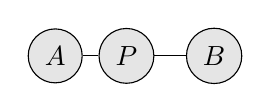
\begin{tikzpicture}
[mynode/.style={draw,circle,minimum size=5mm, fill=gray!20!}]
\node(){};
\node[mynode](1) {$A$};
\node[mynode](2) [right = 2mm of 1] {$P$};
\node[mynode](3) [right = 4mm of 2] {$B$};
\draw (1) -- (2);
\draw (2) -- (3);
\end{tikzpicture}
\end{figure}

如果在$A$,$B$之外再加两个点$C$和$D$:

\begin{figure}[H]
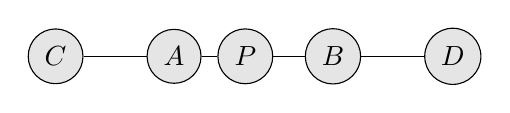
\begin{tikzpicture}
[mynode/.style={draw,circle,minimum size=5mm, fill=gray!20!}]
\node(){};
\node[mynode](1) {$C$};
\node[mynode](2) [right = 8mm of 1] {$A$};
\node[mynode](3) [right = 2mm of 2] {$P$};
\node[mynode](4) [right = 4mm of 3] {$B$};
\node[mynode](5) [right = 8mm of 4] {$D$};
\draw (1) -- (2);
\draw (2) -- (3);
\draw (3) -- (4);
\draw (4) -- (5);
\end{tikzpicture}
\end{figure}
同样,最佳meeting点$P$点的位置还是在$[A, B]$内,这时$P$到$A$,$B$,$C$,$D$和四个点的距离之和即为$A$和$B$之间的距离加上$C$和$D$之间的距离,
\par
\begin{itemize}
    \item 将所有1的点的$x$和$y$的坐标分别放入两个数组中,然后排序这两个数组。
    \item 对每个数组,用最后一个值减去第一个值,就是最外围两个点之间的距离,然后倒数第二个值减去第二个值,以此类推,直到最中间停止。
    \item 累加这些距离值就分别是$x$和$y$方向上的最短距离和。由于题目中要求的是曼哈顿距离,因此只要把$x$和$y$方向的距离分别计算处理,直接相加就是所要求的最短距离和了。
\end{itemize}
\setcounter{lstlisting}{0}
\begin{lstlisting}[style=customc, caption={Sorting}]
int minTotalDistance( vector<vector<int>>& grid )
{
    vector<int> rows;
    vector<int> cols;

    int m = static_cast< int >( grid.size() );
    int n = static_cast< int >( grid[0].size() );

    rows.reserve( m );
    cols.reserve( n );

    for( int i = 0; i < m; ++i )
    {
        for( int j = 0; j < n; ++j )
        {
            if( grid[i][j] == 1 )
            {
                rows.push_back( i );
                cols.push_back( j );
            }
        }
    }

    int distX = minDist( rows );
    int distY = minDist( cols );

    //The distance is manhattan distance
    return distX + distY;
}

int minDist( vector<int>& pts )
{
    sort( pts.begin(), pts.end() );

    int l = 0;
    int r = static_cast< int >( pts.size() ) - 1;

    int dist = 0;

    //Find distance of each end
    while( l < r )
    {
        dist += ( pts[r] - pts[l] );
        ++l;
        --r;
    }

    return dist;
}
\end{lstlisting} %$
\section{297 --- Serialize and Deserialize Binary Tree}
Serialization is the process of converting a data structure or object into a sequence of bits so that it can be stored in a file or memory buffer, or transmitted across a network connection link to be reconstructed later in the same or another computer environment.
\par
Design an algorithm to \textbf{serialize} and \textbf{deserialize} a binary tree. There is no restriction on how your serialization/deserialization algorithm should work. You just need to ensure that a binary tree can be serialized to a string and this string can be deserialized to the original tree structure.

\paragraph{Example: }

\begin{flushleft}
You may serialize the following tree:
\begin{figure}[H]
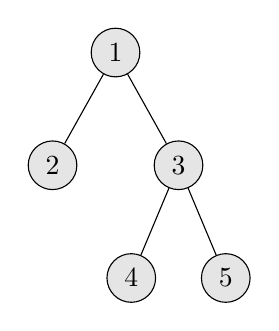
\begin{tikzpicture}
[mynode/.style={draw,circle,minimum size=5mm, fill=gray!20!}]
\node(){};
\node[mynode](a) {1};
\node[mynode](b)[below=8mm of a, xshift=-8mm] {2};
\node[mynode](c)[below=8mm of a, xshift=8mm] {3};
\node[mynode](d)[below=8mm of c, xshift=-6mm] {4};
\node[mynode](e)[below=8mm of c, xshift=6mm] {5};
\draw (a) -- (b);
\draw (a) -- (c);
\draw (c) -- (d);
\draw (c) -- (e);
\end{tikzpicture}
\end{figure}
as \fcj{[1,2,3,null,null,4,5]}
\end{flushleft}

\paragraph{Clarification:}
\begin{flushleft}
The above format is the same as how \textbf{LeetCode} serializes a binary tree. You do not necessarily need to follow this format, so please be creative and come up with different approaches yourself.
\end{flushleft}

\subsection{Preorder}
In serialization, we visit the tree with preorder sequence. Using \fcj{null} to represent the empty node, and separate each node with a comma.

In deserializaton, we splice the given string, and then initiate the node value, and then calls itself to construct its left and right child nodes.



\section{298 --- Binary Tree Longest Consecutive Sequence}
Given a binary tree, find the length of the longest consecutive sequence path.
\par
The path refers to any sequence of nodes from some starting node to any node in the tree along the parent-child connections. The longest consecutive path need to be from parent to child (cannot be the reverse).

\paragraph{Example:}

\begin{flushleft}

\begin{figure}[H]
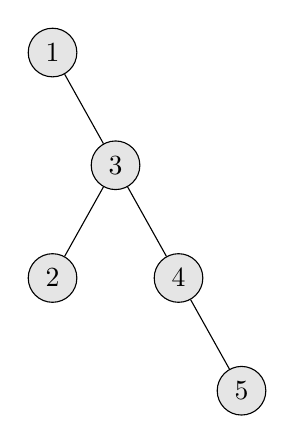
\begin{tikzpicture}
[mynode/.style={draw,circle,minimum size=5mm, fill=gray!20!}]
\node(){};
\node[mynode](a) {1};
\node[mynode](b)[below=8mm of a, xshift=8mm] {3};
\node[mynode](c)[below=8mm of b, xshift=-8mm] {2};
\node[mynode](d)[below=8mm of b, xshift=8mm] {4};
\node[mynode](e)[below=8mm of d, xshift=8mm] {5};
\draw (a) -- (b);
\draw (b) -- (c);
\draw (b) -- (d);
\draw (d) -- (e);
\end{tikzpicture}
\end{figure}

Longest consecutive sequence path is 3--4--5, so return 3.

\begin{figure}[H]
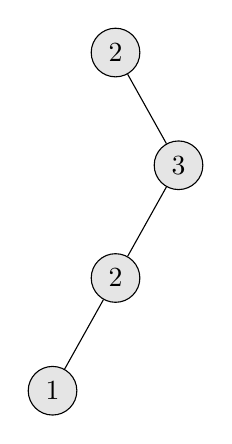
\begin{tikzpicture}
[mynode/.style={draw,circle,minimum size=5mm, fill=gray!20!}]
\node(){};
\node[mynode](a) {2};
\node[mynode](b)[below=8mm of a, xshift=8mm] {3};
\node[mynode](c)[below=8mm of b, xshift=-8mm] {2};
\node[mynode](d)[below=8mm of c, xshift=-8mm] {1};
\draw (a) -- (b);
\draw (b) -- (c);
\draw (c) -- (d);
\end{tikzpicture}
\end{figure}

Longest consecutive sequence path is 2--3,not 3--2--1, so return 2.
\end{flushleft}
\subsection{Depth First Search}
\begin{itemize}
\item 对当前节点$t$的left and right node分别处理,
\item 如果left node存在且值比$t$的值大1,则递归处理left node,同时递归调用函数输入参数中的当前长度加1。否则,还是递归处理left node,但是输入参数中的当前长度重置为1。
\item 对于right node的处理情况和left node相同。
\item 处理完左右节点,需要和当前的结果进行比较,得到最大的那个length。
\end{itemize}
\setcounter{lstlisting}{0}
\begin{lstlisting}[style=customc, caption={DFS}]
int longestConsecutive( TreeNode* root )
{
    if( !root )
    {
        return 0;
    }

    int ans = 0;

    dfs( root, 1, ans );

    return ans;
}

void dfs( TreeNode *t, int len, int &ans )
{
    ans = max( ans, len );

    if( t->left )
    {
        if( t->left->val == t->val + 1 )
        {
			//len<-len+1
            dfs( t->left, len + 1, ans );
        }
        else
        {
			//reset len to 1
            dfs( t->left, 1, ans );
        }
    }

    if( t->right )
    {
        if( t->right->val == t->val + 1 )
        {
            //len<-len+1
            dfs( t->right, len + 1, ans );
        }
        else
        {
            //reset len to 1
            dfs( t->right, 1, ans );
        }
    }
}

\end{lstlisting}
另外一种更简洁的代码如下
\begin{lstlisting}[style=customc, caption={DFS 2}]
int longestConsecutive( TreeNode* root )
{
    return dfs( root, nullptr, 0 );
}

int dfs( TreeNode *t, TreeNode *parent, int len )
{
    if( !t )
    {
        return len;
    }

    if( parent && ( t->val == parent->val + 1 ) )
    {
        ++len;
    }
    else
    {
        len = 1;
    }

    int l_len = dfs( t->left, t, len );
    int r_len = dfs( t->right, t, len );

    return ( max )( len, ( max )( l_len, r_len ) );
}
\end{lstlisting} %$
\section{299 --- Bulls and Cows}
You are playing the following \textbf{Bulls and Cows} game with your friend: You write down a number and ask your friend to guess what the number is. Each time your friend makes a guess, you provide a hint that indicates how many digits in said guess match your secret number exactly in both digit and position (called \textit{bulls}) and how many digits match the secret number but locate in the wrong position (called \textit{cows}). Your friend will use successive guesses and hints to eventually derive the secret number.

Write a function to return a hint according to the secret number and friend's guess, use $A$ to indicate the bulls and $B$ to indicate the cows. 

Please note that both secret number and friend's guess may contain duplicate digits.

\paragraph{Example 1:}

\begin{flushleft}
\textbf{Input}: \fcj{secret = "1807"},\fcj{ guess = "7810"}
\\
\textbf{Output}: \fcj{"1A3B"}
\\
\textbf{Explanation}: 1 bull and 3 cows. The bull is 8, the cows are 0, 1 and 7.
\end{flushleft}

\paragraph{Example 2:}

\begin{flushleft}
\textbf{Input}: \fcj{secret = "1123"}, \fcj{guess = "0111"}
\\
\textbf{Output}: \fcj{"1A1B"}
\\
\textbf{Explanation}: The 1st 1 in friend's guess is a bull, the 2nd or 3rd 1 is a cow.
\end{flushleft}

\paragraph{Note:} 
\begin{itemize}
\item You may assume that the secret number and your friend's guess only contain digits, and their lengths are always equal.
\end{itemize}
\subsection{Tricks}
\begin{itemize}
\item 算法思路: iterate over secret $S$ 和 guess $G$,首先可以很快得到所有bulls的(即数字和出现位置都相等)。对于cows(即数字相同,但是出现位置不同),则maintain一个array用于记录数字在$S$和$G$中的出现次数。技巧在于,对于$G$中的数字的出现次数,用负数来表示。
\item 如果$S$当前位置数字的出现次数小于0,则表示其在$G$中出现过,increments cows,同时increments对应的出现次数,
\item 如果$G$当前位置数字的出现次数大于0,则表示其在$S$中出现过,同样increments cows,但是要decrements对应的出现次数。
\end{itemize}

\setcounter{lstlisting}{0}
\begin{lstlisting}[style=customc, caption={Counts}]
string getHint( string secret, string guess )
{
    vector<int> count( 10, 0 );

    int A = 0;
    int B = 0;

    for( size_t i = 0; i < secret.size(); ++i )
    {
        if( secret[i] == guess[i] )
        {
            ++A;
        }
        else
        {
            if( count[secret[i] - '0'] < 0 )
            {
                //secret[i] appeared in guess
                ++B;
            }

            //increments the count of secret[i]
            ++count[secret[i] - '0'];

            if( count[guess[i] - '0'] > 0 )
            {
                //guess[i] appeared in secret
                ++B;
            }
            //decrements the count of guess[i]
            --count[guess[i] - '0'];
        }
    }

    string ans = to_string( A );
    ans.push_back( 'A' );
    ans += to_string( B );
    ans.push_back( 'B' );

    return ans;
}
\end{lstlisting}
\subsection{Two Pass}
\begin{itemize}
\item 算法本质和上述方法是一样的
\item 这里需要两个array,分别记录$S$和$G$中的数字出现的次数。
\item 同样的 iterate over secret $S$ 和 guess $G$,很快得到所有bulls的(即数字和出现位置都相等)。
\item 否则的话,分别increment $S$和$G$在当前位置的数字的次数。
\item 最后,同时遍历$S$和$G$(因为两个长度都是10),然后取其中的较小值加到$B$中。
\end{itemize}

\begin{lstlisting}[style=customc, caption={Two Pass}]
string getHint( string secret, string guess )
{
    vector<int> s_count( 10, 0 );
    vector<int> g_count( 10, 0 );
    int A = 0;
    int B = 0;
    for( size_t i = 0; i < secret.size(); ++i )
    {
        if( secret[i] == guess[i] )
        {
            ++A;
        }
        else
        {
            ++s_count[secret[i] - '0'];
            ++g_count[guess[i] - '0'];
        }
    }

    for( int i = 0; i < 10; ++i )
    {
        B += ( min )( s_count[i], g_count[i] );
    }

    string ans = to_string( A );
    ans.push_back( 'A' );
    ans += to_string( B );
    ans.push_back( 'B' );

    return ans;
}
\end{lstlisting}
\end{document}









